
\documentclass[12pt]{article}
\usepackage{graphicx,caption} % Required for inserting images
\usepackage{algpseudocode}
\usepackage{amsmath}
\usepackage{amsfonts}
\usepackage{mathtools}

\usepackage{subcaption}  % in preamble

\newcommand{\pr}{\hspace{0.05in}}
\newcommand{\pd}{\partial}
\newcommand{\nrm}{\parallel}
\usepackage{pdfpages}
\usepackage{caption}

\def\qd{\hskip1em\relax}
\def\myQuad{\hskip\fontdimen6\font}

\usepackage{tikz}
\usepackage{minted}


%\usepackage[a5paper]{geometry}

%\title{svdX}

\title{algorithmicx (algpseudocode) example}
%\author{starobin }
%\date{March 2024}

\begin{document}
%\maketitle
%\section*{Introduction}
\paragraph{ A mis-use of Sylvester's equation  \small{ Andrei Starobin, 6-3-2026 } } % 12-02-2025

%Comment re organization: Each problem begins following a near-blank page with problem number on it. Hand written solution section ( image scans ) are 
%followed by numerical checks ( these include state space solution and code and LTSpice results. in some plots abbreviation ss == state space and not steady state ) 

%In previous classes Ive had comments 
%about my handwriting and difficulty of following. Looking for feedback. This is an attempt to get away from Latex-ing everything which is SIGNIFICANTLY more time 
%consuming. 

%\paragraph{Re problems  1 and 2 }
%These were done before the update on HW scope, so are included in this submission. In this submission they show up 
%as P4 and P5 at the beginning 

%\paragraph{ Re calculating to asymptotes for phase } 
%The linear slope construction for 1st order terms is a good one. In most of this submission I use E105 type step asymptotes and then use some 
%side rules for atan on the linear-log phase plot to draw the phase components. Each term is drawn separately ( as dashed lines ) and then graphically these 
%are added approximately. 

%\paragraph{ Submission 2 } 

Consider the following Sylvester's equation mis-use: 

\begin{minted}[fontsize=\footnotesize]{julia}
X  = sylvester( g1 + 1e-3 * eye(8), -g2, 1e-3 * eye(8) )
qq = abs.(inv(X) * g1 * X) .>1e-1

% a check
qq .* g2 - g2
\end{minted}

\paragraph{ }

\begin{align}
g_1 = 
%\begin{matrix}
\left[\begin{array}{rrrrrrrr}
0 &1 &0 &1 &0 &0 &0 &0 \\ 
-1 &0 &1 &-1 &0 &0 &0 &0 \\ 
0 &-1 &0 &-1 &-1 &0 &0 &0 \\ 
-1 &1 &1 &0 &1 &0 &0 &0 \\ 
0 &0 &1 &-1 &0 &0 &0 &0 \\ 
0 &0 &0 &0 &0 &0 &1 &-1 \\ 
0 &0 &0 &0 &0 &-1 &0 &-1 \\ 
0 &0 &0 &0 &0 &1 &1 &0  
%\end{matrix}
\end{array}\right]
\end{align}

\begin{figure}[!htbp]
\begin{center}
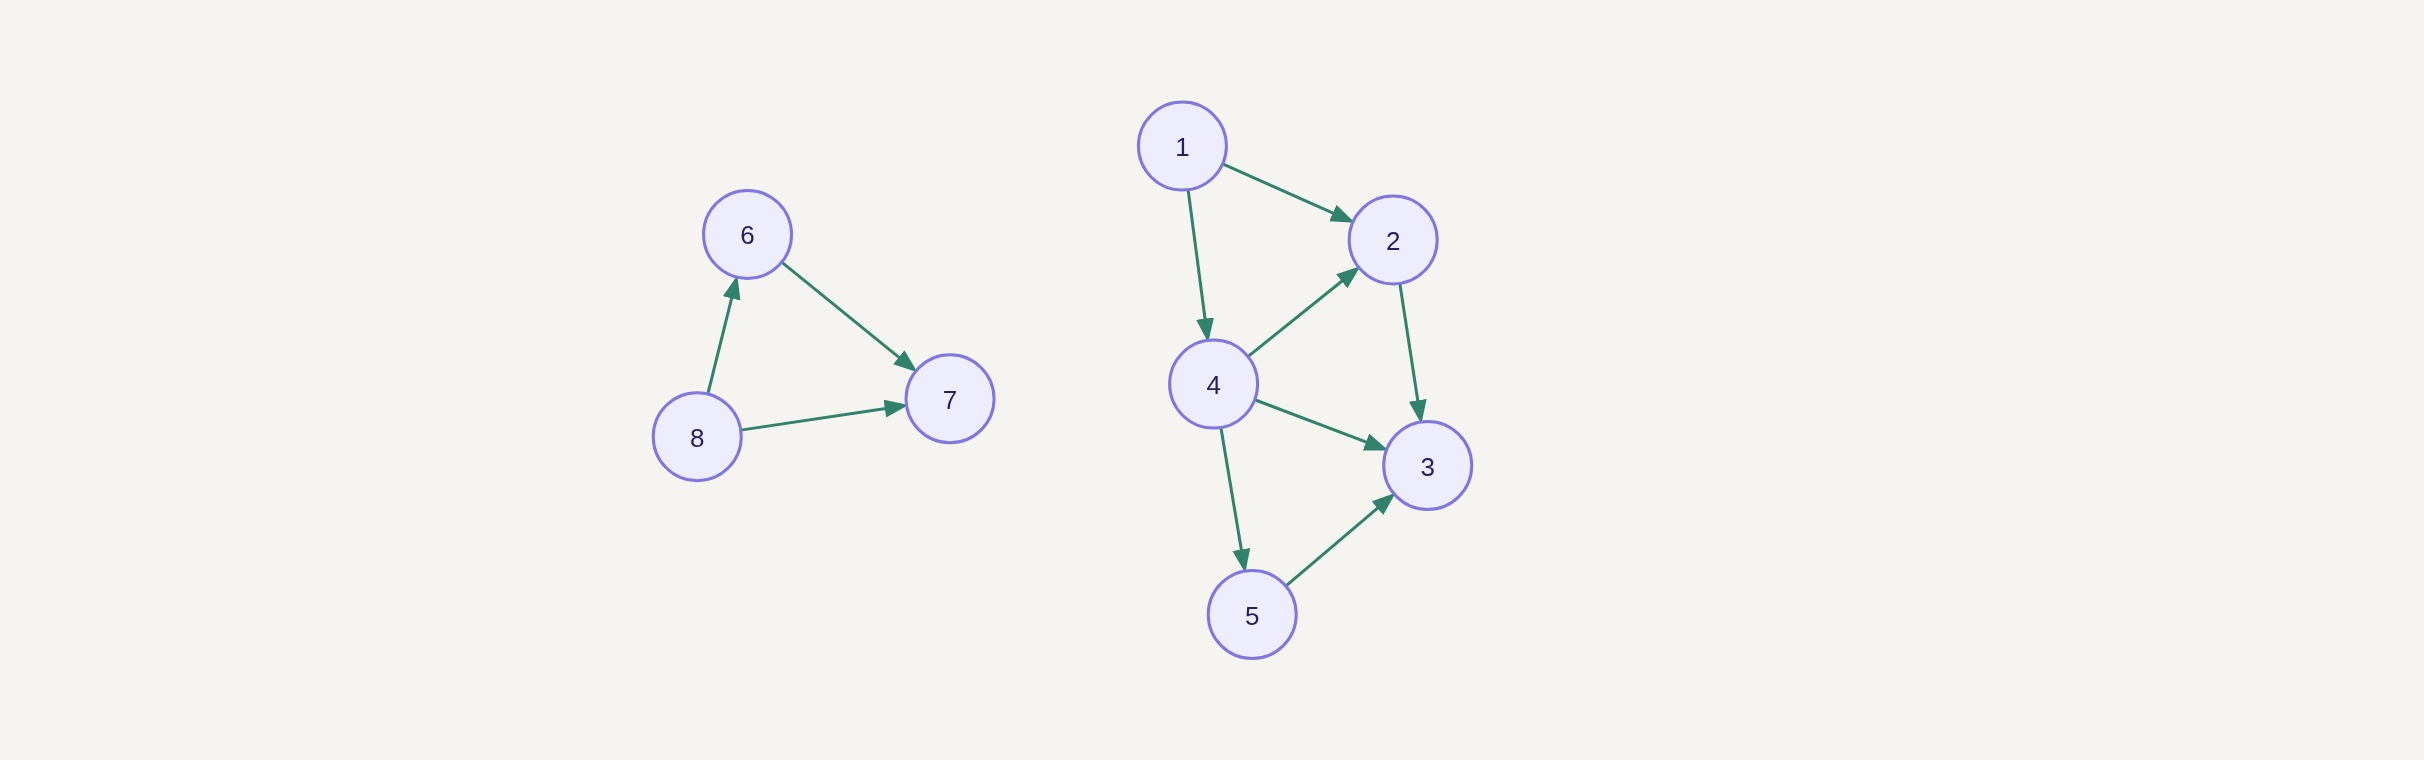
\includegraphics[scale=0.3,angle=0]{graph1.jpg}
\captionsetup{labelformat=empty}
\caption{ A graph corresponding to $g_1$ }
\end{center}
\end{figure}

\begin{align}
%\begin{matrix}
g_2 = 
\left[\begin{array}{rrrrrrrr}
0 &0 &0 &-1 &0 &0 &0 &1 \\ 
0 &0 &-1 &0 &1 &1 &1 &0 \\ 
0 &1 &0 &0 &1 &0 &0 &0 \\ 
1 &0 &0 &0 &0 &0 &0 &1 \\ 
0 &-1 &-1 &0 &0 &0 &1 &0 \\ 
0 &-1 &0 &0 &0 &0 &1 &0 \\ 
0 &-1 &0 &0 &-1 &-1 &0 &0 \\ 
-1 &0 &0 &-1 &0 &0 &0 &0 
%\end{matrix}
\end{array}\right]
\end{align}

\begin{figure}[!htbp]
\begin{center}
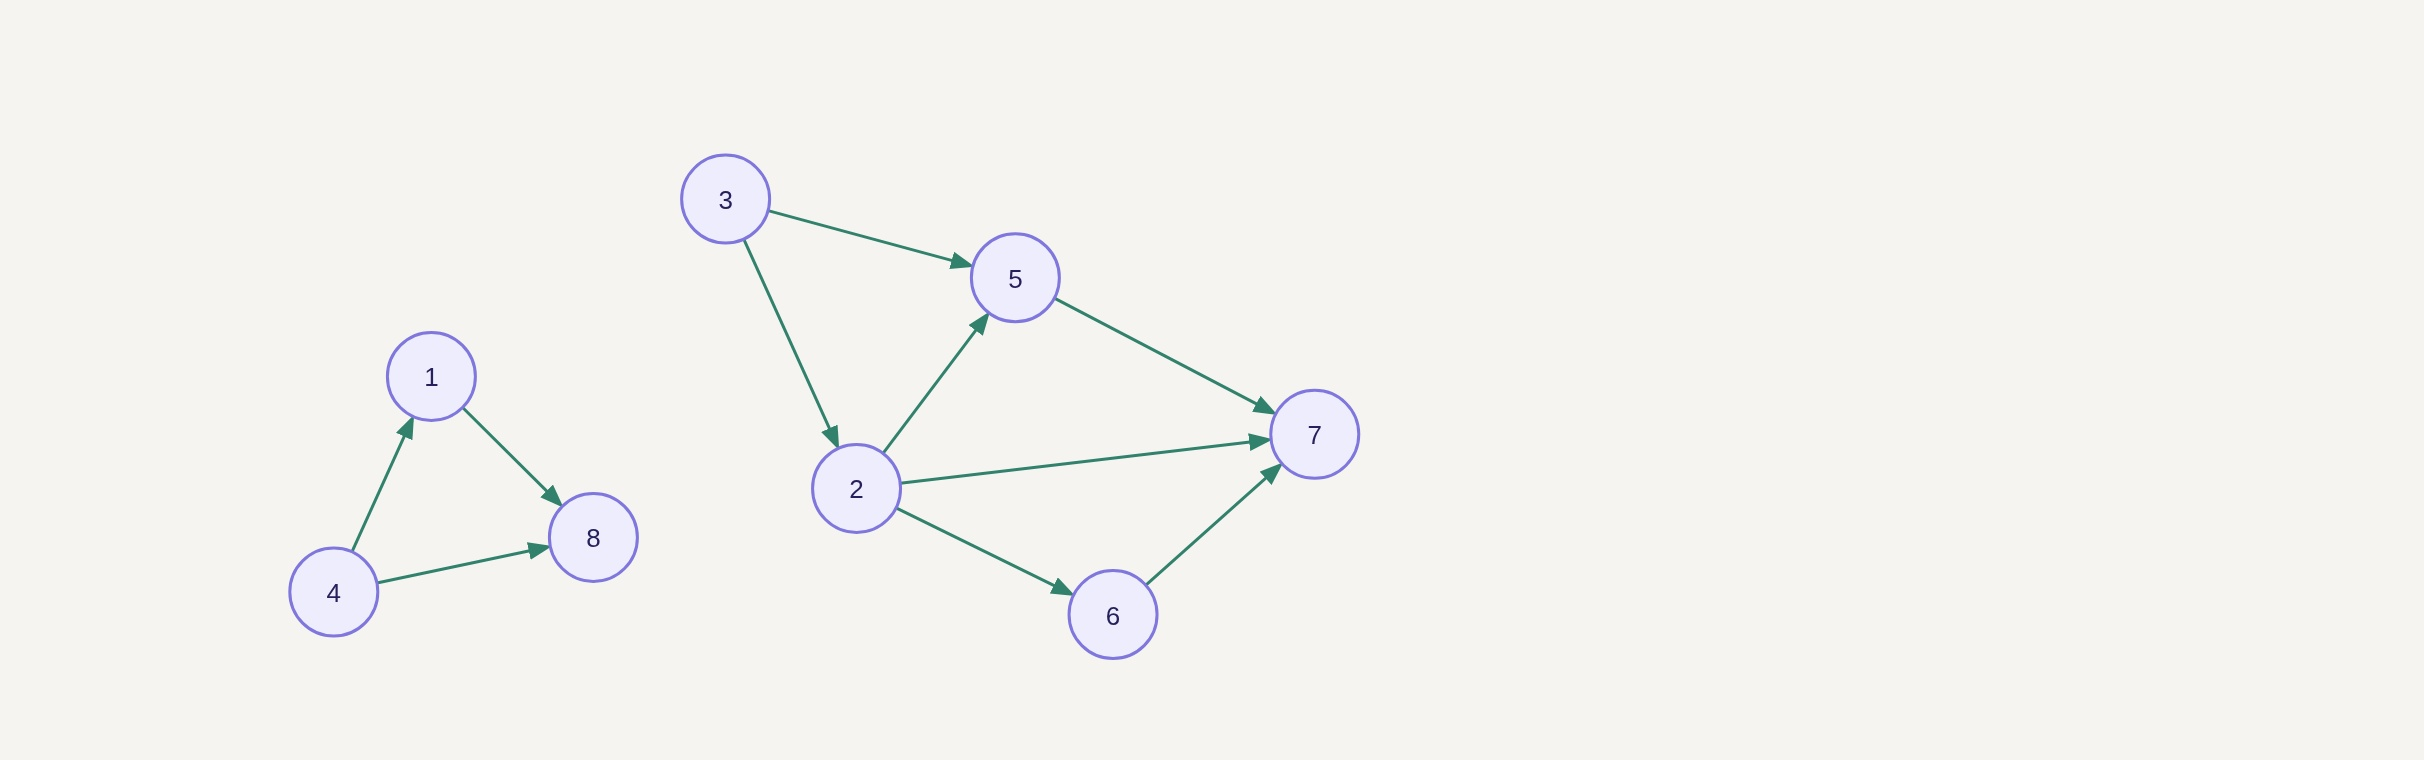
\includegraphics[scale=0.3,angle=0]{graph2.jpg}
\captionsetup{labelformat=empty}
\caption{ A graph corresponding to $g_2$ }
\end{center}
\end{figure}

\end{document}

\begin{figure}[h]
    \centering
    \subcaptionbox{Caption for A\label{fig:a}}{
        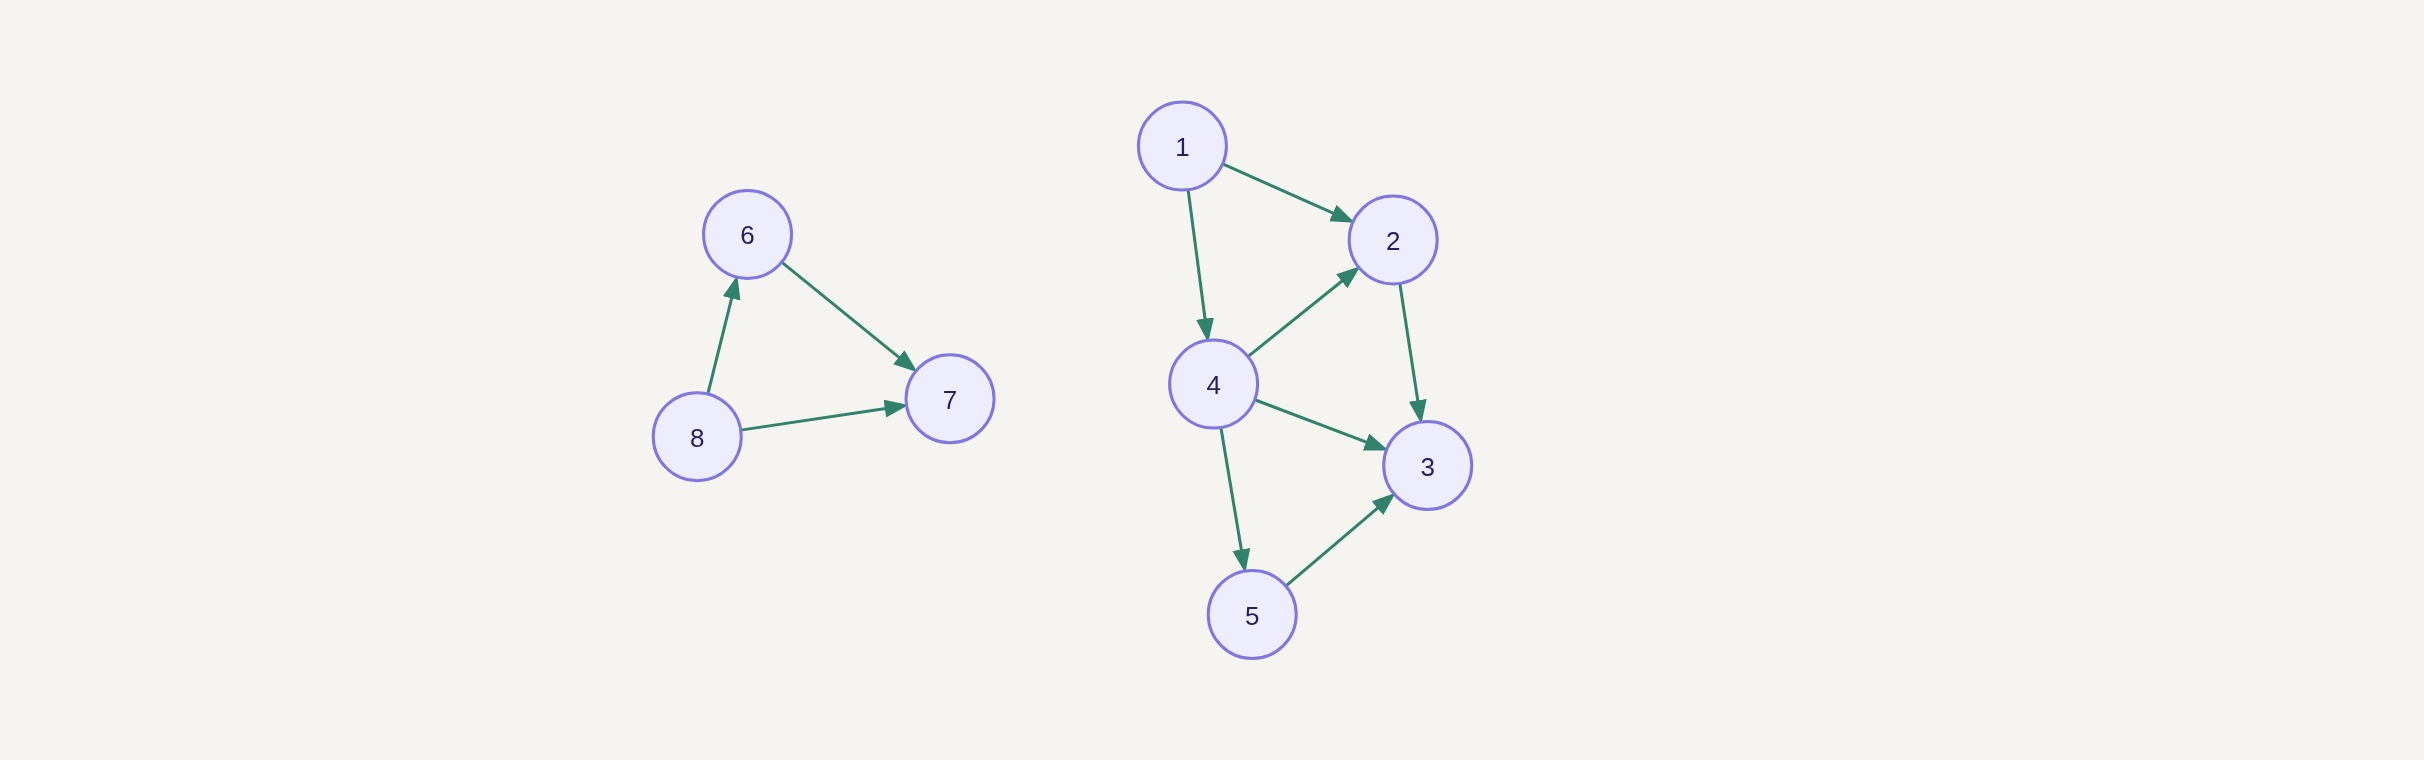
\includegraphics[width=1\textwidth]{graph1.jpg}
    }
    \hfill
    \subcaptionbox{Caption for B\label{fig:b}}{
        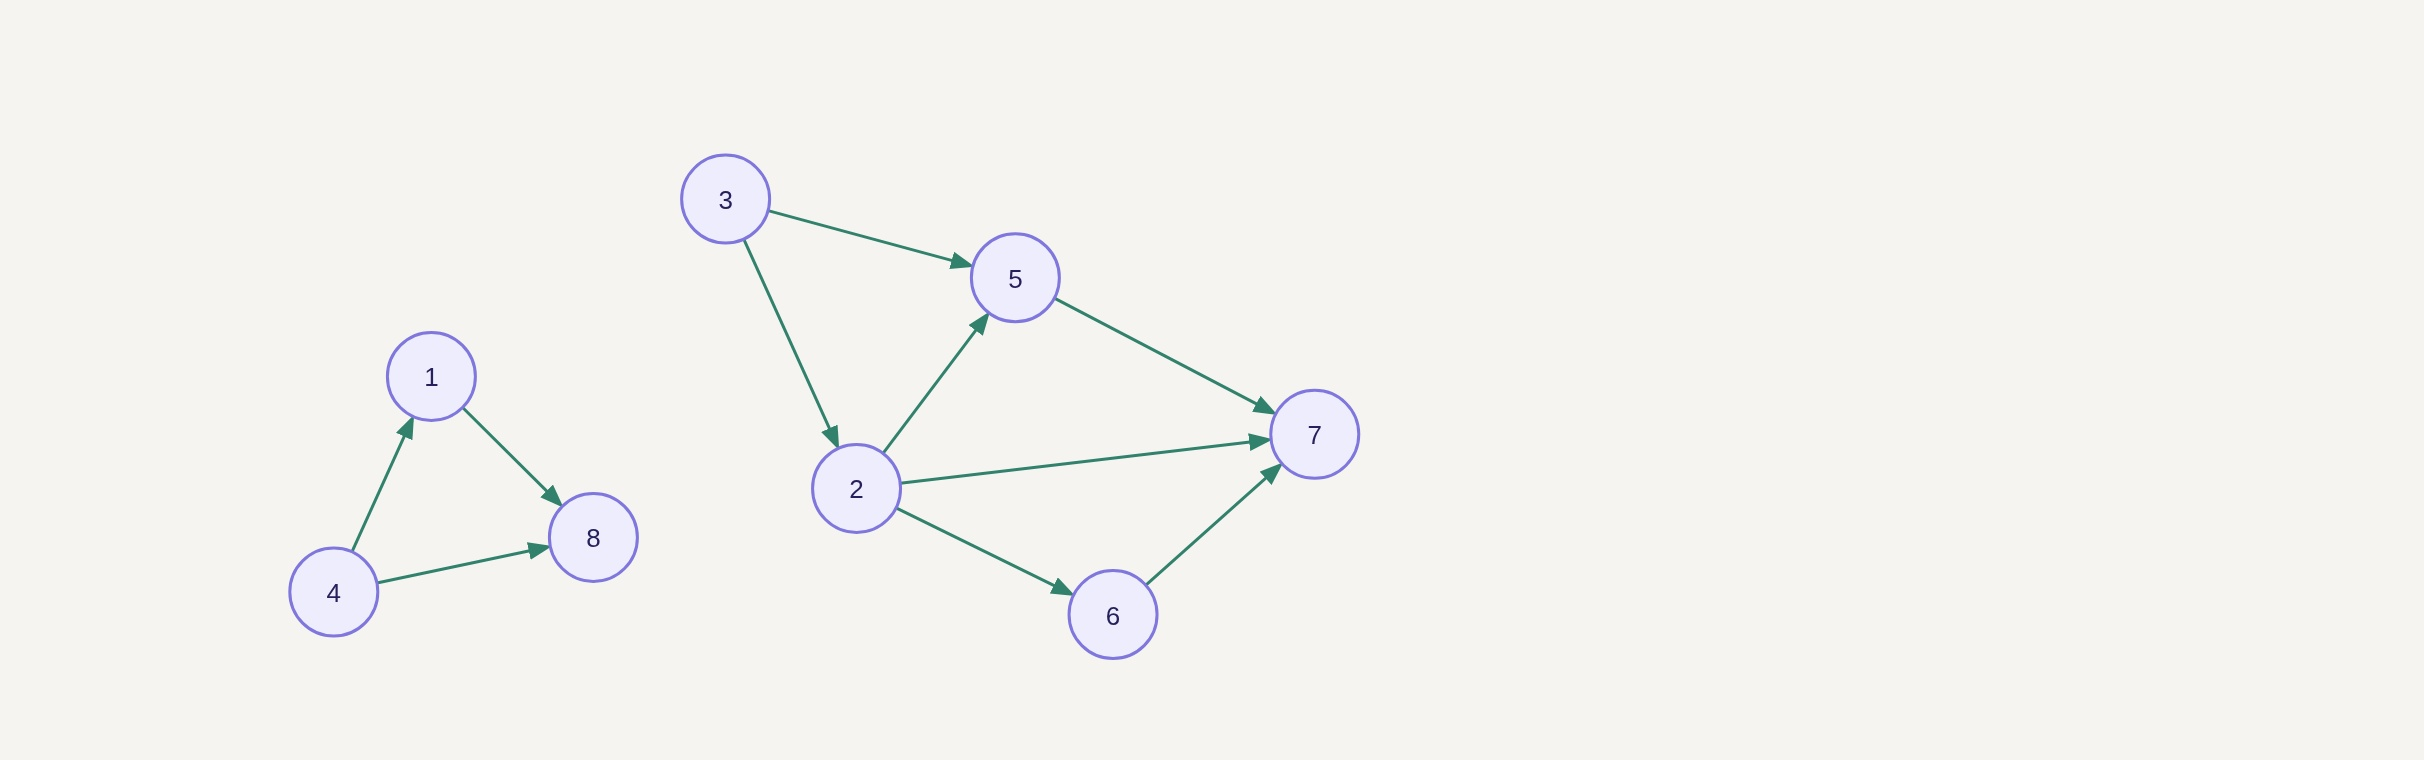
\includegraphics[width=1\textwidth]{graph2.jpg}
    }
    \caption{Overall caption}
    \label{fig:both}
\end{figure}

\begin{figure}[h]
    \centering
    \begin{minipage}{1.5\textwidth}
        \centering
        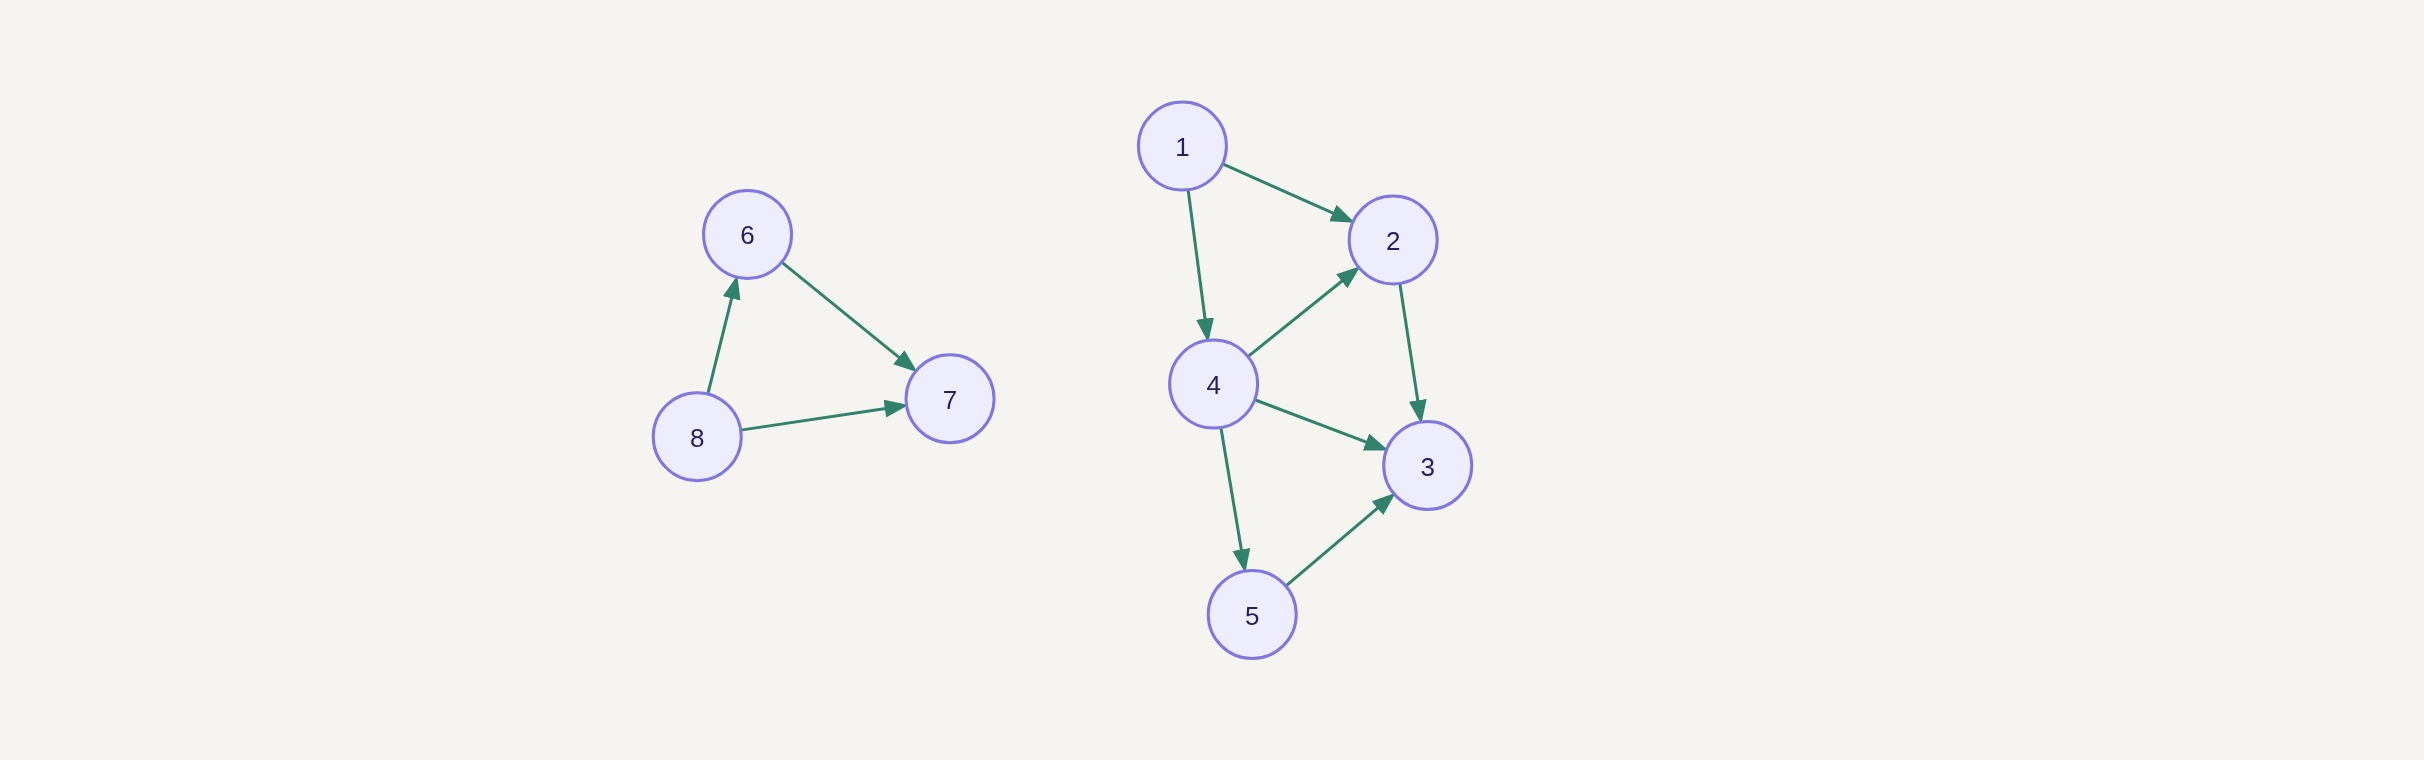
\includegraphics[width=\textwidth]{graph1.jpg}
        \caption{Caption for A}
        \label{fig:a}
    \end{minipage}
    \vfill
    \begin{minipage}{1.5\textwidth}
        \centering
        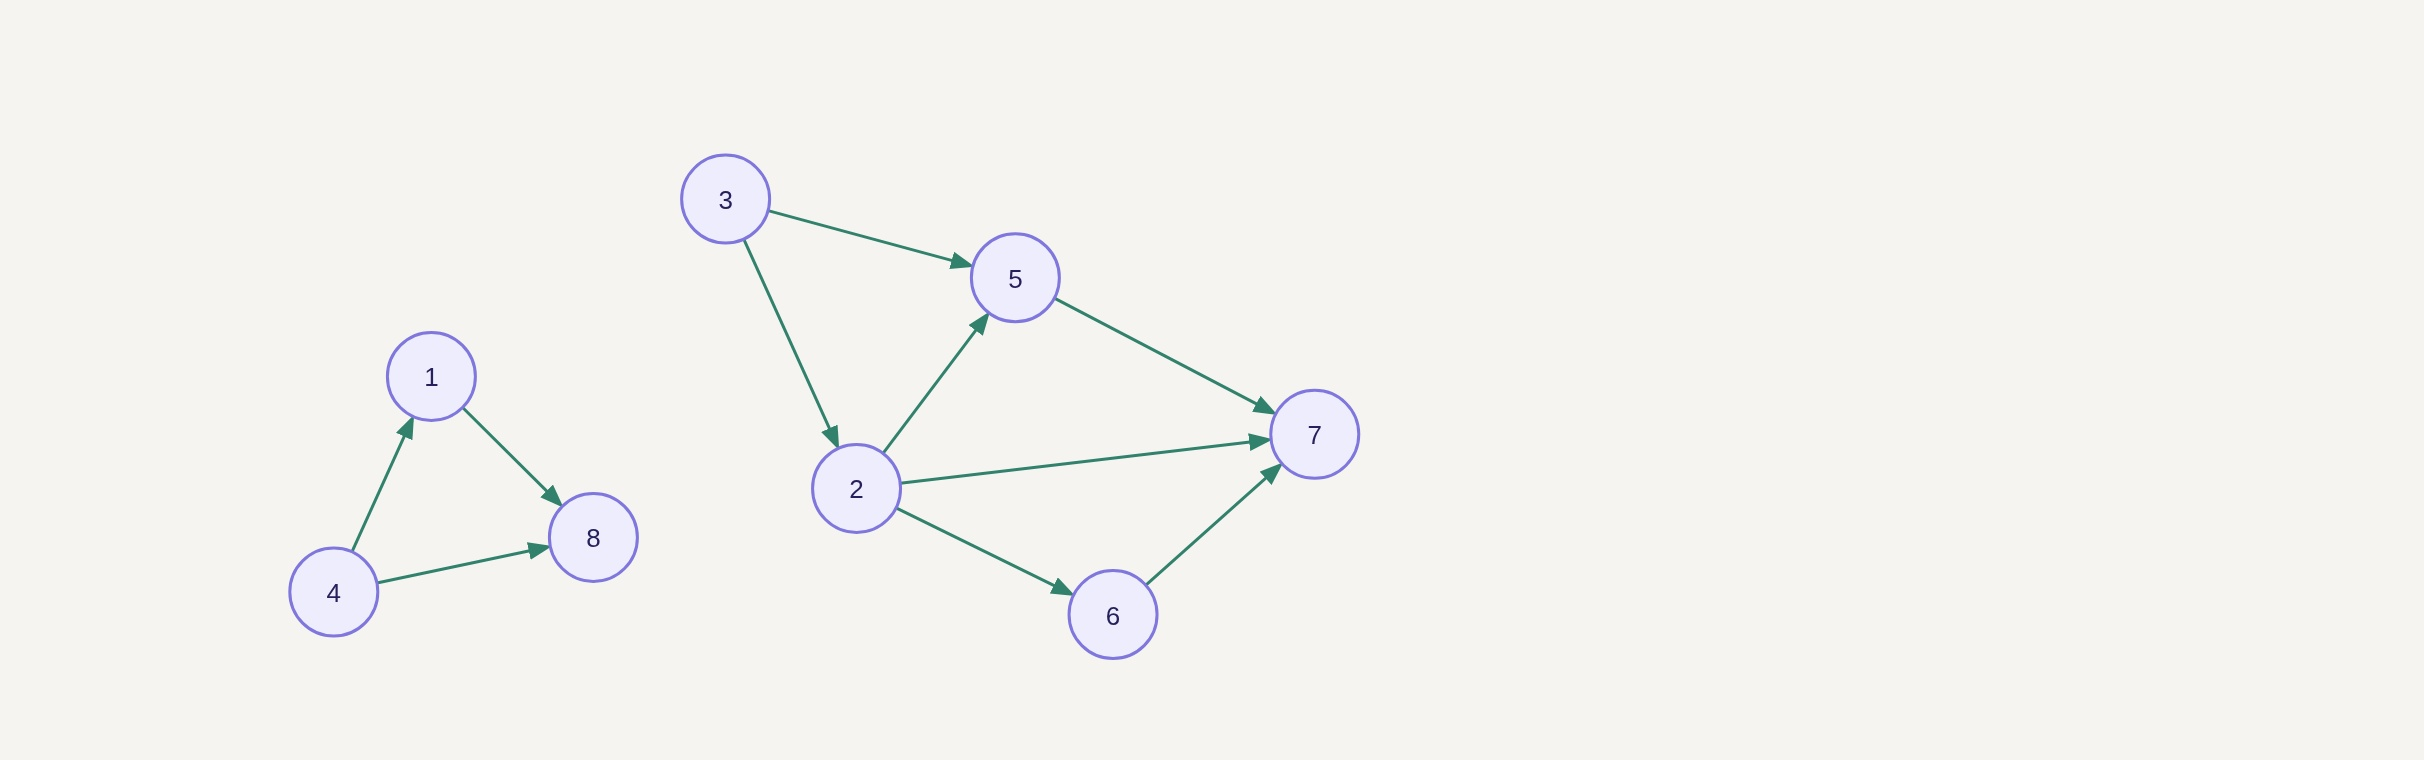
\includegraphics[width=\textwidth]{graph2.jpg}
        \caption{Caption for B}
        \label{fig:b}
    \end{minipage}
\end{figure}
\end{document}
%\begin{figure}[!htbp]
%\includegraphics[scale=0.15,angle=-90]{Images/IMG_1501.JPG}
%\captionsetup{labelformat=empty}
%\caption{ Problem s: page 1}
%\end{figure}
\begin{itemize}

\item[]
\begin{align} \begin{aligned} & \sup _{u \neq 0} \frac{\|G u\|
_{p}}{\|u\|_{p}} \equiv\|G\|_{p} \\ & \Rightarrow \forall u:\|G u\|
_{p} \leq\|G\|_{p}\left\|u_{p}\right\|\end{aligned} \end{align}

\item[ Alternately ]
\begin{align} \mbox{Let} \pr u=\underbrace{\left\lfloor\frac{1}{\sqrt{n}}
\cdots \frac{1}{\sqrt{n}}\right\rfloor}_{n} \end{align}

\item[]
\begin{align} \begin{aligned} V: & V^{\top} u=e_{1}, A=\Sigma
V^{\top} \\ \Rightarrow & \frac{|A u|_{2}}{|u|_{2}}=\sigma_{1}
=\|A\|_{2} \\ & \frac{|A u|_{\infty}}{|u|_{\infty}}=\sqrt{n}
\sigma_{1}\end{aligned} \end{align}

\item[]
\begin{align} \Rightarrow\|A\|_{2} \leq\|A\|_{\infty} \end{align}
\end{itemize}

\begin{minted}[fontsize=\footnotesize]{julia}
\end{minted}

\newpage

\setcounter{equation}{0} 
\paragraph{ y-axis symmetry of eigenvalues of a Hamiltonian}

\end{document}

\newpage
\newpage
\paragraph{}

\newpage

\begin{minted}[fontsize=\footnotesize]{julia}
350:


duty: AVG((v(m))/4)=0.434407 FROM 0 TO 8e-05
vout: AVG(v(out))=24.001 FROM 0 TO 8e-05
vs: MAX(v(s1))=621.529 FROM 0 TO 8e-05
pg: AVG(-v(in)*i(vg))=619.187 FROM 0 TO 8e-05
pout: AVG(v(out)*v(out)/rload)=576.056 FROM 0 TO 8e-05
efficiency: pout/pg=0.930344
ploss: pg-pout=43.1303
qconverter: pout/ploss=13.3562

Total elapsed time: 19.689 seconds.


270:

duty: AVG((v(m))/4)=0.568289 FROM 0 TO 8e-05
vout: AVG(v(out))=23.9995 FROM 0 TO 8e-05
vs: MAX(v(s1))=621.057 FROM 0 TO 8e-05
pg: AVG(-v(in)*i(vg))=619.518 FROM 0 TO 8e-05
pout: AVG(v(out)*v(out)/rload)=575.981 FROM 0 TO 8e-05
efficiency: pout/pg=0.929724
ploss: pg-pout=43.5374
qconverter: pout/ploss=13.2296

\end{minted}

\newpage

\begin{minted}[fontsize=\footnotesize]{julia}

fs   = 250.e3
Ctot = 2 * 750e-12 + 400e-12

Vo  = 24.
R   = 1

Vgm = 270.
Vgp = 350.


### transformer 1:n turns == 1/N
frN(N) = 1/N;

fDmax( N )  =  Vo / Vgm * N
fDmin( N )  =  Vo / Vgp * N
fD( N, Vg ) =  Vo / Vg  * N


fM( N, D )     = frN(N) * D
fMs( D )       = 1 / ( 1 - D )
fJ( N, L, Vg ) = fD( N, Vg )  * fR0( L )  / R


fF0( L ) = 1 / 2 / pi * 1 / sqrt( L * Ctot ) 
fF( L )  = fs / fF0( L ) 
fR0( L ) = sqrt( L / Ctot ) 


### Voltage stress
fVS( Vg, N ) = Vg / ( 1 - fD( N, Vg )  )

# N = 5
#plot( fVS.( 270:350, 5 ) )

## ZVS functions 
ffZVS( D, L )    =  D * sqrt( pi^2 / fF(L)^2  + fMs( D )^2 )
fgZVS( N, D, L ) = frN( N )^2  * fR0( L ) / R * D + 1

# L = 30e-5
#plot( ffZVS.( fD.( N, 270:350 ) , L ), label="ff" )
#plot!( fgZVS.( N, fD.( N, 270:350 ) , L ), label="fg" )

### Angles 

fJ( N, L, Vg ) = fD( N, Vg ) * fR0( L )  / R


fJmu3( N, L, Vg ) =  pi * fD(N,Vg) / fF(L)
fJmu2( N, L, Vg ) = sqrt( fMs( fD(N,Vg) )^2 + fJmu3( N,L,Vg)^2 )


fBeta( N, L, Vg )  = asin( fMs( fD( N, Vg ) ) / fJmu2( N, L, Vg ) )
fGamma( N, L, Vg ) =  asin( 1 / ( fJmu2( N, L, Vg ) - fJ(N,L,Vg) ) ) 
fAlpha( N, L, Vg ) = asin( (fJmu2( N,L,Vg ) + fJ(N,L,Vg) )^(-1) ) 


fSum( N, L, Vg )   = max( fBeta( N, L, Vg )  + 
		fGamma( N, L, Vg ), fAlpha( N, L, Vg ) + fBeta( N, L, Vg ) )
#julia> plot( 270:350, (fSum.( N, L, 270:350 ) / 2 / pi * 1 / fF0( L )) *1e9, label="dead time ns" )
#julia> savefig("dead time calc vs voltage ")
#"/home/andrei/Courses/ColoradoBoulder/ColoradoPE/SoftSw5447/Hw8/dead time calc vs voltage .png"

#julia> fSum.( N, L, 270 ) / 2 / pi * 1 / fF0( L )
#2-element Vector{Float64}:
# 1.3565366020654344e-7
# 1.4280221468751554e-7

#julia> fSum.( N, L, 350 ) / 2 / pi * 1 / fF0( L )
#2-element Vector{Float64}:
# 1.3775988541910618e-7
# 1.4702711062256033e-7

\end{minted}

\end{document}

\newpage
\newpage


 
 


\newpage
\newpage

\begin{minted}[fontsize=\footnotesize]{julia}

\end{minted}

\paragraph{} 


\newpage
\newpage


\begin{figure}[!htbp]
\includegraphics[scale=0.3,angle=0]{circuit.png}
\captionsetup{labelformat=empty}
\caption{ Problem s: }
\end{figure}
 
\begin{figure}[!htbp]
\includegraphics[scale=0.3,angle=0]{zvsP2.png}
\captionsetup{labelformat=empty}
\caption{ Problem s: }
\end{figure}



\end{document}

\paragraph{}


\end{document}

\paragraph{ Problem 1 } 




\newpage
\paragraph{ Problem 2 }

%\begin{figure}[!htbp]
%\includegraphics[scale=0.15,angle=-90]{Images/IMG_0943.JPG}
%\captionsetup{labelformat=empty}
%\caption{ Problem s: page 5 blank}
%\end{figure}







\newpage
\paragraph{ Problem 3}


\paragraph{}

\newpage
\newpage

\begin{minted}[fontsize=\footnotesize]{julia}

fs = 100e3

Vg = 28
V  = 48

P = 150

d   =Vg / V
dpr = 1-d

R = V^2 / P

Il = Vg / R * 1 / d^2

Imx = Il * ( 1 + 0.1 )

L = 1/2 * d * dpr^2 * 10 * R / fs
println( " L ", L ) 

# power check 
println( " Pin = 150 ? ", Il * Vg ) 


Bmx = 0.225
Ku = 0.5


rho = 1.724e-6 # Ohm cm 
mu0 = 4 * pi * 1e-7 # metric

Pl = 5e-3 * P 
Rl = Pl / Il^2 

Kg_min = rho * ( L^2 * Imx^2 / Bmx^2 ) * 1e8  / Rl / Ku # in cm^5
println( " Kg_min in cm^5 ", Kg_min ) 

fKg( Ac, Wa, mlt ) = Ac^2 * Wa / mlt

# PQ26 / 20

Ac = 1.19
Wa = 0.333
mlt = 5.62 

Kg = fKg( 1.19, 0.333, 5.62  )
println( "PQ26/20 Kg ", Kg, " Kg_min ", Kg_min ) 

Ac = 1.19 # cm^2
Wa = 0.333 # cm^2 
mlt = 5.62 # cm

n = round( L * Imx  / Bmx * 1e4 / Ac ) + 1
println( " turn count - rounded up ", n )

lg = mu0 * Ac * 1e-4 * n^2 / L

println( "lg in mm ", lg * 1e3 )

println( "wire x-section area in cm^2 ", Ku * Wa / n  )

\end{minted}


\begin{minted}[fontsize=\footnotesize]{julia}

julia> include("p3.jl")
 L 7.777777777777777e-5
 Pin = 150 ? 149.99999999999997
 Kg_min in cm^5 0.054748257327622354
PQ26/20 Kg 0.08390770462633453 Kg_min 0.054748257327622354
 turn count - rounded up 18.0
lg in mm 0.622940124095013
wire x-section area in cm^2 0.009250000000000001

\end{minted}

\end{document}

\paragraph{}
The Bode plots were done with a Matlab script ( attached ). Forgive me. Not enough time to do by hand ( and have done a few of these as of late by hand ;) 
There might be a mistake in Zout ( pure integrator in there ... did not have time to think the implications through )

\includepdf[pages=-]{Boost_TFs.pdf}

\paragraph{ Problem 3 }

\begin{figure}[!htbp]
\includegraphics[scale=0.15,angle=-90]{Images/IMG_0953.JPG}
\captionsetup{labelformat=empty}
\caption{ Problem s: page 15}
\end{figure}
 
\begin{figure}[!htbp]
\includegraphics[scale=0.15,angle=-90]{Images/IMG_0954.JPG}
\captionsetup{labelformat=empty}
\caption{ Problem s: page 16}
\end{figure}

\paragraph{}
The higher load leads to lower DC currents and lower parasitics, so the D value is closer to the 0.6 ideal ( 2.42/4 = 0.6 vs 2.66/4 = 0.67 )

\begin{minted}[fontsize=\footnotesize]{julia}

120 Ohm load:
vout: AVG(v(out))=119.679 FROM 0.0199 TO 0.02
vc: AVG(v(vc))=2.4273 FROM 0.0199 TO 0.02

12 Ohm load:

vout: AVG(v(out))=119.693 FROM 0.0199 TO 0.02
vc: AVG(v(vc))=2.66156 FROM 0.0199 TO 0.02

\end{minted}

 
\begin{figure}[!htbp]
\includegraphics[scale=0.5,angle=0]{120OhmLoad.png}
\captionsetup{labelformat=empty}
\caption{ 120 Ohm load }
\end{figure}

 
\begin{figure}[!htbp]
\includegraphics[scale=0.5,angle=0]{12OhmLoad.png}
\captionsetup{labelformat=empty}
\caption{ 12 Ohm load }
\end{figure}


\end{document}
%\paragraph{ Problem 1 Numerical Checks }

%\newpage 

%\begin{figure}[!htbp]
%\includegraphics[scale=0.4,angle=0]{P4p6/circuitRealization.png}
%\captionsetup{labelformat=empty}
%\caption{ Problem : page 6, ltspice realization with ideal SPDT switches AND ideal diodes + an npn BJT with ideal modulators in the biasing arms}
%\end{figure}
%inductor_current_ripple.png

%\newpage


\paragraph{ Problem 2 }

%\newpage

\paragraph{ Part A }

\begin{itemize}
	\item[ DC out ] 1.0038 V average over steady state region, so within 0.5 \% of 1 V ( < 50 mV )
	\item[ Ripple ] 8.5mV, so less than 10 mV, so also meets the spec
	\item[ Total Loss ]  19 W ( from measure logs )
	\item[ Efficiency ]  84.1 \%  ( from measure logs )                                                            
\end{itemize}


\paragraph{ Part B }
\begin{itemize}
	\item[2] V(g1, sw), top gate to source voltage ( for M1 ) 
	\item[3] V(g2), bottom gate to source voltage ( for M2 ) 
	\item[4] Id(M1) top switch drain current 
	\item[5] V(out) output voltage
	\item[6] I(L1) inductor current
\end{itemize}

\paragraph{ Part C }
\begin{itemize}
	\item[B] Reverse flow region of M2, when the body diode conducts in M2, hence the switch node voltage is about 0.8 V below ground. M1 turns off, M2 is turnig on
	\item[C] same as B, but M2 is turning off, M1 is turning on. Both B and C is during dead times
	\item[D] Idk what this is: 
	\item[E] This is the reverse recovery current from the body diode of M2. Because I(L1) is continuous, this current is pulled through M1 from the the main power sources Vg. 
	M2 is turning off and M1 is turning on
	\item[F] M1 conducts for the smaller of the duties ( 0.12 ) and this is the delta associate with the main inductor current ripple
	\item[G] Peak inductor current
	\item[H] Peak output voltage displaced 90 degrees from peak inductor current ( dv/dt and di/dt are out of phase )
\end{itemize}

\paragraph{ Part D }

From the circuit there is about 19W of total loss. From DC reduction one gets about 12.9 W of conduction loss. So, in this case conduction loss is larger than switching loss
( + gate drive loss ).

\newpage 
\begin{figure}[!htbp]
\includegraphics[scale=0.1,angle=-0]{P2/P2Images/IMG_0737.JPG}
\captionsetup{labelformat=empty}
\caption{ Problem s: page 1}
\end{figure}
 
\begin{figure}[!htbp]
\includegraphics[scale=0.1,angle=-0]{P2/P2Images/IMG_0738.JPG}
\captionsetup{labelformat=empty}
\caption{ Problem s: page 2}
\end{figure}
 
\begin{figure}[!htbp]
\includegraphics[scale=0.1,angle=-0]{P2/P2Images/IMG_0739.JPG}
\captionsetup{labelformat=empty}
\caption{ Problem s: page 3}
\end{figure}
 
\begin{figure}[!htbp]
\includegraphics[scale=0.1,angle=-0]{P2/P2Images/IMG_0740.JPG}
\captionsetup{labelformat=empty}
\caption{ Problem s: page 4}
\end{figure}
 
\begin{figure}[!htbp]
\includegraphics[scale=0.1,angle=-0]{P2/P2Images/IMG_0741.JPG}
\captionsetup{labelformat=empty}
\caption{ Problem s: page 5}
\end{figure}
 
\begin{figure}[!htbp]
\includegraphics[scale=0.1,angle=-0]{P2/P2Images/IMG_0742.JPG}
\captionsetup{labelformat=empty}
\caption{ Problem s: page 6}
\end{figure}
 
\begin{figure}[!htbp]
\includegraphics[scale=0.1,angle=-0]{P2/P2Images/IMG_0743.JPG}
\captionsetup{labelformat=empty}
\caption{ Problem s: page 7}
\end{figure}
 
\begin{figure}[!htbp]
\includegraphics[scale=0.1,angle=-0]{P2/P2Images/IMG_0744.JPG}
\captionsetup{labelformat=empty}
\caption{ Problem s: page 8}
\end{figure}
 


%\paragraph{ Problem 2 Numerical Checks }

\newpage

%\begin{figure}[!htbp]
%\includegraphics[scale=0.4,angle=0]{P4p3/p4p3_spice.png}
%\captionsetup{labelformat=empty}
%\caption{ Problem : page 6, ltspice realization }
%\end{figure}
%inductor_current_ripple.png

%\begin{minted}[fontsize=\footnotesize]{julia}
%\end{minted}

\end{document}

\newpage

\paragraph{ Problem  4.1  }

%\begin{figure}[!htbp]
%\includegraphics[scale=0.15,angle=-90]{P4p1/P4p1Images/IMG_0647.JPG}
%\captionsetup{labelformat=empty}
%\caption{ Problem s: page 1}
%\end{figure}
 
%\begin{figure}[!htbp]
%\includegraphics[scale=0.15,angle=-90]{P4p1/P4p1Images/IMG_0648.JPG}
%\captionsetup{labelformat=empty}
%\caption{ Problem s: page 2}
%\end{figure}
 
\begin{figure}[!htbp]
\includegraphics[scale=0.15,angle=-90]{P4p1/P4p1Images/IMG_0649.JPG}
\captionsetup{labelformat=empty}
\caption{ Problem s: page 3}
\end{figure}
 
\begin{figure}[!htbp]
\includegraphics[scale=0.15,angle=-90]{P4p1/P4p1Images/IMG_0650.JPG}
\captionsetup{labelformat=empty}
\caption{ Problem s: page 4}
\end{figure}

\newpage
\paragraph{ Problem  4.1 Numerical Checks }
\newpage


\begin{figure}[!htbp]
\includegraphics[scale=0.25,angle=0]{P4p1/4p1_spice_realization.png}
\captionsetup{labelformat=empty}
\caption{ Problem : page 5, spice realization}
\end{figure}


\newpage
\paragraph{ Problem 2 }
 
\begin{figure}[!htbp]
\includegraphics[scale=0.15,angle=-90]{P2/P2Images/IMG_0651.JPG}
\captionsetup{labelformat=empty}
\caption{ Problem s: page 1}
\end{figure}
 
\begin{figure}[!htbp]
\includegraphics[scale=0.15,angle=-90]{P2/P2Images/IMG_0652.JPG}
\captionsetup{labelformat=empty}
\caption{ Problem s: page 2}
\end{figure}
 
\begin{figure}[!htbp]
\includegraphics[scale=0.15,angle=-90]{P2/P2Images/IMG_0653.JPG}
\captionsetup{labelformat=empty}
\caption{ Problem s: page 3}
\end{figure}
 
\begin{figure}[!htbp]
\includegraphics[scale=0.15,angle=-90]{P2/P2Images/IMG_0654.JPG}
\captionsetup{labelformat=empty}
\caption{ Problem s: page 4}
\end{figure}
 
%\begin{figure}[!htbp]
%\includegraphics[scale=0.15,angle=-90]{P2/P2Images/IMG_0655.JPG}
%\captionsetup{labelformat=empty}
%\caption{ Problem s: page 5}
%\end{figure}
 
%\begin{figure}[!htbp]
%\includegraphics[scale=0.15,angle=-90]{P2/P2Images/IMG_0656.JPG}
%\captionsetup{labelformat=empty}
%\caption{ Problem s: page 6}
%\end{figure}
 
%\begin{figure}[!htbp]
%\includegraphics[scale=0.15,angle=-90]{P2/P2Images/IMG_0657.JPG}
%\captionsetup{labelformat=empty}
%\caption{ Problem s: page 7}
%\end{figure}
 
%\begin{figure}[!htbp]
%\includegraphics[scale=0.15,angle=-90]{P2/P2Images/IMG_0658.JPG}
%\captionsetup{labelformat=empty}
%\caption{ Problem s: page 8}
%\end{figure}
 
%\begin{figure}[!htbp]
%\includegraphics[scale=0.15,angle=-90]{P2/P2Images/IMG_0659.JPG}
%\captionsetup{labelformat=empty}
%\caption{ Problem s: page 9}
%\end{figure}

\begin{figure}[!htbp]
\includegraphics[scale=0.15,angle=-90]{P2/P2ImagesTake2/IMG_0660.JPG}
\captionsetup{labelformat=empty}
\caption{ Problem 2: page 5}
\end{figure}
 
\begin{figure}[!htbp]
\includegraphics[scale=0.15,angle=-90]{P2/P2ImagesTake2/IMG_0661.JPG}
\captionsetup{labelformat=empty}
\caption{ Problem 2: page 6}
\end{figure}
 
\begin{figure}[!htbp]
\includegraphics[scale=0.15,angle=-90]{P2/P2ImagesTake2/IMG_0662.JPG}
\captionsetup{labelformat=empty}
\caption{ Problem 2: page 7}
\end{figure}
 
\begin{figure}[!htbp]
\includegraphics[scale=0.15,angle=-90]{P2/P2ImagesTake2/IMG_0663.JPG}
\captionsetup{labelformat=empty}
\caption{ Problem 2: page 8}
\end{figure}

\end{document}


\begin{figure}[!htbp]
\includegraphics[scale=0.5,angle=0]{P2/inductor_current_with_inductor_loss_plot_for_ss.png}
\captionsetup{labelformat=empty}
\caption{ Problem 2: page 10}
\end{figure}


\begin{minted}[fontsize=\footnotesize]{julia}

fMhw2p1(d,dpr, Vb, Vd, R, Rd, Ron, Rl ) = 1 ./ dpr .* 
		( 1 .- Vd / Vb * dpr ./ 1 ) * 1 ./ ( 1 .+ 1 ./ ( R * dpr^2 ) 
			.* ( dpr * Rd .+ Rl .+ d * Ron ) )

julia> d * 190e-3 * 
	( fMhw2p1( d, 1-d, 50, 0.6, 100, 0.06, 190e-3, 0.5 ) / ( 1 - d ) * Vg/100 )^2
7.4217001221744

julia> fMhw2p1( d, 1-d, 50, 0.6, 100, 0.06, 190e-3, 0.5 ) *  ( 1 - d )
0.9020991675714803

julia> fMhw2p1( d, 1-d, 50, 0.6, 100, 0.06, 190e-3, 0.5 ) / ( 1 - d ) * Vg/100
7.216793340571843

julia> fMhw2p1( d, 1-d, 50, 0.6, 100, 0.06, 190e-3, 0.5 ) 
3.6083966702859214

\end{minted}


\begin{minted}[fontsize=\footnotesize]{julia}
.meas PM1 avg(-v(sw)*id(m1)) from 1.9m
.meas M avg(v(out))/v(in) from 1.9m
\end{minted}
 

\end{document}

\paragraph{}

For part B ( but see plots ): 
The values from spice are: 188 V ( 0.6 V ripple p-p ), 8.3 A ( 7.3 A ripple p-p ). Average voltate is close, ave current is within 2 A, ripple is within an amp, voltage 
ripple is off ( by about 0.3 V out of 0.6 ) 

\paragraph{} 
Average output power is 356 W vs ave input of 415 W, so 0.86 efficiency 


\newpage


\paragraph{ Problem  2 Numerical Checks }


\begin{figure}[!htbp]
\includegraphics[scale=0.5,angle=0]{P2/inductor_current_ripple.png}
\captionsetup{labelformat=empty}
\caption{ Problem 2: page 9}
\end{figure}
%inductor_current_ripple.png

\begin{figure}[!htbp]
\includegraphics[scale=0.5,angle=0]{P2/boost_with_inductor_loss_plot_for_ss.png}
\captionsetup{labelformat=empty}
\caption{ Problem 2: page 10}
\end{figure}


\begin{figure}[!htbp]
\includegraphics[scale=0.5,angle=0]{P2/inductor_current_with_inductor_loss_plot_for_ss.png}
\captionsetup{labelformat=empty}
\caption{ Problem 2: page 10}
\end{figure}

\begin{minted}[fontsize=\footnotesize]{julia}
using VMLS, LinearAlgebra

N = 2

Rl = 0.5 
R  = 100

L1 = 47e-6
C1 = 22e-6

L2 = -1
C2 = -1

vg = 50

tau = 1 / 100e3

fA1( L1, L2, C1, C2, R ) = [ [-Rl/L1 0]; [0 -1/R/C1 ]; ];
fA2( L1, L2, C1, C2, R ) = [ [-Rl/L1 -1/L1]; [1/C1 -1/R/C1 ]; ];

A1 = fA1( L1, L2, C1, C2, R )
A2 = fA2( L1, L2, C1, C2, R )

fvg( vg, L1 )  = [ vg/L1 0 ]';
vvg = -fvg( vg, L1 ) 

vs1 = inv(A1) * vvg
vs2 = inv(A2) * vvg

feA1(d, tau)  = exp( A1 * (d) * tau )       #   S closed
feA2(d, tau)  = exp( A2 * (1-d) * tau )     #   S open

\end{minted}

\newpage


\paragraph{ Problem 3} 

\begin{figure}[!htbp]
\includegraphics[scale=0.15,angle=-90]{P3Images/IMG_0618.JPG}
\captionsetup{labelformat=empty}
\caption{ Problem s: page 1}
\end{figure}
 
\begin{figure}[!htbp]
\includegraphics[scale=0.15,angle=-90]{P3Images/IMG_0619.JPG}
\captionsetup{labelformat=empty}
\caption{ Problem s: page 2}
\end{figure}
 
\begin{figure}[!htbp]
\includegraphics[scale=0.15,angle=-90]{P3Images/IMG_0620.JPG}
\captionsetup{labelformat=empty}
\caption{ Problem s: page 3}
\end{figure}



\newpage 

\paragraph{ Problem 3 Numerical Checks }

 
\begin{figure}[!htbp]
\includegraphics[scale=0.4,angle=0]{P3/vRvg.png}
\captionsetup{labelformat=empty}
\caption{ Problem s: page 3}
\end{figure}

\begin{minted}[fontsize=\footnotesize]{julia}
N = 2

L1 = 10e-6
C1 = 100e-6
R = 1

L2 = -1
C2 = -1

vg = 100

tau = 1 / 250e3

fA1( L1, L2, C1, C2, R ) = [ [0 -1/L1]; [1/C1 -1/R/C1 ]; ];
fA2( L1, L2, C1, C2, R ) = [ [0 -1/L1]; [1/C1 -1/R/C1 ]; ];

A1 = fA1( L1, L2, C1, C2, R )
A2 = fA2( L1, L2, C1, C2, R )

fvg( vg, L1 )  = [ vg/L1 0 ]';
vvg = -fvg( vg, L1 ) 

vs1 = inv(A1) * vvg
vs2 = -inv(A2) * vvg

feA1(d, tau)  = exp( A1 * (d) * tau )       #   pos 1 duty
feA2(d, tau)  = exp( A2 * (1-d) * tau )     #   pos 2 duty
\end{minted}

\newpage

\paragraph{ Problem 4 } 
 
\begin{figure}[!htbp]
\includegraphics[scale=0.15,angle=-90]{P4images/IMG_0621.JPG}
\captionsetup{labelformat=empty}
\caption{ Problem 4: page 1}
\end{figure}
 
\begin{figure}[!htbp]
\includegraphics[scale=0.15,angle=-90]{P4images/IMG_0622.JPG}
\captionsetup{labelformat=empty}
\caption{ Problem 4: page 2}
\end{figure}
 
\begin{figure}[!htbp]
\includegraphics[scale=0.15,angle=-90]{P4images/IMG_0623.JPG}
\captionsetup{labelformat=empty}
\caption{ Problem 4: page 3}
\end{figure}
 
\begin{figure}[!htbp]
\includegraphics[scale=0.15,angle=-90]{P4images/IMG_0624.JPG}
\captionsetup{labelformat=empty}
\caption{ Problem 4: page 4}
\end{figure}

\newpage
\paragraph{ Problem 4 Numerical Checks }

\begin{figure}[!htbp]
\includegraphics[scale=0.4,angle=0]{P4/dc_currents.png}
\captionsetup{labelformat=empty}
\caption{ Problem 4: page 5}
\end{figure}


\begin{figure}[!htbp]
\includegraphics[scale=0.4,angle=0]{P4/dc_value_spice.png}
\captionsetup{labelformat=empty}
\caption{ Problem 4: page 6}
\end{figure}


\begin{figure}[!htbp]
\includegraphics[scale=0.4,angle=0]{P4/voltage_ripple.png}
\captionsetup{labelformat=empty}
\caption{ Problem 4: page 6}
\end{figure}

\newpage
\begin{minted}[fontsize=\footnotesize]{julia}
N = 4 

L1 = 100e-6
C1 = 10e-5

L2 = 1e-4
C2 = 1e-4

R = 10

vg = 100

tau = 1 / 400e3

fA1( L1, L2, C1, C2, R ) = [ [0 0 -1/L1 0]; [ 0 0 0 -1/L2]; [1/C1 0 0 0]; [0 1/C2 0  -1/R/C2]; ];
fA2( L1, L2, C1, C2, R ) = [ [0 0 -1/L1 0]; [ 0 0 1/L2 -1/L2]; [1/C1 -1/C1 0 0]; [0 1/C2 0 -1/R/C2]; ];

A1 = fA1( L1, L2, C1, C2, R )
A2 = fA2( L1, L2, C1, C2, R )

fvg( vg, L1 )  = [ vg/L1 0 0 0 ]';
vvg = -fvg( vg, L1 ) 

vs1 = inv(A1) * vvg
vs2 = inv(A2) * vvg

feA1(d, tau)  = exp( A1 * (1-d) * tau ) #   open switch duty
feA2(d, tau)  = exp( A2 * d * tau )     #   closed switch duty
\end{minted}

\end{document} 


\newpage
\paragraph{ Bonus Problem }


\newpage

\paragraph{ Bonus Problem:  Numerical Checks }

%\includepdf[pages=-]{PBonus_Hw7.pdf}


\end{document}



\paragraph{ Problem 1 }

\begin{itemize}
\item[A] 
Consider a dyad decomposition of $A = V D V^{-1} \equiv V D W $ where $V$ is a matrix of known eigenvalues and $W=V^{-1}$. One has 
\begin{eqnarray*}
  	A &=& V D W, D = W A V, A^{-1} = V D^{-1} W \\ 
    A &=& \sum_i \lambda_i V_{*,i} W_{i,*} 
\end{eqnarray*}
The last line can also be rewritten if the dyads are extended into column vectors of length $N^2$ via $reshape(  V_{*,i} W_{i,*} , N^2, 1 $
and the right hand side becomes a columen vector of stacked columns of $A_m$, then we are looking for a least squares solution of 
\begin{equation}
 \min \| [ vec(  V_{*,1} W_{1,*} )  vec(  V_{*,1} W_{1,*} ) ...  vec(  V_{*,N} W_{N,*} )]  \bar{\lambda} - vec( A_m ) \|
\end{equation}

Once the best fit eigenvalues are found the estimate matrix is formed as $ \hat{A} =V D(\bar{\lambda_{ls}}) W $
\subitem Exact minimizer because of the BLUE property of least squares? 

\item[B] see code. $J = 0.0174$

\end{itemize}


\paragraph{ Problem 2 }
\begin{itemize}
\item[A]
	\subitem [if] 
	If f(x) can be expressed as 
	$\| F x \|^2$, then $ x^T A x = x^T F^T F x = x^T V \Sigma U^T U \Sigma V^T x = x^T V \Sigma^2 V^T x = \sum_i q_i^2 \sigma_i^2 \ge 0 $ with 
  $ q \equiv V^T x $

	\subitem [and only if]
	If f(x) is positive semi definite, then: because A is symmetric, it admits a decomposition in the form $ Q^T D Q $ ( for full rank, or non-full rank 
	square cases ). Then, $ x^T Q^T D Q x = q^T D q = \sum_i d_i q_i^2 $, we can always chose an x, or q as $e_i$ which would make every $d_i$ non-negative
	because here we start with positive semi-definite assumption. This in turns means that there is a square root of D, then $F = \sqrt{D} Q$

	\subitem [smallest F] smallest F, or smmallest rank of F is rank of A ... 


\item[B] 
	Another way of phrasing the question is: prove that sum of two positive semi-definite matrices is also positive semidefinite. 
	Let A and B be psd. Then each quadratic form ( per part A ) is expressible as $\| F x \|^2$ and $\| G x \|^2$ respectively. Then 
  $ x^T ( A + B ) x  = x^T F^T F x + x^T G^T G x $ and therefore the sum will be also psd. Which in turn means, that 
  $ \| C x \|^2 \equiv x^T ( A + B ) x $ and  
  $ \| C x \|^2 - \| G x \|^2 = x^T A x $
	\subitem $B_1$
		How small can the sizes of F and G be? Not sure here ... I believe one of the two can have a rank smaller than the needed rank of the sum ( down to 0 ) 
\end{itemize}

\paragraph{ Problem 3 }
\begin{itemize}
 \item[A] 
	The algorithm has the following steps:
	\subitem A.1  Form $A$, so that $h = A w$
	\subitem A.2  Form $C$ which projects $h$ onto the range of interest $ n+1 \pm k $: $ h_p = C A w $
	\subitem A.3 Maximize $\frac{ w^T A^T  C^T C A w }{w^T A^T A w } $ as follows: 
		\begin{eqnarray*}
			v^T v &=& w^T A^T A w  \\
			v^T B^T B v &=& w^T A^T  C^T C A w  \\
			v^T B^T B v &=& v^T X^T A^T  C^T C A X v \\
			v^T v &=& v^T X^T A^T A X v \\
      X^T A^T A X &=& I, X = (A^T A)^{-\frac{1}{2}}  \\
			B &=& C A (A^T A)^{-\frac{1}{2}}
		\end{eqnarray*}
		Max svd vector of $B$, can then be solved for $w$ as $ w = X v_{mx, svd}$
%	\subitem A.3  Minimize $ w^T A^T A w - w^T A^T C^T C A w  =  w^T A^T ( I - C^T C ) A w =  1 - \frac{ w^T A^T  C^T C A w }{w^T A^T A w } $. 
%	\subitem A.4  $A^T ( I - C^T C ) A$ is still positive-definite and smallest eigenvalue direction should minimize the quadratic form

	The matrices $A_{2n-1,n}$ and $C $ have the following form: 
	\begin{eqnarray*}
	A &=& 
	\begin{bmatrix}
		c_1 & 0_{1,n-1} \\
		c_2 & c_1 & 0_{1,n-2}  \\
		c_3 & c_2 & c_1 & 0_{1,n-3} \\
		.. \\
    c_n & c_{n-1} & c_{n-2} & c_{n-3} &.. & c_1 \\
    0_{1,1} & c_n & c_{n-1} & c_{n-2} & .. & c_2   \\ 
    0_{1,2} & & c_n  & c_{n-1} &  ..& c_3 \\
    .. \\
    0_{1,n-1} & & & & & c_n 
	\end{bmatrix} \\ 
	C_{2k+1,2N-1} &=& 
	%[ 0_{1,n-k} 1_{1,k} 1_{1,1} 1_{1,k} 0_{1,n-k-2} ]^T [ 0_{1,n-k} 1_{1,k} 1_{1,1} 1_{1,k} 0_{1,n-k-2} ] - I_{2n-1,2n-1}
	\begin{bmatrix}
	0_{1,n-k} & 1 & 0_{1,n+k-2} \\
	0_{1,n-k} & 0 & 1 & 0_{1,n+k-1} \\
	... \\
	0_{1,n-k} & 0_{1,2k} & 1 & 0_{1,n-k-2} \\
	\end{bmatrix}
	\end{eqnarray*}

	\item[B]
DTE is 0.93

\begin{figure}[h]
\includegraphics[scale=0.5]{"p3b_w.png"}
\includegraphics[scale=0.5]{"p3b_Aw.png"}
\caption{Problem 3: Equalized response and w input for max concentration }
\end{figure}
	
\end{itemize}

\paragraph{ Problem 4 }


%\caption{Problem 3: Equalizer and response h }

\paragraph{ Problem 5} 

\begin{itemize}

\item[A]
For any choice of $s_1$ and $s_2$ at the receiving end one can form $A s_1 - y$ and $A s_2 - y$. The outcome matrix would look like this:
\begin{eqnarray*}
\begin{matrix}
	  .  & s_1 & s_2 \\
s_1 &   -v             & A ( s_2 - s_1 ) - v \\
s_2 &  A(s_1 - s_2) -v &  -v 
\end{matrix}
\end{eqnarray*}

To make decoder exact we would have to guarantee that 
\begin{eqnarray*}
	\| A ( s_2 - s_1 ) - v \| &>& 	\| A ( s_2 - s_1 ) \| - V_{max} > V_{max} \\ 
  \| A(s_1 - s_2) -v \| &>& \| A ( s_1 - s_2 ) \| - V_{max} > V_{max}, \mbox{so} \\
 \| A(s_1 - s_2) \| &>& 2 V_{max}
\end{eqnarray*}

%In all cases one of these differences will 
%have the norm less than the known max norm of the noise. Take $s_1 \equiv 0$. 
%To make the algorithm exact we would have to make sure that both $\| A s_2 - v \| > V_{max}$ and $\| A s_2 + v \| > V_{max}$
%
%\begin{eqnarray*} 
% \| A s_2 - v \|^2 = v^T v + s_2^T A^T A s_2 - 2 v^T A s_2 > V_{max}^2 \\
% \| A s_2 + v \|^2 = v^T v + s_2^T A^T A s_2 + 2 v^T A s_2 > V_{max}^2
%\end{eqnarray*}
%
%The smallest of the two left hand sides is always greater than ( with $\beta \equiv \| s_2 \|$ ):
%\begin{eqnarray*}
%	\beta^2 \lambda_{min}^2 - 2 V_{max} |\lambda_{max}| \beta 
%\end{eqnarray*}
%
%so, we want 
%
%\begin{eqnarray*}
%	\beta^2 \lambda_{min}^2 - 2 V_{max} |\lambda_{max}| \beta  > V_{max}^2
%\end{eqnarray*}
%
%This means that $\beta$ will have to be greater than: 
%\begin{eqnarray*}
%	\beta > V_{max} \frac{ | \lambda_{max} | + \sqrt{ \lambda_{max}^2 + \lambda_{min}^2 } }{\lambda_{min}^2}
%\end{eqnarray*}

 $\| s_1 - s_2 \|$ can be expanded as: 
\begin{eqnarray*}
	\|s_1\|^2 + \| s_2 \|^2 - 2 s_1^T s_2 
\end{eqnarray*}
To get smallest norm one wants $s_1^T s_2 $ negative, specifically if we take the two vectors misaligned and of equal magnitude ( to make $P_{max}$ smallest ) AND
the vector difference in the direction of max amplification of $A$ - the $\sigma_1$ direction, then 
one obtains $ \| s \| > \frac{ V_{max} }{\sigma_1}$, $ s_{1,2} = \pm u_1 \frac{ V_{max} }{\sigma_1} $
%$ \| s \| \ge \frac{1}{2}  V_{max} \frac{ | \lambda_{max} | + \sqrt{ \lambda_{max}^2 + \lambda_{min}^2 } }{\lambda_{min}^2} $

%An improvement in $P_{max}$ is to even out the norms of $s_1$ and $s_2$. In other words the inequalities above apply to $\| s_1 - s_2 \| = \beta$. One can write:
%\begin{eqnarray}
%	\|s_1\| + \| s_2 \| > \| s_1 - s_2\| = \beta >  V_{max} \frac{ | \lambda_{max} | + \sqrt{ \lambda_{max}^2 + 1 } }{\lambda_{min}^2}
%\end{eqnarray}
%So, the algorithm remains exact as long as both $\|s_1\|$ and  $\| s_2 \|$ are greater than
%$\frac{1}{2}  V_{max} \frac{ | \lambda_{max} | + \sqrt{ \lambda_{max}^2 + 1 } }{\lambda_{min}^2}$

%TODO/QUESTION: can one do better by distributing the norm btw two vectors ( i.e. not set s1 to 0 ) 

\item[B]  $\|s\| = 0.121$
$ s_1 = 10^{-2} 
\begin{pmatrix}
6.06  , 
3.73  ,
3.12  ,
7.46  ,
5.49 
\end{pmatrix} $


\end{itemize}

\paragraph{ Problem 6 } 

\begin{itemize}

\item[A] see plot and code
\begin{figure}[h]
\includegraphics[scale=0.5]{"P6A.png"}
\captionsetup{labelformat=empty}
\caption{ Problem 6: 6a}
\end{figure}

\item[B] see plot 

Columns of $V^T$ are harmonics of order 1...6 ... of the index space 1..200. It looks like SVD is doing a Fourier decomposition of the convolution operator/kernel. 
It makes sense that an orthogonal NxN over $R^n$ is in fact $f_i = \sin(\frac{2 \pi}{i+1} k )$ as these functions are orthogonal with that support 

\begin{figure}[h]
\includegraphics[scale=0.5]{"P6B.png"}
\captionsetup{labelformat=empty}
\caption{ Problem 6: 6b}
\end{figure}

\item[C]
$A^TA$ retains the near 0 singular values and eigenvalues of $A$ ( these get squared ) and an LS inversion amplifies these as $1/\sigma_{small}$, so the fidelity 
of LS with all singular values present is not good ( see reference plot of x and its convolution with and without noise ) 
\begin{figure}[h]
\includegraphics[scale=0.5]{"P6C_part1.png"}
\captionsetup{labelformat=empty}
\caption{ Problem 6: 6c}
\end{figure}


\begin{figure}[h]
\includegraphics[scale=0.5]{"P6C_part2.png"}
\captionsetup{labelformat=empty}
\caption{ Problem 6: 6c}
\end{figure}

\item[D]
\begin{figure}[h]
\includegraphics[scale=0.5]{"P6D.png"}
\captionsetup{labelformat=empty}
\caption{ Problem 6: 6d}
\end{figure}

\item[E] Improved fit out to $r=30$ with an svd estimator ... $\sigma_{50} = 0.07$ ... The corners in the signal have infinite harmonic content, so getting 
those right requires progressively more harmonic components ( each with smaller and smaller weight ) which are in turn swamped by noise, so the fit quality drops once 
one gets into corner fitting 

\begin{figure}[h]
\includegraphics[scale=0.5]{"P6E.png"}
\captionsetup{labelformat=empty}
\caption{ Problem 6: 6e}
\end{figure}

\item[F] $r=25$ has a error norm of 10.5
\begin{figure}[h]
\includegraphics[scale=0.5]{"P6F.png"}
\captionsetup{labelformat=empty}
\caption{ Problem 6: 6f}
\end{figure}

\item[G] $mu \approx 0.05$ is the minimizer of the regularized/composite norm
\begin{figure}[h]
\includegraphics[scale=0.5]{"P6G_part1.png"}
\captionsetup{labelformat=empty}
\caption{ Problem 6: 6g}
\end{figure}

\begin{figure}[h]
\includegraphics[scale=0.5]{"P6G_part2.png"}
\captionsetup{labelformat=empty}
\caption{ Problem 6: 6g}
\end{figure}


\item[I] $mu \approx 0.05$ is the minimizer of the regularized/composite norm

\begin{figure}[h]
\includegraphics[scale=0.5]{"P6I_sval_comp.png"}
\captionsetup{labelformat=empty}
\caption{ Problem 6: 6I, $\mu=1$}
\end{figure}


\item[ H,I,J ]

\begin{figure}[h]
\includegraphics[scale=0.15,angle=-90]{"p6_images/IMG_0189.JPG"}
\captionsetup{labelformat=empty}
\caption{Problem 6: 6h, page 1}
\end{figure}

\begin{figure}[h]
\includegraphics[scale=0.15,angle=-90]{"p6_images/IMG_0190.JPG"}
\captionsetup{labelformat=empty}
\caption{Problem 6: 6h, page 2}
\end{figure}

\begin{figure}[h]
\includegraphics[scale=0.15,angle=-90]{"p6_images/IMG_0191.JPG"}
\captionsetup{labelformat=empty}
\caption{Problem 6: 6h, page 3}
\end{figure}

\begin{figure}[h]
\includegraphics[scale=0.15,angle=-90]{"p6_images/IMG_0192.JPG"}
\captionsetup{labelformat=empty}
\caption{Problem 6: 6i, page 1}
\end{figure}

\begin{figure}[h]
\includegraphics[scale=0.15,angle=-90]{"p6_images/IMG_0193.JPG"}
\captionsetup{labelformat=empty}
\caption{Problem 6: 6i, page 2}
\end{figure}


\begin{figure}[h]
\includegraphics[scale=0.15,angle=-90]{"p6_images/IMG_0194.JPG"}
\captionsetup{labelformat=empty}
\caption{Problem 6: 6j, page 1}
\end{figure}

\begin{figure}[h]
\includegraphics[scale=0.15,angle=-90]{"p6_images/IMG_0195.JPG"}
\captionsetup{labelformat=empty}
\caption{Problem 6: 6j, page 2}
\end{figure}




\end{itemize}

%Take $s_1 \equiv 0$. This would mean that at some integer times the transmitter uses no power. If we have guaranteed that $\| A s_2 - v \| > V_{max}$, 
%then if $s_1$ is 'being sent' the algorithm is fault free; if $s_2$ is being sent, then $\| As_2 - y \| = \| v \| < V_{max}$ 
%and $ \| A s_1 - y \| = \| y \| = \| A s_2 + v \| > V_{max}$
%
%Take $s_{12}$ to be an eigenvector of A with norm $\beta$ and eigenvalue of $\gamma$, then:
%\begin{eqnarray*} 
% v^T v + s_{21}^T A^T A s_{21} \pm 2 v^T A s_{21} > \beta^2 \gamma^2 - 2 V_{mx} \beta | \gamma | > V_{max}^2
%\end{eqnarray*}
%
%The last equation can be solved for $\beta |\gamma|$ product, so that the inequality is guaranteed. We want 
%$ \beta |\gamma| > V_{max} ( 1 + \sqrt{2} )  $. To have the smallest possible $s_{12}$ norm one can pick the largest possible magnitude eigenvalue, so that
%$ \beta = \frac{V_{max} ( 1 + \sqrt{2} )}{\max|\gamma|}$


\end{document}

\paragraph{ Problem 1 }

\begin{itemize}

\item[A]
	Jacobian is a 3x1 evaluated at any given time and an Nx3 for N time samples

	\begin{eqnarray*}
			D_{11} = \frac{\partial f}{\partial a }      &=& f(t_1)\frac{1}{a} \\
      D_{12} = \frac{\partial f}{\partial \mu }    &=& f(t_1)\frac{2(t_1-\mu)}{\sigma^2} \\
			D_{13} = \frac{\partial f}{\partial \sigma } &=& f(t_1)\frac{2(t_1-\mu)^2}{\sigma^3} 
	\end{eqnarray*}

Single iteration update:

\begin{itemize}
		\item[] function NR$\_$ls$\_$iteration( pk )
    \item[] A    $=$ fD( tar, pk )
    \item[] rk   $=$ yar - fF( tar, pk )
    \item[] dpk  $=$ inv( A' * A ) * A' * rk
    \item[] pkp1 $=$ pk  + dpk
		\item[] end
\end{itemize}
	
\item[B] see code and plots

\begin{figure}[h]
\includegraphics[scale=0.5]{"p1_init_guess0.png"}
\includegraphics[scale=0.5]{"p1_init_guess1.png"}
\caption{Problem 1 fits }
\end{figure}

\end{itemize}

\paragraph{ Problem 2 }

\begin{itemize}
\item[ A ] 
The block structured form of the update equations is based on: 
\begin{eqnarray*}
	\hat{I}_4 x_{n+1} - A x_n  = B u_n \\
\begin{bmatrix}
	I_4 & -A & & 0_{4, (n+1) \times 4 - 8} \\
	0_4 & I_4 & -A & 0_{4, (n+1) \times 4 - 12} \\
	... \\
  & & 0_{4, (n+1) \times 4 - 4}  & I_4
\end{bmatrix}
\begin{bmatrix}
x_{n+1} \\
x_{n}   \\
...     \\
x_{1}
\end{bmatrix}
= \\
\begin{bmatrix}
	B & & & 0_{4, (n+1) \times 2 - 2} \\
	0_{4,2} & B &  & 0_{4, (n+1) \times 2 - 4} \\
	... \\
  0_{4, (n+1) \times 2 - 2} & & & B
\end{bmatrix}
\begin{bmatrix}
u_n \\
u_{n-1} \\
... \\
u_0
\end{bmatrix}
\end{eqnarray*}
Left hand side is full rank and inverts to give the hover update matrix. See code. In code also least norm equations are formes

\begin{figure}[h]
\includegraphics[scale=0.5]{"p2_partA_traj.png"}
\includegraphics[scale=0.5]{"p2_partA_thrusts.png"}
\caption{ Problem 2A: Trajectory and thrusts }
\end{figure}
%\begin{figure}[h]
%\includegraphics[scale=0.5]{"p2_partA_waypointsX.png"}
%\includegraphics[scale=0.5]{"p2_partA_waypointsY.png"}
%\caption{ Problem 2A:  }
%\end{figure}

\item[B] See code and plots

\begin{figure}[h]
\includegraphics[scale=0.5]{"p2_partB_Pareto_Euse_vs_Tracking.png"}
\caption{ Problem 2B: Following / E use: Pareto  }
\end{figure}

\item[C] See code and plots 

\begin{figure}[h]
\includegraphics[scale=0.5]{"p2_partC_deweighted_tracking_traj.png"}
\caption{ Problem 2C: Following / E use tradeoff: trajectories }
\end{figure}

\item[D]
Post time 50 the aircraft appears gliding ( on a fixed heading ) with thrusters mostly off. No penalty on range at all ... 

\item[E]
Need a selector matrix that has the following structure $C \equiv diagm( 0=>[1,0,1,0, ....]$, then 
$\| q\|^2 = \| C A u \|$ and the sum of the two objective functions is then: 

\begin{eqnarray*}
\gamma J_2 + J_3 &=& \gamma \| u \|^2 + \| C A u \|^2 = \| Wu \|^2 \\
W &=& 
\begin{bmatrix}
\sqrt{\gamma} I_{142} \\
C A_{hov} 
\end{bmatrix}
\end{eqnarray*}

\item[F] This is derived via Lagrange multipliers in Boyd's notes with $b \equiv 0, A \equiv W, C \equiv A_{hov}$. Lecture 8, slide 14

\item[G] As the gamma value is reduced, the weight of the thrust norm is deweighted, so one can turn the thrusters back on after 
the last waypoint and circle back ... Alternately, the out-of-range penalty begins to dominate

\begin{figure}[h]
\includegraphics[scale=0.5]{"p2_partG_weighted_min_norm.png"}
\caption{ Problem 2G }
\end{figure}

\item[H]
$10^{7/2} = 3162$ just works ... Further reducing gamma allows for larger and larger
total thrust norm and produces tighter and tighter turns ( with a large work-load ), so
yes, this value should be the smallest norm fit inside the radius
\begin{figure}[h]
\includegraphics[scale=0.5]{"p2_partH_weighted_min_norm.png"}
\caption{ Problem 2H }
\end{figure}

\item[I] See plot
\begin{figure}[h]
\includegraphics[scale=0.5]{"p2_partI_Pareto.png"}
\caption{ Problem 2I }
\end{figure}

\end{itemize}

\paragraph{ Problem 3 }

\begin{itemize}
\item[A]
Write the equalizer as a sum over $B_0$ which inverts $A_{new}$  and a delta $\Delta B$. That delta operator is spanned by the null space of $A_{new}^T$, or 
more precisely the range of $\Delta B^T$ is the null space of $A_{new}^T$.
Then we are looking for min norm of $\| \Delta B A_{old} + B_0 A_{old} - I \|$, or alternately min norm of $\| A_{old}^T \Delta B^T - ( I - A_{old}^T B_0^T ) \|$
with an added constraint that $A_{new}^T \Delta B^T = 0$. The form of a least norm solution with the constraint is:

\begin{eqnarray*}
\begin{bmatrix}
\Delta B \\
...
\end{bmatrix}
=
\begin{bmatrix}
   A_{old} A_{old}^T & A_{new} \\
   A_{new}^T        & 0_{m-n,m-n} 
\end{bmatrix}^{-1}
\begin{bmatrix}
A_{old} ( I - A_{old}^T B_0^T ) \\
0_{m-n,m-n}
\end{bmatrix} \\
B_0 = ( A_{new}^T A_{new} )^{-1} A_{new}^T
\end{eqnarray*}

It is interesting that the solution is being inverted for a matrix, instead of a least norm vector with constraint. The columns of $\Delta B$ could 
be solved for independently, each with the corresponding column of $I - A_{old}^T B_0^T $, to give the same answer

\item[B]
The least norm equalizer ( to $A_{old}$ ) and the reference least squares equalizer give the following Frobenius norms of the residual: 
2.84 and 1.80, so considerable improvement

\item[C]
The bit error went from 0.1 to 0.033
\begin{eqnarray*}
\mbox{ sum( (B  * Aold * x .$>$ 1/2) .!= x ) / 30 } \\
\mbox{ sum( (B0 * Aold * x .$>$ 1/2) .!= x ) / 30 }
\end{eqnarray*}

\end{itemize}

\paragraph{ Problem 4 }

\begin{itemize} 

\item[A and B]
\begin{eqnarray*}
		\| e_n \| &=& x_n^T x_n + \bar{x}^T \bar{x} - 2 x_n^T \bar{x} = 2 ( 1 -  x_n^T \bar{x} )  \\
		\bar{x}^T A^n x_0 &=& \bar{x} \sum_1^N \lambda_i^n ( \omega_i^T x_0 ) v_i  = \lambda_1^n | \omega_i^T x_0 | \\
    \| A^n x_0  \| &=& \sqrt{ \sum_1^N \lambda_i^{2n} ( \omega_i^T x_0 )^2 } \\ 
   \lim_{n\to\infty}  \sqrt{ \sum_1^N \lambda_i^{2n} ( \omega_i^T x_0 )^2 } &=& \lambda_1^n |  \omega_1^T x_0 | \times 
  ( 1 + \frac{\lambda_2^n}{\lambda_1^n} \frac{|\omega_2^T x_0|}{|\omega_1^T x_0|} + O \bigg( \frac{\lambda_3^n}{\lambda_1^n} \bigg ) )
\end{eqnarray*}

so expanding square root into a series expansion ( assumung the 1st two eigenvalues are distinct ), 

\begin{eqnarray*}
  1 -  x_n^T \bar{x} &\to& \frac{1}{\lambda_1^n |  \omega_1^T x_0 |} \bigg ( \lambda_1^n |  \omega_1^T x_0 | \times
  \bigg ( 1 + \bigg ( \frac{\lambda_2}{\lambda_1} \bigg )^n \frac{|\omega_2^T x_0|}{|\omega_1^T x_0|} \bigg ) -  \lambda_1^n | \omega_i^T x_0 | \bigg ) \\
  &=& \bigg ( \frac{\lambda_2^n}{\lambda_1^n} \bigg ) \frac{|\omega_2^T x_0|}{|\omega_1^T x_0|}
\end{eqnarray*}

so, the ratio of the two successive errors is the ratio of the 1st two eigenvalues as n increases 

For part A: 
\begin{eqnarray*}
	\lim_{n\to\infty}\frac{\sum_1^N \lambda_i^n ( \omega_i^T x_0 ) v_i}{\lambda_1^n |  \omega_1^T x_0 | \times 
  \bigg ( 1 + O \bigg( \frac{\lambda_2^n}{\lambda_1^n} \bigg ) \bigg )} \to
 	| \omega_1^T x_0 | v_1
\end{eqnarray*}

\item[C and D]
\begin{figure}[h]
\begin{center}
\includegraphics[scale=0.5]{"p4_partC.png"}
\includegraphics[scale=0.5]{"p4_partD.png"}
\caption{ Problem 4: Components of x vs n; and error plot with $\log( ( \frac{\lambda_2}{\lambda_1})^n ) $ fit }
\end{center}
\end{figure}

\end{itemize}

\paragraph{Problem 5}
\begin{itemize}

\item[A] With complext eigenvectors need to recover the real values via $\sqrt{conj(V) V}$ where $V$ is the 1st right eigenvector. 
%This appears to work, bu 
%sqrt.( conj(V[:,1]) .* V[:,1] )
%4-element Vector{ComplexF64}:
\begin{eqnarray*}
  0.92  \\
  0.11  \\
  0.131  \\
  0.34  \\
\end{eqnarray*}

and from direct calculation with depth 41 ( beyond that the power routine - i think - loses accuracy and goes unstable )
\begin{eqnarray*}
%4×1 Matrix{Float64}:
 0.935 \\
 0.148 \\
 0.108 \\
 0.3017 
\end{eqnarray*}

\item[B] Slow convergence rate: $\rho=0.92$. Eigenvalues are distinct and non-zero. 2nd ev is complex, so oscillatory convergence

\item[C] See figures and code for part C

\begin{figure}[h]
\begin{center}
\includegraphics[scale=0.5]{"p5_partC1.png"}
\includegraphics[scale=0.5]{"p5_partC2.png"}
\includegraphics[scale=0.5]{"p5_partC5_C6.png"}
\caption{ Problem 5. C1,C2,C5,C6 }
\end{center}
\end{figure}
\end{itemize}

\end{document}


Line segment matrix is $1225=35^2$ by $900=30^2$, so a line segment collection 900 pixels per measurement ( 1225 measurements ). This looks like a least squares problem with each $y$ a line integral of density 
along the line traverse. The least squares solution afrter reshape is plotted below ( code attached  

\begin{figure}[h]
\includegraphics[scale=0.5]{"p1_image.png"}
\caption{ Least squares reconstruction of 30x30 density matrix from 1225 measurements }
\end{figure}


\paragraph{ Problem 2 }

The discrete cosine transform appears an orthogonal transformation ( $F^T F$ ) which makes sense given that the continuous basis functions are orthogonal for different $k$. 
We are looking for an $M x N$ forward transform, so that when inverting back the delta between the inverted time series at known sampling times and the sample values is minimized. 
Assume, this is a least squares fit for a moment , $ M < S$, the number of harmonics is less than known sample values ( or, the constraint equation count ), then: 
\begin{eqnarray*}
	Y: min ||	F^T Y - y_{smpl} || \\
	Y = ( F F^T )^{-1} F y_{sml}
\end{eqnarray*}

here $F$ is the forward transform and $F^T$ is the inverse transform. At harmonic count of 18 one gets $rms$ of $1.6e-3$ ( next smallest degree pushes this over $3\sigma$ and $y_{129} = 0.2320$

\begin{figure}
\includegraphics[scale=0.5]{"p2_ord18.png"}
\caption{ $M=18$ based discrete cosine transform and sample data  }
\end{figure}

\paragraph{ Problem 3 }

Assuming the model is correct in two ways ( all the gradient terms ... are 0, which looks right given almost perfect linearity ) and power to temp relation is time-invariant one gets a LS fit over all data. 
See code and figure below. The $A$ matrix is problematic as it has negative coefficients in the 1st column and one can see that the means are off on reconstructed derivatives. The global LS fit rms is 0.2

\paragraph{}
A better approach is to look for a LS inversion of a set of data 12 rows long at different time starting points. In the absence of noise and with correct model, this should be THE solution. The best $A$ is obtained at time $t=55$ which leads to an rms of 0.108

\begin{figure}
\includegraphics[scale=0.5]{"p3_glob_fit.png"}
\caption{ Problem 3: Global LS fit A P and dT from data. rms = 0.2   }
\end{figure}


\begin{figure}
\includegraphics[scale=0.5]{"p3_local_best_fit.png"}
\caption{ Problem 3: Best local fit ( at t=55) and A(55) P and dT, rms = 0.108   }
\end{figure}

\paragraph{ Problem 4 }
\begin{itemize}
\item[A]

The basis functions are linear ramps on a sub-interval  of 12. $F$ is a collection of column vectors with each the basis function. See code for the assembly of $F$, but for example for $m=3, k=8$
\begin{eqnarray*}
\begin{pmatrix}
	1.0 & 0.0625 & 0.0 & 0.0 \\
1.0 & 0.1875 & 0.0 & 0.0 \\
1.0 & 0.3125 & 0.0 & 0.0 \\
1.0 & 0.4375 & 0.0 & 0.0 \\
1.0 & 0.5625 & 0.0 & 0.0 \\
1.0 & 0.6875 & 0.0 & 0.0 \\
1.0 & 0.8125 & 0.0 & 0.0 \\
1.0 & 0.9375 & 0.0 & 0.0 \\
1.0 & 1.0 & 0.0625 & 0.0 \\
1.0 & 1.0 & 0.1875 & 0.0 \\
1.0 & 1.0 & 0.3125 & 0.0 \\
1.0 & 1.0 & 0.4375 & 0.0 \\
1.0 & 1.0 & 0.5625 & 0.0 \\
1.0 & 1.0 & 0.6875 & 0.0 \\
1.0 & 1.0 & 0.8125 & 0.0 \\
1.0 & 1.0 & 0.9375 & 0.0 \\
1.0 & 1.0 & 1.0 & 0.0625 \\
1.0 & 1.0 & 1.0 & 0.1875 \\
1.0 & 1.0 & 1.0 & 0.3125 \\
1.0 & 1.0 & 1.0 & 0.4375 \\
1.0 & 1.0 & 1.0 & 0.5625 \\
1.0 & 1.0 & 1.0 & 0.6875 \\
1.0 & 1.0 & 1.0 & 0.8125 \\
1.0 & 1.0 & 1.0 & 0.9375 \\
\end{pmatrix}
\end{eqnarray*}
\begin{figure}
\includegraphics[scale=0.5]{"p4_basis_functions.png"}
\caption{ Fits for $m=6$, $m+1$ functions  }
\end{figure}

\item[B]
Each basis vector is constant over the whole range other than the ramp sub-interval. Specifically, all basis vectors other than the current one are constant over the interval where the current one ramps. No linear combination ( 0, or 1 ) can produce a ramping function, so the basis vectors are linearly indepent. For the basis vector that's a constant, the converse argument holds ... ( i.e. all other vectors are ramping over non-overlapping intevals and cannot be combined linearly to produce a constant over the whole domain ). So, $m$ vectors in an $n \times  m $ that is skinny, all linearly indepent, so full rank

\item[C, D, E]

\begin{figure}
\includegraphics[scale=0.5]{"p4_partC_1.png"}
\caption{ Fits for $m=3,6,12,24$  }
\end{figure}


\begin{figure}
\includegraphics[scale=0.5]{"p4_parD_residualsVsM.png"}
\caption{  Fit residuals vs m. Past value of 6 modest gains ... and over-fitting is beggining to happen }
\end{figure}

 

\begin{figure}
\includegraphics[scale=0.5]{"p4_parE_residualsBoth.png"}
\caption{   Fit residuals vs m. Past value of 6 modest gains ... and over-fitting is beggining to happen }
\end{figure}

\end{itemize}


\paragraph{ Problem 5 } 
A matrix formed from columns of $G$ and $\tilde{G}$, $T = [ G \probel \tilde{G} ]$ is full rank ( rank 4 ). So, one left pseudo inverse is the least squares pseudo-inverse ( left inverse of T ). 
To obtain a simultaneous left inverse for the two $ 2 x 5 $ matrices we sum $ H_{2,5} = H[1:2,:] + H[3:4,:] $  
\begin{eqnarray*}
\begin{pmatrix}
-0.278 & 2.09 & 0.86 & -1.228 & -0.690 \\
0.16 & 0.227 & 0.08 & -0.303 & 0.247 
\end{pmatrix}
\end{eqnarray*}

\end{document}

\begin{itemize}

\item[Part A]
By inspection $q$-s row contributes to $A^TA$ product in the form of $a_{qi}a_{qj}$, or:
\begin{eqnarray*}
	\begin{pmatrix}
		a_{q1} a_{q1} & a_{q1} a_{q2} & a_{q1} a_{q3}  ...  & a_{q1} a_{qm} \\
		a_{q2} a_{q1} & a_{q2} a_{q2} & a_{q2} a_{q3}  ...  & a_{q2} a_{qm} \\
    ... \\ 
		a_{qm} a_{q1} & a_{qm} a_{q2} & a_{qm} a_{q3}  ...  & a_{qm} a_{qm} \\
	\end{pmatrix} 
 \equiv a_q^T a_q \equiv A_{i,*}^T A_{i,*}
\end{eqnarray*}

So removing a row from A as far as the symmetrizing product is concernted is equivalent to subtracting out the outer product on the removed row: 
\begin{eqnarray*}
  \tilde{A}_i^T \tilde{A}_i = A^T A - A_{i,*}^T A_{i,*}
\end{eqnarray*}

A similar argument holds for the RHS. A $q$-th element for the $y$ vector interacts with the $q$ column of the multiplying matrix $ A e_q = A_{*,q} $, or 
for the case of the transpose it would interact with the $q$-th row, or $ A^T e_q = A_{q,*} $, which leads to to $ A^T y - A_{i,*}^T y_i $ to capture the 
data vector with i-th element removed, or $   A^T y - A_{i,*}^T y_i = \tilde{A}_i \tilde{y}_i$. The identity then follows from normal equations for a row removed 
system:
\begin{eqnarray*}
	\tilde{A}_i^T \tilde{A}_i \tilde{x}_i =  \tilde{A}_i \tilde{y}_i \\ 
   ( A^T A - A_{i,*}^T A_{i,*} ) \tilde{x}_i =  A^T y - A_{i,*}^T y_i
\end{eqnarray*}

\item[] 

Nice inversion formula for $P - a a^T $ based on the recursive LS lecture formula. Veryfication for ... 
with $P \equiv A^T A $ and $a \equiv A_{i,*}$
\begin{eqnarray*}
( P^{-1} + \frac{ ( P^{-1} a ) ( P^{-1} a )^T }{ 1 - a^T P^{-1} a } ) ( P - a a^T )  = \\ 
 I + \frac{ P^{-1} a a^T  P^{-1} P }{ 1 - a^T P^{-1} a }  + 
 P^{-1} a a ^T -  \frac{ P^{-1} a ( a^T P^{-1} a ) a^T }{ 1 - a^T P^{-1} a } )  = \\
 I + \frac{ P^{-1} a a^T ( 1 - a^T P^{-1} a ) }{ 1 - a^T P^{-1} a }  + 
 P^{-1} a a ^T    = I \\
\end{eqnarray*}

Another algebraic observation here is that the constant in the denominator can be written as: 
\begin{eqnarray*}
   a^T P^{-1} a = A_{i,*} ( A^T A )^{-1} A_{i,*}^T = 
   e_i^T A ( A^T A)^{-1} A^T e_i = H_{ii}
\end{eqnarray*}

\item[] Now ( this is slightly brutal ) a proof:
\begin{eqnarray*}
e^T_i A  \tilde{x} = 
e^T_i A(  P^{-1} + \frac{ ( P^{-1} a ) ( P^{-1} a )^T }{ 1 - a^T P^{-1} a } ) (  A^T y - A^T e_i y_i ) \\ 
= e^T_i A(  P^{-1} + \frac{ ( P^{-1} A^T e_i ) ( e^T_i A  P^{-1} )  }{ 1 - a^T P^{-1} a } ) (  A^T y - A^T e_i y_i ) \\ 
= e^T_i A  P^{-1} A^T y  + \frac{ ( e^T_i A ( P^{-1} A^T e_i )  e^T_i ( A  P^{-1} A^T y ) }{ 1 - H_{ii} } \\ 
 - e^T_i A P^{-1} A^T e_i y_i -  \frac{ ( e^T_i A  P^{-1} A^T e_i ) ( e^T_i A  P^{-1} A^T e_i ) y_i  }{ 1 - H_{ii} }  = \\
 e^T_i x_{LS} + e^T_i x_{LS} \frac{H_{ii}}{1 - H_{ii}} - H_{ii} y_i - y_i \frac{H^2_{ii}}{1 - H_{ii}} = \\ 
 e^T_i x_{LS} \frac{1}{1 - H_{ii}}  - y_i \frac{H_{ii}}{1 - H_{ii}} = \\
 \frac{ e^T_i x_{LS} - y_i + y_i - y_i H_{ii} }{ 1 - H_{ii}} = \frac{-R_i}{1 - H_{ii}} + y_i = e^T_i A  \tilde{x}, \\
\mbox{so,} \tilde{R}_i = \frac{R_i}{1 - H_{ii}}
\end{eqnarray*}

\item[Part B]

Picking $d=5$ based on the fact that LOOCV is minimized there and full residual square is already small ... 
The residuals are: $\probel 1.43  \probel 2.016$

\begin{figure}
\includegraphics[scale=0.5]{"p1_polyfit.png"}
\caption{Plot of LOOCV and full vector squared residual}
\end{figure}

\begin{figure}
\includegraphics[scale=0.5]{"d5_fit.png"}
\caption{ fit comparison for $d=5$}
\end{figure}

See code for the $d=2$ calculations and comparisons

\end{itemize}

\paragraph{ Problem 2 } 
Norm of $R$ is:
\begin{eqnarray*}
 R^T R &=& ( y - A x_{ls} )^T ( y - A x_{ls} )  \\
       &=& y^T y + y_{ls}^T y_{ls}   - 2 y^T A x_{ls} \\  
       &=& y^T y + y_{ls}^T y_{ls}   - 2 y^T A (A^T A)^{-1} A^T y \\ 
       &=&  y^T y + y_{ls}^T y_{ls}  - 2 y^T P y  = y^T y + y_{ls}^T y_{ls}  - 2 y^T P^2 y \\ 
       &=& y^T y + y_{ls}^T y_{ls}   - 2 y^T P^T P y \\
       &=&  y^T y + y_{ls}^T y_{ls}  - 2 y_{ls}^T y_{ls} \\
       &=& y^T y - y_{ls}^T y_{ls}
\end{eqnarray*}

( $P=A (A^T A)^{-1} A^T$  is a projection operator per previos homeworks, so $P^2 = P$ and $P$ is symmetric ). $P$ projects 
the data vector space onto the range of $A$ and the least squares vector in range $A$ is the closest to $y$, so one gets a quadrature condition for the 
residual

\paragraph{ Problem 3 }

\begin{itemize}
	\item[] TODO: backfill 1st parts 
\end{itemize}
The 2 norm of $ Ax -y $ with all vectors and matrices complex is: 

\begin{eqnarray*}
	( Ax - y )^* ( Ax -y ) &=& y^*y + x^* A^* A x - y^* Ax - x^* A^* y  \\ 
\end{eqnarray*}
Assuming 0 derivate point of the norm is a minimum ( this is some key fact isnt it ), take partials wrpt to separately real 
parts and imaginary parts of components of x. Then: 
\begin{eqnarray*}
	\frac{\partial ( x^* A^* A x ) }{\partial x_{i,Re} } &=& x^* A^* A e_i + e_i^T A^* A x = 2 \Re (  A^* A x )_i \\ 
	\frac{\partial ( x^* A^* A x ) }{\partial x_{i,Im} } &=& -j ( -x^* A^* A e_i + e_i^T A^* A x ) = 2 \Im (  A^* A x )_i \\ 
  \frac{\partial ( y^* Ax + x^* A^* y ) }{\partial x_{i,Re} }  &=& (  y^* A e_i + e^T_i A^* y ) = 2 \Re ( A^* y )_i\\ 
  \frac{\partial ( y^* Ax + x^* A^* y ) }{\partial x_{i,Im} } &=& -j (  -y^* A e_i + e^T_i A^* y ) = 2 \Im ( A^* y )_i\\ 
\end{eqnarray*}
Linearly recombining the real and imag terms one recovers the normal equations in complex form:
\begin{eqnarray*}
	\Re (  A^* A x ) + j \Im (  A^* A x ) = A^* A x = \Re ( A^* y ) + j \Im ( A^* y ) = A^* y  \\ 
\end{eqnarray*}

\paragraph{ Problem 4 } 
\begin{itemize}
	\item[] Check that 3 is in fact the same again
\end{itemize}

The key observation seems to be the fact that the ranges of interference and measurement are orthogonal. 
Normal equations for a simultaneous least squares for $x$ and $v$ would minimize: $ \parallel Ax + Bv - y \parallel_2 $, expanding the 2 norm: 
\begin{eqnarray*}
  & & ( x^T A^T + v^T B^T - y^T ) (  Ax + Bv - y )  \\ 
  &=& x^T A^T A x + v^T B^T B v + x^T A^T B v + v^T B^T A x  + ...  \\
  &=&  [ x^T v^T ] \begin{bmatrix} A^T A & A^T B \\ B^T A & B^T B \end{bmatrix} [ x^T v^T ]^T  ... \\
  &=&  [ x^T v^T ] \begin{bmatrix} A^T B^T \end{bmatrix}^T \begin{bmatrix} A B \end{bmatrix} [ x^T v^T ]^T  ... \\ 
  &=& [ x^T v^T ] \begin{bmatrix} A^T B^T \end{bmatrix}^T \begin{bmatrix} A B \end{bmatrix} [ x^T v^T ]^T  - 2 y^T A x - 2 y^T B v  + y^T y
\end{eqnarray*}
Because of orthogonality of $A$ and $B$ ranges, the off diagonal terms $A^T B $ and $B^T A$ are 0, so minimization wrpt to components 
of $v$ and $x$ yields normal equations as if one was minimizing for each vector separately. This would suggest that methods 1 and 2 are equivalent. 
Method 3 removes the nouise from the residual but only in the range of B which is orthogonal to range of A, so this would appear to not make a difference, 
i.e. 3 would give same results as 1 and 2

\paragraph{Problem 5}

\begin{itemize}
\item[ Part A ] 

A is not full rank. A specific solution can be found by inverting inside the non-trivial subspace as ( QR is the left decomposition of A ).
\begin{itemize}
\item[] vX1 = inv(R5[1:5,1:5]) * (Q5' * rhs5)[1:5] 
\item[] vX  = zeros(6,1); vX = vX1
\end{itemize}
Adding any nullspace vector produces another solution. So, this collection of subsets and rhs is not informative

\begin{eqnarray*}
A = 
\begin{pmatrix}
1 & 1 & 1 & 0 & 0 & 0 \\ 
1 & 1 & 0 & 1 & 0 & 0 \\ 
1 & 1 & 0 & 0 & 0 & 1 \\ 
1 & 0 & 1 & 0 & 1 & 0 \\ 
1 & 0 & 0 & 1 & 1 & 0 \\ 
0 & 1 & 1 & 0 & 0 & 1 \\ 
0 & 1 & 0 & 1 & 0 & 1 \\ 
0 & 0 & 1 & 1 & 1 & 0 \\ 
0 & 0 & 1 & 0 & 1 & 1 \\ 
0 & 0 & 0 & 1 & 1 & 1 \\ 
1 & 1 & 1 & 1 & 1 & 1 \\ 
\end{pmatrix}
\end{eqnarray*}

\item[ Part B]
For a subset + rhs to be informative, A needs to be full rank and rhs needs to be in the range of A.  In this case the normal equations left inverse gives 
a unique inversion of the rhs. The 2 subset count matrix is just $A^T A$ and the the modified rhs vector is just $A^T v$. So, if the subset+rhs are informative 
then $ ( A^T A )^{-1} A^T y $ gives the solution for $u$
\end{itemize}

\paragraph{ Problem 6 }

\begin{itemize}
\item[ Parts A and B]
This basically reduces to indepent fitting in each region. The block Van Der Monde matrix is a 100x16. Should be always invertable for least squares estimate 
as long as the sample count is high enough and not all samples are at the same x position. Basically need full rank in each individual block. 
Also, this remains slightly magical, but using largest regressor count in each block, i.e. polynominal fit of degree 3. See code for more detail

\item[ Parts C, D and E]
At the boundaries btw fit segments $n$ and $n+1$ write for each of 3 inter segment boundaries. 

\begin{eqnarray*}
	x_{n,1} + x_{n,2} t_{1,n+1} + x_{n,3} t_{1,n+1}^2 + x_{n,4} t_{1,n+1}^3 = 
		x_{n+1,1} + x_{n_1,2} t_{1,n+1} + x_{n+1,3} t_{1,n+1}^2 + x_{n+1,4} t_{1,n+1}^3
\end{eqnarray*}

This leads to a constraint of the form $C x = 0$, C is 3 by 16 ( each row in C forms the difference btw coefficients in neighbouring regions at the boundary $x_i^q, q=0:3$ values 

\begin{eqnarray*}
C^T = 
\begin{pmatrix}
1.00 &0.00 &0.00 \\ 
1.02 &0.00 &0.00 \\ 
1.03 &0.00 &0.00 \\ 
1.05 &0.00 &0.00 \\ 
-1.00 &1.00 &0.00 \\ 
-1.02 &2.02 &0.00 \\ 
-1.03 &4.08 &0.00 \\ 
-1.05 &8.25 &0.00 \\ 
0.00 &-1.00 &1.00 \\ 
0.00 &-2.02 &3.08 \\ 
0.00 &-4.08 &9.51 \\ 
0.00 &-8.25 &29.34 \\ 
0.00 &0.00 &-1.00 \\ 
0.00 &0.00 &-3.08 \\ 
0.00 &0.00 &-9.51 \\ 
0.00 &0.00 &-29.34 
\end{pmatrix}
\end{eqnarray*}

The use the Lagrange multiplier formalism to solve least squares with this constraint. The code is:
\begin{itemize}
\item[] Y = [ [A6' * A6 C']' [C zeros(3,3) ]' ]'
\item[] cf\_cont = inv(Y) * rhsY

%# residuals
\item[] r\_disc = norm(p6["g"]-A6 * cf\_disc)
\item[] r\_cont = norm(p6["g"]-A6 * cf\_cont[1:16] )
\end{itemize}

\begin{figure}
\includegraphics[scale=0.5]{"two_fits.png"}
\includegraphics[scale=0.5]{"two_fits_detail.png"}
\caption{Continuous and discontinuous fits. And a detail around 1 showing smoother fit}
\end{figure}     
\end{itemize}

The continuous residual is every so slightly larger. Fewer fit degree of freedoms in the continuous case, fewer regressors, therefore expecting a worse residual in general ??? 
\end{document}
\begin{itemize}
\item[1:False] AB can be full rank, while either A and B are not. In the counterexample, A is chosen as a full rank 3x5 ( $I_3$ padded by zeros and then an extra 1 in the 
third row ) and B a rank 4, 5:15 ( $I_5$ padded by 0s and then one row is zeroed out )

%found a case n > k for B and 0 out a row
%This appears true via SVD. I.e. assume non full rank on either A B ( post SVD ), this means 0-ing out a row, or a non-trivial column which then leads ( post 
%permutation possibly which is also orthogonal ) to a [ A 0 ] [ B y ] product which cant be full rank
%Take 1xm and mx1 such that the dot product is 0, but individual vectors are not: rank of the product is 0 ( i.e. cant express any real number via a scalar multiply )
%  i.e. not full rank, but rank of individual vectors is 1.   
\item[2:False] One can form a skinny x fat matrix product that squares the matrix to the largest dimension. In this case the constituents have rank 
set by the lowest dimension, and the product is not full rank ( but instead is the rank of the smaller of the constituents ). 
In the countexample $ A = [ I_3 \probel 0_{2,3} ] = A_{3,5}$ and $A^T A = M_{5,5}$ with rank of 3. It appears that to make this statement true one needs to require 
that at least one matrix is square .... 

( i.e. all n row vectors of A cannot be orthogonal to any single column vector in B, as that would make these dependent and therefore A would not be full rank ). 

\item[3:True]  If A and B have zero null space then so does AB. Nullspace of B is a subset of the nullspace of A in general, but in this case the two nullspaces are the same, so $Bx=0$ is only satisfied by $x=0$ which means AB has also a zero nullspace

\item[4:True] Consider A:m x k and B: k x n.  $\bf x$ in $R^n$, then $Bx=y$, so that all possible $y$ span $R^k$, because B is onto. Then in turn $Ay=z$ gives all possible $z$ which 
would also span $R^m$ because A is onto. So, AB is onto 
\end{itemize}


\paragraph{ Problem 2 }

\begin{itemize}
\item[A: False] e.g. $ \begin{bmatrix} 1 & 2 \\ 2 & 1 \end{bmatrix} $ and $\begin{bmatrix} 1 & 0 \\ 0 & 1 \end{bmatrix} $
\item[B: False]  Each section of the composite matrix acts in its own subspace. But the null space of the sum of matrices is larger than the intersection of nullspaces of each ( e.g. 
if A + B = 0 ) 
\item[C: False] The null space of AB is a superset of the null space of B in general, so the intersectin of null spaces is too small of a set
\item[D: False] Take A = 0. Null space of B and its transpose are not necessarily the same 

\item[E: True] A and B act in different part of the space and composite matrix is full rank, which would mean each of A, and B contributes full set of indepent rows ( or, columns ).
if the min dimension of the composite matrix coincides with min dimensions of A and B, then A and B are also full rank by definition. Say, for A the min dimension does not coincide 
with that of the composite, yet A contributes max dimension worth of indepent vectors which is a contradiction. Same argument for B. 

\item[F: True] Zero padding does not change the rank ( just opens up the subspace and opens up the null space ). So, if $\mbox{[ A \probel 0 ]}$ is onto it has a rank of the outer dimension. 
This would mean that A has outer dimension worth of independent rows and the column count of A is at least the row count ( otherwise one wouldnt be able to have outer dim worth of 
linearly indepent vectors ). So, that would then make A full rank 

\item[G: True] if $A^2$ is onto, it is a non singular square matrix. If one assumes that A is not onto, it would make it singular and product of 2 singular square matrices 
is singular, i.e. a contradiction

\item[H: False] In this case A does not have to be square and one can produce an onto product while striking out a single row in A ( zeroing it out in the thin vector space). 
So, A would be not onto ...  $ \mbox{A = [ eye(4) zeros(4,2) ]'}$

\item[I: False] Non-negative dot products does not mean linear indepence. $u_i$-s could all be the same vector and have that property. Which in turn means
that the null space could be non 0 ... 

\item[J: False] If A and B are individually skinny, it does not mean [ A B ] is skinny as well: i.e. $k+m$ could be greater than n, while $k<n$ and $m<n$

\end{itemize}

\paragraph{ Problem 3 }
The minimizaer is based on $\bf{ dJ} =0$, this is true for any deviation vector $\delta y$ so the vector of partials is taken as identically 0. 
The partials are linear in $y_i$ components and can be represented in the form $Ay$. We assemble the $A$ matrix as follows: 

\begin{itemize}
\item[1st term]  This sum is 'diagonal', i.e. partials depend on the index i only. Each term is $ ( u_i^2 - 2 u_i y_i + y_i^2 ) $, or $ 2 ( y_i - u_i ) $, a contribution of 
2 to $A_{ii}$ and $ 2 u_i$ to the RHS vector 

\item[2nd term] This term is also diagonal: another $2\lambda$ to every $A_{ii}$ and nothing to the RHS

\item[3rd term] This term couples diagonal, supradiagonal and subdiagonal coefficients with caveats at the boundaries. 
For $i=1$, $\mu ( y_2 - y_1 )^2$, or $2\mu ( y_1 - y_2 )$, 
so $2 \mu$ diagonal contribution and $-2\mu$ for $A_{12}$. 

For $i>1$ and $i<n$, $\mu ( -2 y_{i-1} + 4 y_i - 2 y_{i+1} )$. 
And finally at $i=n$, $2 \mu ( y_n - y_{n-1} )$

\item[4th term] This term couples diagonal, 2 supradiagonal and 2 subdiagonal coefficients with caveats at the boundaries. 
%For $i=1$, $\mu ( y_2 - y_1 )^2$, or $2\mu ( y_1 - y_2 )$, 
%so $2 \mu$ diagonal contribution and $-2\mu$ for $A_{12}$. 

For $i>1$ and $i<n$, $\kappa ( -2 y_{i-1} + 4 y_i - 2 y_{i+1} )$. Then two additional terms:  $ \kappa ( 2 y_{i+2} - 4 y_{i+1}  + 2 y_i) $ 
and $ \kappa ( 2 y_i  -4 y_{i-1} + 2 y_{i-2} ) $ 

%And finally at $i=n$, $2 \mu ( y_n - y_{n-1} )$
\end{itemize}

To invert for the coefficients the matrix for each term is multiplied by the known output values. The rhs is formed accordingly from the input values and the diagonal 
( coefficient 1 ) terms and a 3x3 is inverted at some value of the data. The code is attached and the coefficients in order ( $\lambda, \mu, \kappa$ ) are found to be:

\begin{itemize}
\item[] julia\> p2coeff(40)
\item[] 0.1
\item[] 2.0
\item[] 10.0
\end{itemize}

\paragraph{Problem 4}

The convolution operation leads to the following matrix form ( N x M ):
\begin{eqnarray*}
    \begin{pmatrix}
	      u_{j-1} & u_{j-2} &  ... & u_{j-M} \\ 
  			u_{j-2} & u_{j-3} & ...  & u_{j-M-1} \\ 
        ... \\ 
        u_{j-1-N} & u_{j-2-N} & ... & u_{j-M-N}
		\end{pmatrix}
\end{eqnarray*}
Each MxM block can be inverted for a filter guess of memory M. $M=7$ yields a consistent filter as checked by a posteriori convolution. See attached code and figure below
Filter values are: 
\begin{itemize}
\item[] julia $>$ filter7  = hk( AA(7), 7, 60)
\item[] 7-element Vector{Float64}:
\item[]  0.63
\item[]  0.27
\item[]  0.02
\item[]  0.37
\item[]  0.96
\item[]  0.95
\item[]  0.46
\end{itemize}


\begin{figure}
  \includegraphics[scale=0.5]{p4_comp_filt7.png}
  \caption{Problem 4 filter results comparison} 
\end{figure}


\paragraph{Problem 5} 
\begin{itemize}
\item[A] 
\begin{eqnarray*}
	( I - P ) ^T = I - P^T = I - P  \\ 
  ( I - P )^2 = I^2 + P^2 - 2 P = I + P - 2 P = I - P
\end{eqnarray*}
\item[B]
\begin{eqnarray*}
   ( U U^T)^T = (U^T)^T U^T = U U^T \\ 
    ( UU^T)^2 = U (U ^T U) U^T  = U I_k U^T = U U^T
\end{eqnarray*}
The identity replacement in the 2nd line is due to orthonomality of the columns of U

\item[C]
\begin{eqnarray*}
	( A (A^T A )^{-1} A^T )^T = A (  A (A^T A )^{-1} )^T = A ((A^T A )^{-1})^T A^T \\ 
  A^T A \mbox{ is a k x k symmetric square; and so its inverse, so: }  \\ 
  A ((A^T A )^{-1})^T A^T = A (A^T A )^{-1} A^T 
\end{eqnarray*}

Check that the square of the matrix is still the original matrix: 
\begin{eqnarray*}
	( A (A^T A )^{-1} A^T ) ( A (A^T A )^{-1} A^T ) =   A (A^T A )^{-1} ( A^T  A ) (A^T A )^{-1} A^T  =   A (A^T A )^{-1} A^T 
\end{eqnarray*}

\item[D]
Assume the opposite is true, so there would be a hypothetical pair $x$ and $y$, such that: $ ( I - P ) x = Py $, then hitting both sides with $P$ and using the projection 
properties ( square is still same matrix and $P$ is symmetric, nonsingular, 0 nullspace, invertible ): $ P x = P^2 ( x + y ) = P ( x + y ) $, or $Py = 0$,so $y$ is in the nullspace 
of $P$ and not in range(P). 

\end{itemize}

\paragraph{Problem 6} 
We want to construct a B, such that $Null(B) = Range(A)$. $A$ is not full rank, so range of A is a subspace of $R^m$. Vectors outside of that subspace, excluding 0, 
should not be mapped to zero by B, i.e. should be outside of the null space of B. 
\paragraph{}
A has rank 2 and the subspace not in the range of A has dimension of 3. B is a 3 x 5:
\begin{eqnarray*}
 B = [ e_3' \probel e_4' \probel e_5' ] Q' \\
 A = Q R \\ 
 Q Q' = I_5 \\
 k = 3
\end{eqnarray*}

\begin{figure}
  \rotatebox[origin=c]{-180}{\includegraphics[scale=0.25]{"space_layout.jpeg"}}
  \caption{ Mapped space layout for problem 6}
\end{figure}

See code for checks ... 

\end{document}

\paragraph{ Problem 1 }
\begin{itemize}
	\item[A] The elasticity matrix is likely diagonally dominant: meaning the demand of item i depends most on price of item i: $ |E_{ii}| > |E_{ij}|, i \ne j$. 
  The diagonal elements are
  also likely negative: increase of the price results in the drop of the demand
	\item[B] For substitutes, increase in price of one should lead to increase in demand of the other. For perfect substitutes then one can say $E_{ij} = E_{ji}$ and $E_{ij}>0$ 
   For complements if the price of one of the sub-complents goes up the demand for all complements goes down ( overall cost of use went up ), so $E_{ij} < 0 $. E.g. price of gas 
   goes up, people drive less and buy fewer gasoline cars 
	\item[C] The null space is a line $ \alpha [ 1, -1]$, where $\alpha$ is a scalar. Two complimentary goods could have this elasticity matrix. Drop in the price of one on the 
one hand boost the demand on that same good, but on the other increases the demand on the complement good
\end{itemize}

\paragraph{ Problem 2} 

\begin{itemize}
	\item[A] If the delta btw the two power spectra is in the null space of the cone conversion operator ( $R^{20} \to R^3$ ), the two light spectra will be seen as the same 
 by the human eye
  \item[B and C] One projects the RGB spectra onto the LMS resulting in a 3x3 and does the same with the test light spectrum to give a 3x1 vector. Then one can solve for the intensity triplet via the attached 
code. This is in general only possible if the projection 3x3 is invertible ( rank 3 .. i.e. full rank  )
\subitem{}
		 {\tiny
			Cm$\_$LMS = [ p2["L$\_$coefficients"]'; p2["M$\_$coefficients"]'; p2["S$\_$coefficients"]' ]  }
\subitem{}
     {\tiny
			TLight2LMS = Cm$\_$LMS * p2["test$\_$light"] \\
			RGB2LMS = [ (Cm$\_$LMS * p2["R$\_$phosphor"])' (Cm$\_$LMS * p2["G$\_$phosphor"])'; (Cm$\_$LMS * p2["B$\_$phosphor"])' ]' }
     \subitem{}
     { \tiny
			av = inv(RGB2LMS) * TLight2LMS }

  \item[D] 
  	Two objects can appear the same under one light, but not the other. The reflected intensity can be written as for a light source $i$ and object $j$ as $diagm(I_i) R_j$, where $R_k$ is the object speciic banded reflectance vector. 
  	For two objects to appear the same to the eye one would have $C_{m,LMS, 3x20} \hat{I}_{j, 20x20} R_k = C_m \hat{I}_j R_m$, in other words the $\hat{I}R$ product difference btw the two obects needs to be in the nullspae of
  	$C_m$ . When the light source is changed one can construct a needed reflectance vector delta, so that under a different light the two objects will appear different ( construction in the code ). In the example
  	1st nullsace vector is inverted to give a reflectance difference and then acted on by the Intensity diagonal from the second light source. The new vector is no longer in the nullspace of $C_m$, so the two 
  	objects will look different
\end{itemize}

\paragraph{ Problem 3 }

\begin{itemize}
	\item[ TODO 1 ] Add figure
\end{itemize}

The vector joining point A and point B is $ \bar{b} - \bar{a} $. The mid-point btw the two points is $ \frac{1}{2} ( \bar{a} + \bar{b} ) $. Relative to the mid-point an 
arbitrary origin vector would be $ \bar x -  \frac{1}{2} ( \bar{a} + \bar{b} ) $. The dot product btw the joining vector and modified origin arbitrary vector would need to be 
less than zero for the point to be closer to point A, so: 

\begin{eqnarray*}
	( \bar{b} - \bar{a} )^T  ( \bar x -  \frac{1}{2} ( \bar{a} + \bar{b} ) ) < 0 \\  
  ( \bar{b} - \bar{a} )  \bar x  <  \frac{1}{2} ( \bar{a} + \bar{b} ) ) ( \bar{b} - \bar{a} ) = \frac{1}{2} ( b^T b - a^T a ) \\ 
  c = ( \bar{b} - \bar{a} ), \probel d = \frac{1}{2} ( b^T b - a^T a )
\end{eqnarray*}

\paragraph{ Problem 4 }

\begin{itemize}
	\item[ TODO 1 ] Check if c) is done correctly. Is it? 
\end{itemize}

\begin{itemize}
	\item[A] Range of G is a set of all possible message encodings ( noiseless )
  \item[B] Null space of H is the set of all noise vectors which can successfully be filtered out
  \item[C]
	The set of all vectors of length $m$ with a single unit entry forms a basis for an $m \times m$ space. This basis can be used to represent any encoded sequence with noise of 
  length $m$. This means that if the decoder matrix $H$ has the full basis as the null space it will also null the encoding itself. Does not seem possible then to construct 
  a $G$ and $H$ pair. 
  \paragraph{ An almost linear decoder? }
	One can imagine a repeater $G$ which is $3k \times 3$ with $k=3$. 
  \begin{eqnarray*}
    \begin{bmatrix}  
	 1 & 0  & 0 \\
	 1 & 0  & 0 \\
	 1 & 0  & 0 \\
	 0 & 1  & 0 \\
	 0 & 1  & 0 \\ 
 	 0 & 1  & 0 \\ 
	 0 & 0  & 1 \\
	 0 & 0  & 1 \\
	 0 & 0  & 1 \\
  \end{bmatrix}
  \end{eqnarray*}
\end{itemize}

It has multiple left inverses. Each has only part of the error code space as null space. i.e.
	\begin{eqnarray*}
		\begin{bmatrix}
1 & 0 & 0 & 0 & 0 & 0 & 0 & 0 & 0 \\ 
0 & 0 & 0 & 1 & 0 & 0 & 0 & 0 & 0 \\ 
0 & 0 & 0 & 0 & 0 & 0 & 1 & 0 & 0 \\ 
    \end{bmatrix}, 
		\begin{bmatrix}
0 & 1 & 0 & 0 & 0 & 0 & 0 & 0 & 0 \\ 
0 & 0 & 0 & 0 & 1 & 0 & 0 & 0 & 0 \\ 
0 & 0 & 0 & 0 & 0 & 0 & 0 & 1 & 0 \\ 
    \end{bmatrix}, 
		\begin{bmatrix}
0 & 0 & 1 & 0 & 0 & 0 & 0 & 0 & 0 \\ 
0 & 0 & 0 & 0 & 0 & 1 & 0 & 0 & 0 \\ 
0 & 0 & 0 & 0 & 0 & 0 & 0 & 0 & 1 \\ 
    \end{bmatrix}
	\end{eqnarray*}
Three sequential decodings will produce 2 identical vector candidates and one out of familiy. The majority vector is the original message 

\paragraph{Problem 5}

The transmission, reflection equations at screen $i$ are:
\begin{eqnarray*}
   x_{i+1} &=& t_i x_i + r_i y_{i+1}  \\
   y_i &=&  t_i y_{i+1} +  R_i x_i
\end{eqnarray*}
or, 
\begin{eqnarray*}
   t_i x_i &=&  x_{i+1} - r_i y_{i+1}  \\
   y_i - R_i x_i &=&  t_i y_{i+1}  \\
\begin{bmatrix}
	t_i & 0 \\ 
  -\frac{R_i}{t_i} & \frac{1}{t_i}  
\end{bmatrix} 
\begin{bmatrix}
 x_i \\
 y_i
\end{bmatrix}
 &=&
\begin{bmatrix}
 1 & -R_i \\
 0 & 1 
\end{bmatrix}
\begin{bmatrix}
 x_{i+1} \\ 
 y_{i+1}
\end{bmatrix}
\end{eqnarray*}
%
simplifying and writing in the left flow form
%
\begin{eqnarray*}
\frac{1}{t_i}
\begin{bmatrix}
	t_i^2 & 0 \\ 
  -r_i &  1 
\end{bmatrix} 
\begin{bmatrix}
 x_i \\
 y_i
\end{bmatrix}
 &=&
\begin{bmatrix}
 1 & -r_i \\
 0 & 1 
\end{bmatrix}
\begin{bmatrix}
 x_{i+1} \\ 
 y_{i+1}
\end{bmatrix} \\
%\frac{1}{t_i}
%\begin{bmatrix}
%	t_i^2 & 0 \\ 
%  -R_i &  1 
%\end{bmatrix}  
\begin{bmatrix}
 x_i \\
 y_i
\end{bmatrix}
 &=&
\frac{t_i}{t_i^2}
\begin{bmatrix}
	1 & 0 \\ 
  r_i &  t_i^2 
\end{bmatrix} 
\begin{bmatrix}
 1 & -r_i \\
 0 & 1 
\end{bmatrix}
\begin{bmatrix}
 x_{i+1} \\ 
 y_{i+1}
\end{bmatrix}  
\\
%
\begin{bmatrix}
 x_i \\
 y_i
\end{bmatrix}
 &=&
\frac{1}{t_i}
\begin{bmatrix}
 1 & -r_i \\
 r_i & t_i^2 - r_i^2 
\end{bmatrix}
\begin{bmatrix}
 x_{i+1} \\ 
 y_{i+1}
\end{bmatrix} 
\end{eqnarray*}

At $i=n$, $x_n = y_n$, or we can write: $\begin{bmatrix} x_n & y_n \end{bmatrix} = \alpha \begin{bmatrix} 1 & 1 \end{bmatrix} $, where $\alpha$ is a scalar
Then, 
\begin{eqnarray*}
\begin{bmatrix}
 x_1 \\
 y_1
\end{bmatrix}
=
%\prod_{1}^{n-1} 
\frac{\alpha}{\prod_{i=1}^{19} t_i}
\begin{bmatrix}
 1 & -r_1 \\
 r_1 & t_1^2 - r_1^2 
\end{bmatrix}
\begin{bmatrix}
 1 & -R_2 \\
 r_2 & t_2^2 - r_2^2 
\end{bmatrix}
...
\begin{bmatrix}
 1 & -r_{19} \\
 r_{19} & t_{19}^2 - r_{19}^2 
\end{bmatrix}
\begin{bmatrix}
 1 \\
 1
\end{bmatrix}
\end{eqnarray*}
For reflectantances and transmission coeff values being uniform in space, this simplifies to: 
\begin{eqnarray*}
\begin{bmatrix}
 x_1 \\
 y_1
\end{bmatrix}
=
%\prod_{1}^{n-1} 
\frac{\alpha}{t^{19}}
\begin{bmatrix}
 1 & -r \\
 r & t^2 - r^2 
\end{bmatrix}^{19}
\begin{bmatrix}
 1 \\
 1
\end{bmatrix}
\end{eqnarray*}

From numeric eval in julia:
$ S = (m_5^{19} * [1 1]')[2] / ( (m_5^{19} * [1 1]')[1] ), = 0.498179$

\begin{figure}
\includegraphics[scale=0.5]{p5_partB.png}
\caption{Problem 5, part B}
\end{figure}

For the faulted case construct a product matrix which has an inserted transmission altered matrix at position $i_x$, with all others nominal ( see code )
The position which produces $S=0.7$ is interface 9

\begin{figure}
\includegraphics[scale=0.5]{p5_partC.png}
\caption{Problem 5, part C}
\end{figure}


\paragraph{Problem 6: Take 2 }
The mapping from the force vector to the the even speeds ($v_{2k}$): 
\begin{eqnarray*}
\begin{matrix*}[l]
	v_2 = v_0 + 2 f_0 & v_4 = v_2 + 2 f_2 & v_6 = v_4 + 2 f_4  & 
  v_{2n} = 2 \sum_{j=0}^{n-1} f_j 
\end{matrix*}
\end{eqnarray*}

or, in matrix form:
\begin{eqnarray*}
( n \times n ) \times ( n \times 1 ) = \\
2
\begin{bmatrix*}
 1 & 0 & .... & 0 & 0 \\
 1 & 1 & .... & 0 & 0 \\ 
 1 & 1 & .... & 0 & 0 \\ 
 ...  \\
 1 & 1 & 1 & ... & 1 
\end{bmatrix*} 
\begin{bmatrix*}
f_0 \\ f_2 \\ f_4 \\ ... \\ f_{2n-2}  
\end{bmatrix*}
= 
\begin{bmatrix*}
v_2 \\ v_4 \\ v_6 \\ ... \\ v_{2n}  
\end{bmatrix*} 
= 2 \hat{L}_{n} \bar{f}_{n}
\end{eqnarray*}


Then, from speeds and force to even increments in position $\Delta x$ ( via 2nd integration ): 
\begin{eqnarray*}
\begin{matrix*}
	\Delta_2 = 2 f_0 & \Delta_4 = 2 v_2 + 2 f_2 & \Delta_{2n} = 2 v_{2(n-1)} + 2 f_{2(n-1)} 
\end{matrix*} \\
\bar{\Delta}_{n,1} = ( 4 \hat{L}_{2:n, n} + 2 \hat{I}_{n} )\bar{f}_{0:n-1}
\end{eqnarray*}

The positions are column sums of the $\Delta$ matrix. For a $6\times6$ case one gets
\begin{eqnarray*}
\begin{bmatrix}
2.0 & 0.0 & 0.0 & 0.0 & 0.0 & 0.0 \\ 
6.0 & 2.0 & 0.0 & 0.0 & 0.0 & 0.0 \\ 
10.0 & 6.0 & 2.0 & 0.0 & 0.0 & 0.0 \\ 
14.0 & 10.0 & 6.0 & 2.0 & 0.0 & 0.0 \\ 
18.0 & 14.0 & 10.0 & 6.0 & 2.0 & 0.0 \\ 
22.0 & 18.0 & 14.0 & 10.0 & 6.0 & 2.0 
\end{bmatrix}
\begin{bmatrix*}
f_0 \\ f_2 \\ f_4 \\ ... \\ f_{2n-2}  
\end{bmatrix*}
=
\begin{bmatrix*}
x_2 \\ x_4 \\ x_6 \\ ... \\ x_{2n}  
\end{bmatrix*} 
\end{eqnarray*}
%\begin{eqnarray*}
%\begin{matrix*}
%1 & \bf{0}_{1 \times (n-1)}  \\
%4 \hat{L}_{n-1} + 2 \hat{I}_{n-1} & 0 
%\end{matrix*}
%\end{eqnarray*}

For the odd positions one can write the matrix form in terms even positions even speeds and the force vector
\begin{eqnarray*}
\begin{bmatrix*}
0.5 & 0.0 & 0.0 & 0.0 & 0.0 & 0.0 \\ 
4.0 & 0.5 & 0.0 & 0.0 & 0.0 & 0.0 \\ 
8.0 & 4.0 & 0.5 & 0.0 & 0.0 & 0.0 \\ 
12.0 & 8.0 & 4.0 & 0.5 & 0.0 & 0.0 \\ 
16.0 & 12.0 & 8.0 & 4.0 & 0.5 & 0.0 \\ 
20.0 & 16.0 & 12.0 & 8.0 & 4.0 & 0.5 \\ 
\end{bmatrix*}
\begin{bmatrix*}
f_0 \\ f_2 \\ f_4 \\ ... \\ f_{2n-2}  
\end{bmatrix*}
=
\begin{bmatrix*}
x_1 \\ x_3 \\ x_5 \\ ... \\ x_{2n-1}  
\end{bmatrix*} 
\end{eqnarray*}

To do a reverse check one inverts from coordinates to forces. Both even and odd inverstions should produce the same force vector. 
For the case when one position is off, it would be either odd, or even. This means that one, or the other inversion should produce the force vector that when used 
in forward direction would generate a coordinate set with only one element off. For the coint array given the 7th position is off. The force vector from even inversion 
is $[ f_0, f_2, f_4, f_6, f_8, f_{10} ]$:
\begin{eqnarray*}
\begin{matrix*}
1.0 & 
-4.0 & 
7.0 & 
-10.0 & 
20.0 & 
-35.0  
\end{matrix*}
\end{eqnarray*}

\end{document}

\newpage
\begin{eqnarray*}
\begin{matrix*}[l]
	x_1 = x_0 + v_0 + \frac{1}{2} f_0,   & x_2 = x_0 + 2 v_0 + 2 f_0,   & f_1 = f_0 \\
  x_3 = x_2 + v_2 + \frac{1}{2} f_2    & x_4 = x_2 + 2 v_2 + 2 f_2    & f_3 = f_2 \\
  x_5 = x_4 + v_4 + \frac{1}{2} f_4    & x_6 = x_4 + 2 v_4 + 2 f_4    & f_5 = f_4 \\
\end{matrix*} \\
\begin{matrix*}[l]
	v_2 = v_0 + 2 f_0 & v_4 = v_2 + 2 f_2 & v_6 = v_4 + 2 f_4  & 
  v_{2n} = 2 \sum_{j=0}^{n-1} f_j \\ 
  v_1 = v_0 + f_0  & v_3 = v_2 + f_2 & v_5 = v_4 + f_4 & 
  v_{2n+1} =  2 \sum_{j=0}^{n-1} f_j + f_{n}
\end{matrix*} \\
\begin{matrix*}[l]
  x_{2n-1} = v_{2n} + \frac{1}{2} \sum_{j=0}^n f_{2j} & x_{2n} = 2 v_{2n-2} + 2 \sum_{j=0}^n f_{2j}
\end{matrix*}
\end{eqnarray*}

The even increments then in terms of the force vector are ( e.g. $x_2 - x_0$, or $x_{10} - x_8$ ): 
\begin{eqnarray*}
( (n-1) \times (n-1) ) \times ( n \times 1 ) = \\
2
\begin{bmatrix*}
 1 & 0 & .... & 0 & 0 \\
 1 & 1 & .... & 0 & 0 \\ 
 1 & 1 & .... & 0 & 0 \\ 
 ...  \\
 1 & 1 & 1 & ... & 1 
\end{bmatrix*} \
+ 
\begin{bmatrix*}
f_0 \\ f_2 \\ f_4 \\ ... \\ f_{2n-2}  
\end{bmatrix*}
=
\begin{bmatrix*}
x_2 \\ x_4 \\ x_6 \\ ... \\ x_{2n}  
\end{bmatrix*}
\end{eqnarray*}

In matrix form, the odd $x$ values and the even $x$ values depend on the $f$ even ( a choice ) subset as: 
\begin{eqnarray*}
( n \times n ) \times ( n \times 1 ) = \\
2
\begin{bmatrix*}
 1 & 0 & .... & 0 & 0 \\
 1 & 1 & .... & 0 & 0 \\ 
 1 & 1 & .... & 0 & 0 \\ 
 ...  \\
 1 & 1 & 1 & ... & 1 
\end{bmatrix*} \
\begin{bmatrix*}
f_0 \\ f_2 \\ f_4 \\ ... \\ f_{2n-2}  
\end{bmatrix*}
=
\begin{bmatrix*}
x_2 \\ x_4 \\ x_6 \\ ... \\ x_{2n}  
\end{bmatrix*}
\end{eqnarray*}

\begin{eqnarray*}
( n \times n ) \times ( n \times 1 ) = \\
2
\begin{bmatrix*}
 1 & 0 & .... & 0 & 0 \\
 1 & 1 & .... & 0 & 0 \\ 
 1 & 1 & .... & 0 & 0 \\ 
 ...  \\
 1 & 1 & 1 & ... & 1 
\end{bmatrix*} 
\begin{bmatrix*}
f_0 \\ f_2 \\ f_4 \\ ... \\ f_{2n-2}  
\end{bmatrix*} 
+ \frac{1}{2} \hat{I}_n 
\begin{bmatrix*}
f_0 \\ f_2 \\ f_4 \\ ... \\ f_{2n-2}  
\end{bmatrix*} 
=
\begin{bmatrix*}
x_1 \\ x_3 \\ x_5 \\ ... \\ x_{2n-1} 
\end{bmatrix*}
\end{eqnarray*}
So, this leads to compatibility condition for a set of coin locations. Forces determined from the even positions ( via inversion of the unity lower triangular matrix ), 
need to produce the odd positions too ... 


\paragraph{Problem 6: Take 1  ... set all $v_{2k}$ to 0 incorrectly }
The mapping from the force vector to the the $x_i$ positions is:
\begin{eqnarray*}
\begin{matrix*}[l]
	x_1 = x_0 + \frac{1}{2} f_0,   & x_2 = x_0 + 2 f_0,   & f_1 = f_0 \\
  x_3 = x_2 + \frac{1}{2} f_2    & x_4 = x_2 + 2 f_2    &  f_3 = f_2 \\
  x_5 = x_4 + \frac{1}{2} f_4    & x_6 = x_4 + 2 f_4    & f_5 = f_4 \\
  x_{2n-1} = \frac{1}{2} \sum_{j=1}^n f_{2j} & x_{2n} = 2 \sum_{j=1}^m f_{2j}
\end{matrix*}
\end{eqnarray*}

In matrix form, the odd $x$ values and the even $x$ values depend on the $f$ even ( a choice ) subset as: 
\begin{eqnarray*}
( n \times n ) \times ( n \times 1 ) = \\
2
\begin{bmatrix*}
 1 & 0 & .... & 0 & 0 \\
 1 & 1 & .... & 0 & 0 \\ 
 1 & 1 & .... & 0 & 0 \\ 
 ...  \\
 1 & 1 & 1 & ... & 1 
\end{bmatrix*} \
\begin{bmatrix*}
f_0 \\ f_2 \\ f_4 \\ ... \\ f_{2n-2}  
\end{bmatrix*}
=
\begin{bmatrix*}
x_2 \\ x_4 \\ x_6 \\ ... \\ x_{2n}  
\end{bmatrix*}
\end{eqnarray*}

\begin{eqnarray*}
( n \times n ) \times ( n \times 1 ) = \\
2
\begin{bmatrix*}
 1 & 0 & .... & 0 & 0 \\
 1 & 1 & .... & 0 & 0 \\ 
 1 & 1 & .... & 0 & 0 \\ 
 ...  \\
 1 & 1 & 1 & ... & 1 
\end{bmatrix*} 
\begin{bmatrix*}
f_0 \\ f_2 \\ f_4 \\ ... \\ f_{2n-2}  
\end{bmatrix*} 
+ \frac{1}{2} \hat{I}_n 
\begin{bmatrix*}
f_0 \\ f_2 \\ f_4 \\ ... \\ f_{2n-2}  
\end{bmatrix*} 
=
\begin{bmatrix*}
x_1 \\ x_3 \\ x_5 \\ ... \\ x_{2n-1} 
\end{bmatrix*}
\end{eqnarray*}
So, this leads to compatibility condition for a set of coin locations. Forces determined from the even positions ( via inversion of the unity lower triangular matrix ), 
need to produce the odd positions too ... 
\end{document}


\paragraph{ Problem 1: Composite functions  } 

\paragraph{ Problem 1, part a} 
\begin{eqnarray*}
	D(f\circ g) = m \times n = 
\begin{pmatrix}
	\frac{\pd ( f \circ g )_1 }{\pd x_1} & \frac{\pd ( f \circ g )_2 }{\pd x_1}  & ... \frac{\pd ( f \circ g )_m }{\pd x_1} \\ 
         ... \\
  	\frac{\pd ( f \circ g )_1 }{\pd x_n} & \frac{\pd ( f \circ g )_2 }{\pd x_n}  & ... \frac{\pd ( f \circ g )_m }{\pd x_n} \\ 
\end{pmatrix}
\end{eqnarray*}
Each element in the matrix above is a product of two vectors, e.g. 11 element is $ [ \frac{\pd f_1 }{\pd g_1},  \frac{\pd f_1 }{\pd g_2}..  \frac{\pd f_1 }{\pd g_p} ] $ and 
$[ \frac{\pd  g_1 }{\pd x_1}, \frac{\pd  g_2 }{\pd x_1},  ... \frac{\pd  g_p }{\pd x_1}]$, or the matrix is a product of two Jacobian matrices one wrpt g ( m x p )  and the other wrpt x ( p x n ) , i.e. the vector chain rule
\paragraph{ Problem 1, part b}

\begin{eqnarray*}
     \frac{\pd f}{\pd z} = \frac{1}{2} \frac{1}{\sqrt{z}} \\ 
    D g(x) = 2 x_i \\
    D( f \circ g)  = D f(g) D g(x) =  \frac{x_i}{ \nrm x \nrm } 
\end{eqnarray*}

\paragraph{ Problem 1, part c } 

Assume $m = n$
\begin{eqnarray*}
	   f(g)  = [ g_1, g_2 ... g_n ]^T [g_{n+1}, g_{n+2}, ... g_{2n}] \\
	D f(g) = 1 \times 2n =  [ g_{n+1}, g_{n+2}, g_{n+3} ....,g_{2n}, g_1, g_2, g_3, .. g_n ] \\ 
                    =  [ \tilde{a}_1 x, \tilde{a}_2 x, \tilde{a}_3 x ....,\tilde{a}_n x, x_1, x_2, x_3, .. x_n ]  = [ A x, x ] = [ A,  I_n ] x  \\
             g(x) = [ x, Ax] = [ I_n A ] x, x = x_1..x_n \\ 
             g(x) = [ x_1, x_2, ... x_n, \tilde{a}_1 x, \tilde{a}_2 x, ... \tilde{a}_n x ]  \\
         Dg(x)^T = n \times 2n =  
\begin{pmatrix}
		 1 & 0 & ... 0  & a_{11} & a_{21} & ... a_{n1}  \\ 
		0 & 1 & ... 0 & a_{12} & a_{22} & ... a_{n2}  \\
                   ... \\
		0 & 0 & ...1 & a_{1n} & a_{2n} & ... a_{nn}  \\  
\end{pmatrix} 
 = [ \hat{I}_n,  A ] \\
D(f)(g(x)) Dg(x) =  x^T [ A, I_n] \times [ I_n,  A^T ]^T = 2 A x \\ 
%  \mbox{??? should be = diag(A) x + A x } 
\end{eqnarray*}

\begin{eqnarray*}
\end{eqnarray*} 

\paragraph{ Problem 2: Matrix representation of a linear system }

$y(0)$ depends on $x(0)$ and $u(0)$ only. $y(1)$ also depends on $u(1)$ and so on, so that $y(N)$ depends on inputs up to $u(N)$ and implicitly on states up to $x(N-1)$. The states only depend on the inputs 
and the initial state value via: 
\begin{eqnarray*}
     x_1  &=& A_0 x_0 + B_0 u_0 \\
     x_2 &=& A_1 A_0 x_0 + A_1 B_0 u_0 + B_1 u_1 \\ 
     x_3 &=& A_2 A_ 1 A_0 x_0 + A_2 A_1 B_0 u_0 + A_2 B_1 u_1 + B_2 u_2 \\
     x_4 &=& A_3 A_2 A_1 A_0 x_0 + A_3 A_2 A_1 B_0 u_0 + A_3 A_2 B_1 u_1 + A_3 B_2 u_2 + B_3 u_3 \\
     x_N &=& \prod_0^{N-1} A_i x_0 + \prod_1^{N-1} A_i B_0 u_0 + \prod_2^{N-1} A_i B_1 u_1 + \prod_3^{N-1} A_i B_2 u_2 + ... + \prod_{N-1}^{N-1} A_i B_{N-2} u_{N-2} +  B_{N-1} u_{N-1}
\end{eqnarray*}

Matrix $G$ is $(N+1) \times (N+1)$ has one supradiagonal thats non zero and has the following form: 
\begin{equation*}
\begin{pmatrix}
C_0 & D_0 & 0 & 0 ... \\
C_1 A_0 & C_1 B_0 & D_1 & 0 ... \\
C_2 A_1 A_0 & C_2 A_1 B_0 & C_2 B_1 & D_2 & 0 .. \\ 
.... \\
C_N  \prod_0^{N-1} A_i & C_N  \prod_1^{N-1} A_i B_0 & C_N \prod_2^{N-1} A_i B_1 & ... & C_N  \prod_{N-1}^{N-1} A_i B_{N-2}  & C_N B_{N-1} & D_N. 
\end{pmatrix}
\end{equation*}

\paragraph{ Problem 3: Network traffic  }

\paragraph{ Problem 3, Part  A }
At each time slot the network matrix is a partial permutation matrix ( i.e. some rows, or columns can be zeros, while in a true permutation matrix is an identity matrix permuted ). One way to generate the 
'flow' matrix for each time slot is with the following Julia function ( $A$ is the full network matrix, $A_k$ is the flow matrix for mod 3 reduced time slot $k$ and $i$ is the time slot value ):
\begin{eqnarray*}
   	f(k) &=& \mbox{in}.( k, A ) + \mbox{Int8.eye(20)} \\ 
 	   k &=& s(i) = \mbox{rem}((i-1),3) + 1 \\ 
	A_i &=& A_{k(i)} 
\end{eqnarray*}

The 1st term only selects current time slot network matrix elements. The second term choses a particular choice for the diagonals ( a 1 ) which effectively forces storage of a message at every node it crosses. This is only useful when 
finding minimum transit time. In other words the state vector will include the true state vector sought, but will be a superset which will be parsed separately for a specific solution. $A_k$ matrices are not symmetric ( directed flow ) and a composite motion is a product of the form ( $k$ is the value of the time slot ): 

\begin{equation*}
	\prod_{i=i_{mx}}^{i=1} A_i = A_{i_{mx}} A_{i_{mx}-1} .. A_1 e_5 
\end{equation*}
The initial state vector is a basis vector $e_5$. From this the minimum number of time slots required is 8: 

\begin{itemize}
\item[] julia include("p3.jl")
\item[] 1 start Bool[0, 0, 0, 0, 1, 0, 0, 0, 0, 0, 0, 0, 0, 0, 0, 0, 0, 0, 0, 0]
\item[] 1 end   Int8[0, 0, 0, 0, 1, 0, 0, 0, 0, 0, 0, 0, 0, 0, 0, 0, 0, 0, 0, 0]
\item[] 2 start Int8[0, 0, 0, 0, 1, 0, 0, 0, 0, 0, 0, 0, 0, 0, 0, 0, 0, 0, 0, 0]
\item [] 3 start Int8[0, 1, 0, 0, 1, 0, 0, 0, 0, 0, 0, 0, 0, 0, 0, 0, 0, 0, 0, 0]
\item [] 3 end   Int8[0, 1, 0, 0, 1, 0, 0, 0, 0, 0, 0, 0, 0, 0, 0, 0, 0, 0, 0, 0]
\item [] 4 end   Int8[0, 1, 0, 0, 1, 0, 0, 0, 1, 0, 0, 0, 0, 0, 0, 0, 0, 0, 0, 0]
\item [] 5 end   Int8[0, 3, 1, 0, 2, 0, 0, 0, 1, 0, 0, 1, 0, 0, 0, 0, 0, 0, 0, 1]
\item [] 6 end   Int8[0, 3, 1, 0, 2, 0, 0, 0, 1, 0, 1, 1, 0, 0, 0, 2, 0, 0, 1, 1]]
\item [] 7 end   Int8[0, 3, 1, 1, 2, 0, 0, 0, 5, 0, 2, 1, 0, 0, 0, 2, 0, 0, 1, 1]
\item[] 8 end   Int8[0, 14, 4, 1, 7, 0, 0, 1, 6, 2, 4, 6, 1, 0, 0, 3, 3, 1, 1, 6]
\end{itemize}

The sum of the resultant vector is 60. So there are 60 paths of which only 1 is the one wanted. By inspection of the connectivity of $A$, the 1st time slot is a store ( $A_1 e_5 = 0$ ). The 3rd time slot is also a store: $A_3 A_2 A_1 e_5  = 0 $
This leaves fewer than 32 to inspect. The flow into node 18 is only possible from nodes 20 and 7 which means 4 is transmit to 20; 5, 6, 7 is strore at 20 and 8 is transmit to 18
\begin{itemize}
 \item[] During period t = 1 ( time-slot k = 1 ), store it at node 5
 \item[] During period t = 2 ( time-slot k = 2 ), transmit it to node 5
 \item[] During period t = 3 ( time-slot k = 3 ), store it at node 2
 \item[] During period t = 4 ( time-slot k = 1 ), transmit it to node 9
 \item[] During period t = 5 ( time-slot k = 2 ), transmit it to node 20
 \item[] During period t = 6 ( time-slot k = 3 ), store at node 20
 \item[] During period t = 7 ( time-slot k = 1 ), store at  node 20
 \item[] During period t = 8 ( time-slot k = 2 ), transmit it to node 18
\end{itemize}

\paragraph{ Problem 3, Part  B }
Same method as step 1 of Part A, populates a message at node 7 to all nodes by time slot 12
\begin{itemize}
\item[] 1 start Bool[0, 0, 0, 0, 0, 0, 1, 0, 0, 0, 0, 0, 0, 0, 0, 0, 0, 0, 0, 0]
\item[] 3 end   Int8[1, 0, 2, 0, 0, 0, 1, 0, 1, 1, 0, 0, 0, 0, 0, 0, 0, 1, 0, 0]
\item[] 4 end   Int8[1, 1, 2, 0, 0, 0, 1, 0, 1, 1, 3, 0, 0, 0, 0, 0, 0, 1, 0, 0]
\item[] 5 end   Int8[2, 7, 3, 0, 1, 0, 2, 0, 5, 2, 4, 3, 0, 1, 0, 0, 5, 2, 0, 1]
\item[] 6 end   Int8[2, 7, 7, 0, 1, 1, 2, 0, 5, 2, 7, 3, 0, 1, 0, 10, 5, 2, 3, 1]
\item[] 7 end   Int8[2, 9, 7, 3, 1, 1, 2, 0, 13, 2, 16, 3, 0, 1, 0, 10, 6, 3, 3, 1]
\item[] 8 end   Int8[4, 47, 16, 3, 14, 1, 6, 1, 25, 9, 22, 28, 3, 3, 0, 11, 29, 6, 9, 14]
\item[] 9 end   Int8[4, 47, 31, 3, 14, 4, 6, 1, 25, 9, 50, 28, 3, 3, 15, 77, 29, 6, 37, 14]
\end{itemize}

\paragraph{ Problem 4 }

\paragraph{ Problem 4, part a}
  \begin{eqnarray*}
     \alpha f(x) + \beta f(y) = A \alpha x + \alpha b + A \beta y + \beta b  = \\
   A ( \alpha x + \beta y ) + b ( \alpha + \beta )  = A ( \alpha x + \beta y ) + b = f( \alpha x + \beta y ) 
  \end{eqnarray*}
\paragraph{ Problem 4,  part b }
Consider $g(x) = f(x) - f(0)$, then 
\begin{eqnarray*}
  g(\gamma x ) = f(\gamma x ) - f(0) = f( \gamma x + (1 -\gamma) \times 0 ) - f(0) = \\ 
   \gamma f(x) + (1 - \gamma ) f(0) - f(0) = \gamma ( f(x) -f(0) ) 
\end{eqnarray*}
So, $g$ is linear, i.e. $g = A x = f(x) - f(0)$ and $f(x) = Ax + f(0)$

\paragraph{ Problem 5: Qudrtatic fit }

The 3 equations that fit the quadratic coefficients ( with $\tau \equiv 0$ at the current time ) give the following left hand side matrix:
\begin{eqnarray*}
\hat{Q} = 
\begin{pmatrix}
 1  & 0    & 0  	  \\
 1	& -1 	 & 1	 	  \\
 1	& -2 	 & 	-4    \\
\end{pmatrix} \\
\end{eqnarray*}

\begin{eqnarray*}
	\hat{Q} \begin{bmatrix} a_0 \\ a_1 \\ a_2 \end{bmatrix} = 
		\begin{bmatrix} z_0 \\ z_1 \\ z_2 \end{bmatrix}
\end{eqnarray*}

\begin{eqnarray*}
	c &=& \begin{bmatrix} 1 & 1 & 1 \end{bmatrix} \hat{Q}^{-1} = [3.0 -3.0 1.0]
\end{eqnarray*}

For part b the rms value is computed with this code 

\begin{eqnarray*}
	g(n) &=& c*z[3+n:-1:1+n] \\
	\mbox{rms} &=& \mbox{sqrt}( \mbox{sum}( ( [g(i)[1] for i=0:1000-4] - 1 * z[4:1000]  ).^2  ) / \mbox{sum}( z[4:1000].^2  ) ) \\
                 &=& 0.097 
\end{eqnarray*}

\begin{figure}
\includegraphics[scale=0.5]{p5comp.png}
\caption{Problem 5, part b fit comparison}
\end{figure}

\paragraph{ Problem 6: Population dynamics }

Nth power  of the population matrix $A$ gives couplings between species after N time steps. At $t=4$, $ f(4) = A^4 e_4 \neq 0, \forall \ i$
\begin{itemize}
\item[] 
julia: [ Printf.@printf "%e\n" f(4)[i] for i=1:10] \\
\item[]
-5.339425e-03 \\
1.558382e-01 \\
-2.764703e-01 \\
5.524160e-02 \\
1.178624e-03 \\
-5.256009e-02 \\ 
-6.037496e-02 \\
-1.437141e-01 \\
-4.755090e-03 \\
-2.591401e-02 \\
\end{itemize}

For part b, to max out the change in the 1st species consider a starting vector that is a combination of  $\pm 1$ entries such that all changes align in direction. 
This gives an initial vector of: \newline
$ [ -1 \probel  -1 \probel  1   \probel -1  \probel  1  \probel  1 \probel  1 \probel   1 \probel  1 \probel	   -1 ] $. 

\paragraph{}
The 1st row of $A^10$ is 

$ -0.14  \probel   -0.22 \probel   0.21  \probel  -0.11  \probel   0.0039  \probel  0.077 \probel  0.06  \probel 0.15  \probel  0.072 \probel  -0.006$

and the max value is 1.064. 

\begin{figure}
\includegraphics[scale=0.5]{p6_partB.png}
\caption{ Problem 6 part B. Population history for species 1}
\end{figure}

\end{document}

\paragraph{ $\det(M)=0$ method for moderate complexity diagram reduction. Andrei Starobin}

\paragraph{ Example for problem 3.20 c }

\paragraph{Graphical method}


%H1 = 1 / ( s + a1 );
%H2 = H1 / s / ( 1 + H1 * a2 / s );
%H3 = H2 / s / ( 1 + H2 / s * a3 );
%H = ( b3 + b2 / H1 + b1 / H2 ) * H2 / ( s + H2 * a3 );
%collect( simplify( H ) )




\begin{itemize}
	\item[ step 1. ] Form $H_1 = \frac{1}{s+a_1}$ by reducing the loop around 1st integrator
	\item[ step 2. ] Move feedforward $b_1$ branch back to 1st summer scaling it down by $H_1$
	\item[ step 3. ] Form $H_2 = \frac{H_1}{s ( 1 + H_1 \times a_2 / s )} $ by reducing the intermediate loop around second integrator
	\item[ step 4. ] Move feedforward $b_2$ branch back to 1st summer scaling it down by $H_2$ 
	\item[ step 5. ] Form $H_3 =  \frac{H_2}{ s ( 1 + H_2 / s \times a_3 )}$ by reducing the outer loop
	\item[ step 6. ] Collect feedforward terms and $H_3$ for overall $H$:

		\begin{eqnarray*} 
			H = ( b_3 + \frac{b_2}{H_1} + \frac{b_1}{H_2} ) \frac{H_2}{ s + H_2  a_3 }
		\end{eqnarray*}
\end{itemize}

Final form of $H$ requires further by hand simplification, or: 

\paragraph{$\det(M)=0$ method:} 

Pick for internal variables: 

\begin{itemize}
	\item[1] $q_n$  - main error signal ( input to 1st integrator ) 
	\item[2] $q_{n-1}$ - output of innermost feedback loop 
	\item[3] $q_{n-2}$ - output of intermediate feedback loop 
	\item[4] $R$ ( $y\equiv H R$ )
\end{itemize}

\begin{eqnarray*}
 q_n &=& R b_3 - a_1 q_{n-1} - a_2 q_{n-2} - a_3 H R \\
 q_{n-1} &=& s^{-1} q_n \\ 
 q_{n-2} &=& ( R b_2 + q_{n-1} ) s^{-1} \\
 H R &=& ( R b_1 + q_{n-2} ) s^{-1}  
\end{eqnarray*}
Then the sparse 4x4 for the diagram and its matrix equation are:

\begin{eqnarray*}
M &=& 
\begin{bmatrix}
 b_3 - a_3 H  		& -1 			 & -a_1 	& -a_2  	\\
 0 		& -1 			 & 	s 	& 0  	\\
 -b_2	& 0 	 & 	-1 		& s   \\
  sH - b_1 & 0 & 0 & -1 \\
\end{bmatrix} \\
q &=& [ R, q_n, q_{n-1}, q_{n-2} ] \\
M \bf{q} &=& 0, \mbox{ for any $R$}, \mbox{so:} \\
\det(M) &=& 0
\end{eqnarray*}

\vspace{0.25in}

\begin{figure}[h]
\centering
\includegraphics[width=0.75\textwidth]{3p20c.png}
%\includegraphics[width=0.5\textwidth]{IMG_2134.JPG}
\caption*{Problem 3.20c diagram}
\end{figure}

\end{document}

\paragraph{ Problem 1 ( anti-windup ): Notes and summary }

Observations: 
\begin{itemize}
\item [1.] Derivative control term has a 0.01 sec filter on it to kill very high frequency noise in the feedback? 
Is that what is meant by, there is no 'pure' derivative control in nature?
\item [2.] Any input above 2, will immediately saturate. 
\item [3.] The plant itself has a unity gain and is stable 
\item [4.] Integrator feedback at $t=0+$ is saturated for a short time because the derivative term is only limited by that filter. 
This has an effect of seeding the integrator to -2. I.e. setting its initial condition. 
\item [5.] For a specific value of $K_a \sim 2$ a full reversal happens, so that the integrator IC at $\sim$ the d filter tau is $ \sim -K_a \frac{1}{0.01} \times 0.01 $. 
Which near cancels the IC of the p term which is just $u_p(t=0+) \sim \mbox{step size} \times K_p$
\item [6.] Observed overshoot is about 3 percent, but the rise time suffers. 
\item [7.] A better compromise appears $K_a \sim 1$ with an 8 percent overshoot and almost identical rise to the reference case ( of $K_a = 0$ )
\item [8.] A reasonable compromise btw overshoot, rise time and absence of integrator and total control signal saturation is at about a value of $K_a \approx 1$
\item [9.] In all cases control effort does not go to 0 in steady state. Why? Can this be improved?
\end{itemize}

\begin{tabular}{|c|c|c|}
$K_a$ & $ M_p(\%)$ & $t_r$ \\
0   & 30  & 2.75 \\
0.5 & 16  & 3.   \\
1   & 8   & 3.7  \\ 
1.5 & 4   & 4.9 \\
2.0 & 3   & 5.35 \\
\end{tabular}

\paragraph{Problem 3 ( quadrotor loci ): Notes on d) }
Basic approach to stabiliztion is to cancel the pole at -0.66 with a zero-pole lead pair ( with the zero near -0.66 and the pole value large ). 
Then introduce a double zero ( and a double pole in a lead config ) so that the unstable poles either arrive there, or are pulled into the LHP for a significant range of K. 
Gain set 4 has a branch at infinity due to the 1st lead pole and then the remaining lead poles are pulled into the lead zeros. 
Gain set 3 attracts the unstable poles into the lead zeros and sends the lead poles into the RHP plant zeros. Both attempted stabilization have good damping, but large
overshoot ... ( so, not really solved well ...; but its stable for either attempt )

( also, Professor gave a major hint during the lecture here re multiple zeros; but, ill take what i can get ;)


\end{document}

The open and closed loop transfer functions are ( assuming fast sensor and no delay ):
\begin{eqnarray*}
	G_{ol} &=& D_c A G \\
	G_{cl} &=& \frac{ D_c A G }{1 + D_c A G}  \\
  &=& \frac{ N }{\frac{D}{ A G }  + N} \\
	&=& \frac{ N }{D ( \tau_a s + 1 ) ( s^2 - \omega^2 ) (m l^2)  + N}
\end{eqnarray*}

It seems reasonable to assume that the human body operates stably around a vertical balance point. This would mean that the poles of $G_{cl}$ are in the LHP. 
One way ( the only way? ) to accomplish this is to have $N$ as: 
\begin{eqnarray*} 
	N = ( \tau_a s + 1 ) ( K_p + K_d s ) (m l^2) \omega^2 \\\
	D \equiv 1
\end{eqnarray*}
i.e. the controller tries to cancel the effect of the actuator directly ( exactly, or approximately ) and moves the unstable RHP open loop pole at $+\omega$ to the LHP 
with appropriate choices of $K_p$ and $K_d$.
Then, $G_{cl}$ is: 
\begin{eqnarray*}
	G_{cl} = \frac{( \tau_a s + 1 ) ( K_p + K_d s ) \omega^2}{ ( \tau_a s + 1 ) ( K_p \omega^2 + K_d \omega^2 s +  s^2 - \omega^2 )} \\
  =  \frac{( \frac{K_p}{K_d} + s ) K_d \omega^2}{ s^2 + K_d \omega^2 s + ( K_p - 1 )\omega^2 }
\end{eqnarray*}

\paragraph{}
To design for a specific rise time one can proceed via pole cancellation process. This would mean picking gains to make the denominator 
overdamped with both poles real. Or, one can leave the denominator underdamped and follow the procedure for a second order systems with an extra zero. 
Both are used. In either case: 

\begin{eqnarray*}
	2 \zeta \omega_n &=& K_d \omega^2 \\
  \omega_n^2 &=& ( K_p - 1 )\omega^2 \\
	\omega_n &=& \omega \sqrt{ K_p - 1 } \\ 
	\zeta &=& \frac{K_d}{2\sqrt{K_p-1}} \omega \\ 
\end{eqnarray*}
The indepent parameters are either $\zeta$ and $\omega_n$, or $K_p$ and $K_d$, or $\alpha$ and $\zeta$. The design space is underspecified 
since only the rise time is given. Assume ( to be verified ) that in both approaches one arrives with a high $K_p$, which has an added advantage of a 
unity DC gain. Then, the simplified formulas are:

\begin{eqnarray*}
	\omega_n &=& \omega \sqrt{ K_p } \\ 
	\zeta &=& \frac{K_d}{2\sqrt{K_p}} \omega \\
	z &=& \frac{\omega K_p}{2 \zeta \sqrt{K_p - 1}}
\end{eqnarray*}

\paragraph{Design via pole-zero cancellation and reduction to 1st order system}
For the pole cancellation approach, one the one hand, assuming the fast pole remains and controls the rise time, we have:
\begin{eqnarray*}
	p = ( \frac{\tau_r}{2})^{-1},  \\
	\omega_n ( \zeta + \sqrt{\zeta^2 - 1} ) \equiv \frac{1}{\tau_r/2} \\ 
  \omega \sqrt{K_p} ( \zeta + \sqrt{\zeta^2 - 1} ) \sim 65
\end{eqnarray*}

On, the other hand, the slower pole needs to be set equal to zero, so: 
\begin{eqnarray*}
	\omega \sqrt{K_p-1} ( \zeta - \sqrt{\zeta^2 - 1} ) &=& \frac{\omega K_p}{2 \zeta \sqrt{K_p -1}} \\ 
   2 \zeta ( \zeta - \sqrt{\zeta^2 - 1} ) &=& \frac{K_p}{K_p - 1}
\end{eqnarray*}

The product of the constraints gives an equation for $\zeta$ in terms of $K_p$
\begin{eqnarray*}
	 \zeta = ( \tau_r / 2 )^{-1} \frac{1}{2\omega\sqrt{K_p}}
\end{eqnarray*}
and then the second constraint can be interated to find $K_p$. A pair of values that works is: $K_p = 25.7$ and $\zeta = 2.6$. 
The actuator pole and the low LHP shifted pole are cancelled and the high pole controls the rise time. The response in the ideal 
case is 1st order and DC gain is near 1. A disadvantage with this approach is a low cancelled pole which could 
result in robustness issues ( ??? ) ... the upside is no overshoot, but there is no spec for overshoot. The second method should 
be more robust with some overshoot ... For human balance step response is probably less important than impulse response which 
always ( in either approch ) produces 0 ( i.e. vertical ) steady-state


\paragraph{Design via zero and conjugate pole placement}

In this case the zero is set directly as a multiple of the real part of the conjugate pair. And 
figures 3.28 and 3.29 are used to pick off appropriate value of $\omega_n$ given a rise time spec. A pair that produces a desired result is 
$\alpha=1$. $\zeta = \sqrt{ \frac{1}{2\alpha} } = 0.707$, so $\omega_n t = 1$ near the 1st crossing of the steady state value. Then 
$\omega_n = \frac{1}{0.03}$,     $Kp = ( \omega_n / \omega )^2 $, $K_d = \frac{K_p}{\zeta \omega_n \alpha}$


\paragraph{Problem 2. Notes and summary }

\paragraph{}
Coefficients of Routh matrix for $N+D=s ( s + 0.5 ) ( s + 1 ) ( s^2 + 0.4 s + 4 ) + K ( s + 4 )$ ( $H = \frac{N}{D}$ ) after expansion 

\begin{eqnarray*}
\begin{matrix}
1   		& 5.1 			 & 	K+2 	& 0  	\\
1.9 		& 6.2 			 & 	4 K 	& 0  	\\
1.837 	& 2 - 1.1K 	 & 	0 		& 0   \\
4.13 + 1.14K & 4 K & 0 & 0 \\
2 - 1.1K - \frac{7.348 K}{4.13 + 1.14K} & 0 & 0 \\
4 K 
\end{matrix}
\end{eqnarray*}

So, $K>0$ and $K<K_{mx}: 2 - 1.1K - \frac{7.348 K}{4.13 + 1.14K} > 0 $
\begin{eqnarray*}
	 2 - 1.1K - \frac{7.348 K}{4.13 + 1.14K} &=& \\
   2 - 1.1K - 6.44 + \frac{3.62 \times 6.42}{3.62+K}  && \\
	 -( K + 4.0 ) + 5.85 \frac{3.6}{3.6 + K} &>& 0 \\ 
		K_{mx} \in [ 0.6, 1 ]
\end{eqnarray*}

Actual do-not-exceed value for $K$ is 0.89, so $K \in [0,0.89]$

\paragraph{Problem 4.32}

\begin{itemize}
\item [a.]
All three inputs have the same transfer function denominator which sets stability constraints. 
\begin{eqnarray*}
	R G_c G + W_1 G + W_2 = y_o ( 1 + G_c G ) \\
	1 + G_c G \sim s(s+1) + K_P + K_D s + \frac{K_I}{s} \sim  s^2(s+1) + K_D s^2 + K_P s + K_I \\
	\sim  s^3 + s^2 ( K_D + 1 ) + K_P s + K_I
\end{eqnarray*}

The Routh procedure for this polynomial gives: 

\begin{eqnarray*}
\begin{matrix}
1   				& K_P 			  & 	0  	\\
K_D + 1 		& K_I 			  & 	0  	\\
K_P - \frac{K_I}{K_D+1} 	&   0   \\
K_I & 0 & 0 
\end{matrix}
\end{eqnarray*}

So, 
\begin{eqnarray*}
		K_I &>& 0 \\
		K_P &>& 0 \\
		K_D &>& -1 \\
		K_P > \frac{K_I}{K_D+1} &\sim& K_D > \frac{K_I}{K_P}-1
\end{eqnarray*}

\item [b.] 
$H$ and $e_n$ are 
\begin{eqnarray*}
	H = \frac{GG_c}{1+GG_c} = \frac{K_D s^2 + K_P s + K_I}{s^3 + s^2 (K_D + 1 ) + K_P s + K_I} \\
	e_n = \frac{1}{s^{n+1}} ( 1 - H ) = \frac{1}{s^{n+1}} \frac{D-N}{D} =  \frac{1}{s^{n+1}} \frac{s^3 + s^2}{D}
\end{eqnarray*}
so, Type 2, or can reject a constant, a ramp and a parabolic reference with a finite error

\item [c.] 

$H_1$ from force disturbance to output angle is

\begin{eqnarray*}
	H_1 = \frac{G}{1+G G_c} = \frac{1}{D} \\
	e_n = \frac{1}{s^{n+1}} ( 1 - H_1 ) = \frac{1}{s^{n+1}} \frac{D-1}{D}
\end{eqnarray*}
So, unless $K_I = 1$ ( in which case Type 1 ), one can only reject constant force offsets, so Type 0

$H_2$ from post plant angle disturbance to output angle is
\begin{eqnarray*}
	H_2 = \frac{1}{1+G G_c} = \frac{s(s+1)}{D} \\
	e_n = \frac{1}{s^{n+1}} ( 1 - H_2 ) = \frac{1}{s^{n+1}} \frac{D-s(s+1)}{D}
\end{eqnarray*}

So, again Type 0

\paragraph{Problem 3: Quadrotor normal acceleration closed loop design}

Use second order ( reduced ) form from Hw3 for the open loop transfer function from collective input to normal acceleration. And use a PI form for design 
and get exact cancellation of the controller zero and an approximate cancellation of the open loop zero. Then the remaining pole can be used to design for rise time. 
PI form guarantees DC gain of 1. 

\begin{eqnarray*}
	G & \approx & G_1 \\
	G & = & g_0 \frac{s+z}{(s+p_1)(s+p_2)} \\
	G_c & = & K_P + \frac{K_I}{s} = \frac{K_P}{s} ( s + \frac{K_I}{K_P} )  \\
	H & = & \frac{g_0 K_P(s+z)(s+\frac{K_I}{K_P})}{s(s+p_1)(s+p_2) + g_0 K_P(s+z)(s+\frac{K_I}{K_P}) }
\end{eqnarray*}

Set $\frac{K_I}{K_p} \equiv p_2$, then:
\begin{eqnarray*}
	H &=&  \frac{g_0 K_P(s+z)}{s(s+p_1) + g_0 K_P(s+z) }  \\
    &=&  \frac{g_0 K_P(s+z)}{s^2 + s ( p_1 + g_0 K_P ) + g_0 K_P z} 
\end{eqnarray*}

The remaining zero can be only cancelled approximately. Introduce $\beta: \beta z = p$ where $p$ is one of the two remaining poles and $p_0$ is the other.
Then:
\begin{eqnarray*}
\begin{pmatrix}
g_0 z   		& -\beta z 			\\
g_0 	    	& -1 			  	\\
\end{pmatrix}
\begin{pmatrix}
K_p \\
p
\end{pmatrix}
=
\begin{pmatrix}
0 \\
\beta z - p_2
\end{pmatrix}
\end{eqnarray*}

and with $\beta<1$, 
\begin{eqnarray*}
	K_P \equiv \frac{(\beta z)(\beta z - p_2)}{g_0 z ( \beta - 1 )} > 0
\end{eqnarray*}

With $\beta \equiv 0.88$, $K_P = 157.6$, $K_I=836.9$ and the rise time is 0.6 seconds. The full open loop plant transfer function produces an overshoot and an apparent 
faster rise time

\paragraph{Problem 3, Part b} 
See mlx pdf export. PID is used which produces a near same $K_I/K_P$ ratio and a small $K_D$ gain. Actual values from pidtool are: 131, 733, and 5.8 for $K_P,K_I$ and $K_D$
respectively
\end{itemize}

\paragraph{Problem 2.}
Observations: 
\begin{itemize}
\item [0.] The plant is first speed reference to speed ( I think this is the motor only part:  speed reference to voltage reference gain is 200 and then a first order 
to speed in a low inductance motor ), followed by a pure integrator to position
Many ways to control, e.g. cancelling the motor pole to get to 1st order response ( PD ), or just P to get a 2nd order system
\item [1.] Lateral command exceeds center-to-center spacing. Why? This could be to avoid the long exponential approach. In other words
the reference would switch to 8.5 feet ( or, left line center ) once that lateral location is reached.
\item [2.] A sensible reference then is a wide step, followed by a tracking control
\item [3.] 1st order response is not acceptable because it would require $t=0^+$ non-0 lateral speed. A second order response can 
produce an S-shaped trajectory as drawn and as is mechanically realizable.
\item [4.] The trajectory is such that an 8.5/2 ft lateral shift is achieved in 18 ft / 35 mph, or $18 / ( 1600/0.3 ) / 35 * 3600 \sim 0.35$ seconds
\item [5.] To avoid overshoot aim for a fully damped second order closed loop system 
\item [6.] To produce S-type curve consider $\zeta$ values just above 1, so both poles are active in shaping the trajectory
\item [7.] An ideal controller would actually be at least Type 2: so that one can drive the vehicle during the maneuver with an S-shaped ( at least cubic ) reference
\item [8.] Comment on the MIT video: with a P only gain and this plant from speed command to lateral motion ( wheel angle ), the response is NOT oscillatory. With the 
right choice of $K_p$ one obtains a fully damped response
\end{itemize}

\paragraph{P control}
Closed loop response:
\begin{eqnarray*}
	H &=& \frac{G_c G}{1 + G_c G } \\
	  &=& \frac{K_p 200}{s^2 + 20 s + K_p 200}
\end{eqnarray*}

Also, 
\begin{eqnarray*}
	2 \zeta \omega_n = 20 \\
	\omega_n^2  = 200 K_p \\
	\zeta \equiv 1.4 \\
	\omega_n = \frac{10}{\zeta} \\
	K_p = (\frac{10}{\zeta})^2 / 200.
\end{eqnarray*}

$K_p$ control is borderline given no-overshoot requirement. But, it appears it is just fast enough. The car is at 4.25 ft lateral at about 12 feet forward and 
is fully tracking mid left lane by about 35 feet forward 

\end{document}

\paragraph{ Problem 3.20: Block diagram reductions } 
See mlx file and photos of diagram reduction sequences 

\paragraph{ Problem 3.30: First order plant and a PI controller (for the win) }

\vspace{0.5in}
See photo for angle definitions. 
\paragraph{}
Transfer function for the combined PI and first order plant is: 
\begin{eqnarray*}
 e = r - y \\
 H = \frac{G}{1+G} \\ 
 G = \frac{1}{s} ( s + K_I ) \frac{K_I K }{s + \alpha} = K_{\alpha} K \frac{s + K_I}{s(s+\alpha) + K_{\alpha} K ( s + K_I)} \\
 H = \frac{ K_{\alpha} K  s+K_I  K_{\alpha} K }{s^2 + s ( \alpha + K_\alpha K ) + K_{\alpha} K K_I } \\
 2 \omega_n \zeta = \alpha + K_\alpha K , \omega_n^2 = K_{\alpha} K K_I 
\end{eqnarray*}

\begin{itemize}
\item [a)] The shaded regions are defined by: 
\begin{eqnarray*}
	z = c + \beta e^{j \theta}, = c^{*} + \beta e^{-j\theta} \\
  c = -3 + 2 j = - \sqrt{13} e^{j\arctan{\frac{2}{3}}} \equiv - \sqrt{13} e^{j\delta} , \beta \in [0,1], \theta \in [0, 2\pi]
\end{eqnarray*}

The denominator of the transfer function is second order and can be written as: 
\begin{eqnarray*}
		( s - p_{+} ) ( s - p_{-} ) 
\end{eqnarray*}
where $p_{\pm}$ is the conjugate pair of poles, so: 
\begin{eqnarray*} 
   -( p_+ + p_- ) = 2 \omega_n \zeta = 6 - 2 \beta cos( \theta ) \\
		p_+ p_- = p_+ p_+^* = ( c_+ + \beta e^{j \theta } ) ( c_+^* + \beta e^{-j \theta } ) = \\
    13 + \beta^2 - 2 \beta \sqrt{13} \cos ( \delta + \theta ) = \omega_n^2
\end{eqnarray*}
So, there is a mapping between $\theta$ and $\beta$ and the damping ratio and natural frequency, so that these correspond to shaded regions


\item [b)] with $K_{\alpha} = \alpha = 2$
\begin{eqnarray*}
	\omega_n \zeta = ( 1 + K ) \\
	\omega_n^2 = 2 K K_I
\end{eqnarray*}
and
\begin{eqnarray*}
	K = \omega_n \zeta - 1 \\
	K_I = \frac{ \omega_n^2 }{ 2 K}
\end{eqnarray*}
The parametrization from part a) can be extend to $K$ and $K_I$ to calculate the allowed values 

\item [c)] Suppose one needs to place the closed loop pole pair at $p_{\pm}$, $\Re(p) = p$, $\Im(p) = q$
Equations for $p_0, p_1$ always have a solution in terms of $K, K_I$ as long as $K_{\alpha} \ne 0$:
\begin{eqnarray*}
	2 |p| = ( \alpha + K_\alpha K ), K = \frac{ 2 |p|- \alpha }{K_{\alpha}} \\
   K_{\alpha} K K_I = p^2 + q^2, K_I = \frac{p^2 + q^2}{K_{\alpha} K} = \frac{p^2 + q^2}{2 |p|  - \alpha }
\end{eqnarray*}

When $K_\alpha = 0$, the plant and feedback are zeroed out, i.e. forward transfer function of the loop is 0, i.e. no poles and nothing to place. 
Note:
When $ 2 | p | - \alpha == 0$, the true integral gain $K_I * K$ stays finite $= \frac{p^2 + q^2}{K_{\alpha}}$, but the proportional gain $K \equiv K_p$ goes to zero.
Question: what does that mean? ( real part is at half plant root ??? )
\end{itemize}

\newpage
\paragraph{ Problem 3.46: Zeros and poles in ( s - (m-1) ), ( s + m ) pattern }
\begin{itemize}
	\item [a)] Partial fractions ( and residues/factors ): 
\begin{eqnarray*} 
	G_1 = -2 \times ( \frac{A_1}{s+1} + \frac{A_2}{s+2} ) \\
	A_1 = -2, A_2 = 3
\end{eqnarray*}  
	\item [b)] Partial fractions ( and residues/factors ):
\begin{eqnarray*}
	G_2 &=& G_1 H_3 = G_1 \times \frac{s-2}{s+3} \times ( -\frac{3}{2} )  \\
	&=& -\frac{3}{2} G_1 ( 1 - \frac{5}{s+3} )  \\
	&=& -\frac{3}{2} G_1 + \frac{15}{2} \frac{1}{s+3} G_1 \\
  &=& 3 ( \frac{A_1}{s+1} + \frac{A_2}{s+2} ) - \frac{15}{s+3} ( \frac{A_1}{s+1} + \frac{A_2}{s+2} ) \\
  &=& 3 ( \frac{A_1}{s+1} + \frac{A_2}{s+2} ) + \frac{15}{2} A_1 ( \frac{1}{s+3} - \frac{1}{s+1} ) + 15 A_2 ( \frac{1}{s+3} - \frac{1}{s+2} )  \\
  &=& \frac{9}{s+1} -\frac{36}{s+2} + \frac{30}{s+3}
\end{eqnarray*}

Inductively continuing to an arbitrary $m$ and $G_m$, the partial fraction expansion form with matlab would be: 
\begin{eqnarray*}
   dcGain(m) &=& (-1)^{m+1} \times m \\
   G_m       &\sim& \mbox{residue}( \mbox{poly}( [1:1:m-1] ), \mbox{poly}( [-1:-1:-m] ) ) \times dcGain(m) 
\end{eqnarray*}
This generates an alternating sign residues and produces $m-1$ local minima and maxima as the poles are sequentially slower from highest to lowest ... 
( this needs a bit more work ) 

  \item[c)] Dc gain for a general $m$ zero and $n$ pole denominator is: 
	\begin{eqnarray*}
		\frac{\prod_{i=1}^m z_m}{\prod_{i=1}^n |p_n|}
	\end{eqnarray*}
  The sign of the dc gain is tied to the sign of zeros only as all poles are stable ( in the LHP ) and the denominator above is positive. Specifically, the sign 
  is tied to real zeros only as the complex zeros appear with their conjugates to keep all coefficients real. Thus the dc gain sign is negative if the
	number of real RHP zeros is odd and positive otherwise ( LHP zeros dont change the sign just like the stable poles ). 
\paragraph{}
	For a transfer function of the form: 
		\begin{eqnarray*}
		\frac{\prod_{i=1}^m ( s - z_m )}{\prod_{i=1}^n (s + |p_n| )}
	\end{eqnarray*}
	from the initial value theorem the 1st non-zero derivative is always positive ( leading $s$ products as $s\to\infty$ after sufficient number of differntiation to get to an equal order in the numerator and denominator are always 1 ). So, if the sign of the dc gain is positive the initial response is in the direction of the steady state; and otherwise in 
 the other case

\end{itemize}


\end{document}


\paragraph{ Problem 3.33: spring-damper attached to a mass }
Dynamic equation is: 
\begin{eqnarray*}
-k y - b \dot{y} + u = m \ddot{y} 
\end{eqnarray*}
Transfer function is: 
\begin{eqnarray*}
Y = R \frac{ A }{ M s^2 + b s + k }   
\end{eqnarray*}
Normalize by mass and write in terms of sso variables: 

\begin{eqnarray*}
- \omega_n^2 y - \frac{b}{m} \dot{y} + \frac{A}{m} r &=& \ddot{y}  \\
\frac{k}{m} &\equiv& \omega_n^2 \\
\frac{b}{m} &\equiv& 2 \zeta \omega_n 
\end{eqnarray*}

To get unity DC gain, also set: 
\begin{eqnarray*}
\frac{A}{m} = \omega_n^2 \nonumber 
\end{eqnarray*}

Transfer function is: 
\begin{eqnarray*}
Y  = R \frac{ A }{ M s^2 + b s + k } = 
        R \frac{ \frac{A}{M} }{ s^2 + \frac{b}{M} s + \frac{k}{M} } = 
        R \frac{ \omega_n^2 }{ s^2 + 2 \zeta \omega_n s + \omega_n^2 }  \nonumber
\end{eqnarray*}

This constraints $A,b,k$ to be in terms of $\zeta$ and $\omega_n$: 
\begin{eqnarray*}
A &=& m \omega_n^2  \\
k  &=& m \omega_n^2  \\
b  &=&  m 2 \zeta \omega_n 
\end{eqnarray*}

From rise time and over-shoot specs: 
\begin{eqnarray*}
   t_r  \approx \frac{1.8}{\omega_n}   \\
  M_p = \exp ( -\pi \zeta / \sqrt{1-\zeta^2} ) 
\end{eqnarray*}

so, $\omega_n = 1.8$ rad/s and $\zeta = 0.504$ and $k  =A = 64.8$ N/m, $b =36.2$ N/ m/s

\vspace{0.5in}
Units are:
\begin{itemize}
  \item[A]: N/m
  \item[y]: m
  \item[r]: m
  \item[b]: N / m/s = N s / m
\end{itemize}




\paragraph{Problem: 3.31  Open loop to closed loop  }
Open loop to closed loop transformation is: 
\begin{eqnarray*}
     H  = \frac{G}{1+G} &=& \frac{ \frac{K}{s(s+2)} }{1 +  \frac{K}{s(s+2)} } =\frac{K}{s(s+2) + K} = \frac{K}{s^2 + 2 s + K }   \\
    \omega_n \zeta &=& 1   \\
    K &=& \omega_n^2 
\end{eqnarray*}

This fixes both $\omega_n$ and $\zeta$ in terms of $K$:
\begin{eqnarray*}
   \omega_n = \sqrt{K}, \zeta = \frac{1}{\sqrt{K}} , \omega_n \zeta = 1
\end{eqnarray*}

Working from peak time and overshoot:
\begin{eqnarray*}
 \omega_d = \omega_n \sqrt{1 - \zeta^2} = \frac{\pi}{t_p} \\
-\log{M_p} \frac{1}{t_p} = \omega_n \zeta
\end{eqnarray*}

To make the two constraints line up one would have to solve for the factor $\beta$ as:
\begin{eqnarray*}
-\log{M_p \beta} \frac{1}{t_p\beta} = 1 \\
20 = \beta e^{\beta}, \beta = 2.205
\end{eqnarray*}

From peak time and overshoot: the product of damping and natural frequency is $3$ and not $1$, so exact specification cannot be met as is. But, adjusting both specs by a factor $\beta = 2.205 $ up, the new specs are met. $\omega_n = 1.745$, $\zeta = 0.57$, $K = 3.046$

\paragraph{ Notes on section b) }
\begin{itemize}
\item Assume peak time remains finite and we limit ourselves to non-critically damped cases: $K > 1$. 
\item Fixed 5$\%$ damping line is at $\theta=43$ degrees
\item Fixed peak time line is a horizontal $y = j \pi$
\item The locus of $K>1$ roots is a vertical $x = -1 + j\omega$
\end{itemize}

\paragraph{Problem:  3.29  Overspecified sso }

\begin{itemize}
\item $M_p \leq 16 \% $
\item $t_s \leq 6.9 $ s
\item $t_r \leq  1.8 $ s
\end{itemize}

\paragraph{Part b) }

 $\omega_n = 1$ rad/s at $t_r = 1.8$ s and $\zeta \omega_n = \frac{4.6}{6.9} = \frac{2}{3}$ at $1\%$ settling time of 6.9 sec, so $\zeta = \frac{2}{3}$, and $M_p( \frac{2}{3} ) =  6 \%$

\paragraph{Problem: 2.17 Inverting active lead-lag circuits with DC gain 'dial' }

Notes on the two circuits: 
\begin{itemize} 
\item Can swap position of $R_2$ and $R_1 C $ segments without changes to equations, transfer function, or response
\item The two circuits produce identical transfer functions which are inverses of each other 
\item The Spice mock up manages to double the lead angle with the parameters chosen. Why? 
\item Both b) and c) circuits are inverting 
\item The active stage can be used to set DC gain to unity 
\item The plotted responses are for non-inverting versions of the gain stage with exact correction to get overall DC gain to 1
\item AC gain at high frequencies is not 1 ... 
\end{itemize}

\paragraph{Dynamic equations and transfer function for b)} 
Swap $R_2$ and phase lead RC section, then, for RC section only ( $Q$ is a transformed intermediate node voltage ):
\begin{eqnarray*}
C \dot{v} + \frac{v}{R_1} = i \\
( C s  + \frac{1}{R_1}) ( V_{in} - Q ) = I \\
I = \frac{Q}{R_2} = -\frac{V_{o}}{R_f} \\
V_o = -\frac{R_f}{R_2} \frac{\tau_1 s + 1}{\tau_1 s + 1 + \frac{R_1}{R_2}} V_{in} \\
\tau_1 = R_1 C
\end{eqnarray*}

For the gain section only, $G_g = -\frac{R_f}{R_2}$. So, one pole and one zero nearby ... both real 

\paragraph{Polar form and pure oscillatory input}
In polar form and setting $ s \equiv j \omega$ ( pure oscillatory signal response ) one gets for lead and overall gain pick up vs frequency:
\begin{eqnarray*}
G(\omega) = \frac{1}{1 + \frac{R_1}{R_2}} \sqrt{ \frac{1 + (\omega \tau_1)^2}{1 + (\omega\tau_{1\star})^2 }} \exp{ j ( \arctan \omega \tau_1 - \arctan \omega \tau_{1\star} )} \\
\tau_{1\star} = \frac{C R_1}{1+\frac{R_1}{R_2}}
\end{eqnarray*}

\paragraph{Dynamic equations and transfer function for c)} 
\begin{eqnarray*}
\frac{v_{in}}{R_{in}} = i \\
\frac{q - v_o}{R_1}  + C ( \dot{q} - \dot{v_o} ) = i \\
-\frac{q}{R_2} = i \\
v_{in} = -v_o \frac{R_{in}}{R_2} \frac{1+\tau_1 s}{1 + \tau_1 s + \frac{R_1}{R_2}}
\end{eqnarray*}
So, setting $R_{in} \equiv R_f$ one obtains exactly the inverse of the lead circuit transfer function
\end{document}











Feed-forward 0 moment conditions ( 3 homogeneous equations ). $t_i$ are the four thrust magnitudes oriented along the quadcopter plane normal ${\bf n} = \hat{A} {\bf n_0}$, 
where $\hat{A}$ is the composite linearized rotation in pitch, roll and yaw angles $\theta$, $\gamma$, $\zeta$. Subscript 0 refers to initial orientations which is taken aligned with ${\bf z} $ axis for the normal ( and plane-horizontal for the ${\bf q_{0,i}}$ vectors ). ${\bf q_i} $ are the body frame vectors connecting the quadrotor origin and  the location of thrusters. In addition to moments associated with thrust, one includes yaw moment of each spinning motor. The props are taking as counter-rotating around the perimeter and the yaw moment ( motor torque ) is proportional to thrust with a constant $C$. 

\begin{eqnarray}
 \sum_{i=1..4} t_i ( \hat A {\bf n_0 }  ) \times  ( \hat A ({\bf q_{0,i} - q_{0,cg} })  ) {\bf x_j}  + (-1)^i C t_i \hat A {\bf n_0} \equiv 0, \hspace{0.5in} j=1..3 \label{eqMoments}
\end{eqnarray}

In the $z$ direction assume a running PD regulator for $z_{ref}$, so that: 
\begin{eqnarray}
   ( \hat A {\bf n_0 } . {\bf z}  ) \sum_{i=1..4} t_i \equiv -m_{estimate} g  + m_{estimate} \mbox{PD}_z(z, z_{ref}; e=z_{ref}-z, K_{p,z}, K_{d,z} ) \label{zControl}  \\ 
     (( \hat A {\bf n_0 } ) . {\bf \hat{z}  } ) {\bf \hat{z}} \sum_{i=1..4} t_i = -m_{true} g {\bf \hat{z} } + m_{true} \ddot { z} {\bf\hat{ z}} \label{zDynamics}
\end{eqnarray}

Equations \ref{eqMoments} and \ref{zControl} can be inverted to thrust magnitudes if attitude angles are known.
Interestingly, dropping the yaw moments drops the rank of the LHS matrix for thrusts to 3 ( thrusts couple only to two moment axes )

\paragraph{}

Substituting \ref{zControl} to \ref{zDynamics} one obstains a transfer function for the altitude tracking as: 
\begin{equation}
    \hat{z} = \frac{K_{p}}{K_p + K_d s + s^2} \hat{z^*}_{ref}
\end{equation}
where $z^*_{ref} = z_{ref} - ( m_{true} - m_{estimated} ) g$ is an offset reference value due to potential mismatch between true mass and estimated mass

\paragraph{Linearization of $\hat{A}$ and explicit form of the coefficients }

\begin{eqnarray}
\begin{vmatrix}
1 &  0 &  0 \\
0 & c(\theta)  & -s(\theta) \\
0 & s(\theta)  & c(\theta) 
\end{vmatrix}
\times 
\begin{vmatrix}
c(\gamma) &  0 &  -s(\gamma) \\
0 & 1  & 0 \\
s(\gamma) & 0  & c(\gamma) 
\end{vmatrix}
\times
\begin{vmatrix}
c(\zeta) &  -s(\zeta) &  0 \\
s(\zeta) & c(\zeta)   &  0 \\
0 & 0  & 1  
\end{vmatrix}
\approx \nonumber \\
\begin{vmatrix}
1 &  0 &  0 \\
0 & 1  & -\theta \\
0 & \theta  & 1 
\end{vmatrix}
\times 
\begin{vmatrix}
1  &  0 &  -\gamma \\
0 & 1  & 0 \\
\gamma & 0  & 1
\end{vmatrix}
\times
\begin{vmatrix}
1 &  -\zeta &  0 \\
\zeta &1  &  0 \\
0 & 0  & 1  
\end{vmatrix}
=
\begin{vmatrix}
1 &  -\zeta &  -\gamma \\
\zeta &1  &  -\theta \\
\gamma & \theta  & 1  
\end{vmatrix}
\end{eqnarray}

The linearized composite rotation is orthogonal to $O(\theta^2)$ and has the following vector form when acting on a space vector ${\bf q}$:
\begin{eqnarray}
\begin{vmatrix}
1 &  -\zeta &  -\gamma \\
\zeta &1  &  -\theta \\
\gamma & \theta  & 1  
\end{vmatrix} {\bf q} = 
( {\bf q} + {\bf a} \times {\bf q} ) \\
{\bf a} = [ \theta, -\gamma, \zeta]
\end{eqnarray}

With some work and simplifying vector triple products: 
\begin{eqnarray}
 ( \hat A {\bf n_0 }  ) \times  ( \hat A ({\bf q_{0,i}})  ) = {\bf n } \times {\bf q} - ( {\bf n . \bf a } ) {\bf q} + ( {\bf q . \bf a} ) {\bf n } + ( {\bf a \times \bf n }) {\bf q }
\end{eqnarray}

\paragraph{Horizontal trajectory tracking and segregated calculation of the attitude angles}

Equations \ref{zDynamics} and \ref{zControl} are repeated for horizontal projections. 
\begin{eqnarray}
     (( \hat A {\bf n_0 } ) . {\bf \hat{x}  } ) \sum_{i=1..4} t_i =  m_{true} \ddot { x}   \label{xDynamics} \\
     (( \hat A {\bf n_0 } ) . {\bf \hat{y}  } ) \sum_{i=1..4} t_i =  m_{true} \ddot { y}  \label{yDynamics}
\end{eqnarray}
\begin{eqnarray}
	   (( \hat A {\bf n_0 } ) . {\bf \hat{x}  } ) = ( \bf n_0 + \bf a \times \bf n_0 ) \bf x = -\gamma \\ 
	   (( \hat A {\bf n_0 } ) . {\bf \hat{y}  } ) = ( \bf n_0 + \bf a \times \bf n_0 ) \bf y = -\theta
\end{eqnarray}
We choose the xy projection of the quadcopter normal to be tangent to the xy reference trajectory and the angles are written as PD controllers scaled by $g$, so that: 
\begin{eqnarray}
-\gamma \equiv \frac{1}{g} \mbox{PD}(x,x_{ref}; K_p, K_d) \label{gammaEq}\\ 
\frac{ \bf n . \bf y }{ \bf n . \bf x } \equiv \frac{ d y_{ref} }{ d x_{ref} } \label{theEq}
\end{eqnarray}

The thrust sum is expected to very nearly balance gravity and the yaw angle if fixed arbitraly. This then gives the same transfer function for $x$ as we had for $z$ and \ref{gammaEq} and \ref{theEq} are sufficient to 
calculate the angle updates

\paragraph{Questions}
\begin{itemize}
\item[1]: No dependence on the yaw angle. Correct?
\item[2]: No need for the gyro, just the three inertial senses. Will this work? 
\item[3]: Will this controller structure reject unmodelled angular inertias, or will this in fact produce an unstable quadrotor? 
\item[4]: Why 4? Is this particularly suitable number for the number of degrees of freedom? 
\item[4.1]: And what happens if over-actuated: e.g. 5,6, etc ... What's the process for matching actuator space rank to the degree of freedom rank? 
\end{itemize}

 \paragraph{Some books on my shelf ( scored by level of comprehension )}
\begin{itemize}
\item[1]: Gollub and VanLoan, Matrix Computations ( 2/5 )
\item[2]: Marion and Thornton,  Classical Dynamics ( 3/5 )
\item[3]: Mirsky, Introduction to Linear Algebra, ( 3/5 )
\item[4]: Chadwick, Continuum Mechanics, ( 1/5 )
\item[5]: Spong and Vidyasagar, Robot Dynamics and Control ( 2/5 )
\end{itemize}
\end{document}
 
\newpage
\paragraph{Problem: Determine all actuator combos to produce a given acceleration triplet in an overactuated aircraft. Week of 03-25-2024} 

\paragraph{}

Take the aircraft inertia tensor as $\hat{I}$ and its inverse $\hat{J}$. These are 3x3. The actuator array is m x 1, where $m > 3$. Each actuator, $i$, induces a moment 
triplet  $\bar{M}_i$ at the aircraft level, so that the acceleration triplet is $ \hat{J} \bar{M}_i$. So, we are trying to solve:

\begin{eqnarray}
	\hat{J} \hat{M}_{3 \times m} \bar{v}_{m \times 1} = \bar{\dot{\omega}} \nonumber
\end{eqnarray}

$\bar{v}$ is a vector of actuator use fractions; with each element ranged from $[-1,1]$. 

\paragraph{ Approach: }

\begin{itemize}
\item[1] Reduce $\hat{J} \hat{M}_{3 \times m}$ to a canonical form(s) via an orthogonalization-based SVD algo. Assume rank of the product is 3
\item[2] For each one of $m$ choose 3 forms invert for an actuator combo solution  
\end{itemize}

\paragraph{Orthogonalization-based SVD algo}

\paragraph{}
$ 
\begin{vmatrix}
a &  b \\
c & d 
\end{vmatrix}
$

%\bigg ( 
%\begin{table}[h]
%\bigg ( a \\
%b 
%\end{table}

 
%\begin{itemize} \bigg (  \item[1]  \item[2]  \bigg )  \end{itemize}  

%\title{algorithmicx (algpseudocode) example}
% From the package documentation:
% "The package algorithmicx itself doesn’t define any
% algorithmic commands, but gives a set of macros to 
% define such a command set.  You may use only 
% algorithmicx, and define the commands yourself, or you 
% may use one of the predefined command sets."
% 
% Popular predefined command sets include algpseudocode and algpascal. algcompatible should only be used in old documents, and algc is incomplete.

\paragraph{}

\begin{algorithmic}
\Require $n \geq 0$
\Ensure $y = x^n$
\State $y \Leftarrow 1$
\State $X \Leftarrow x$
\State $N \Leftarrow n$
\While{$N \neq 0$}
\If{$N$ is even}
  \State $X \Leftarrow X \times X$
  \State $N \Leftarrow \frac{N}{2} $  \Comment{This is a comment}
\ElsIf{$N$ is odd}
  \State $y \Leftarrow y \times X$
  \State $N \Leftarrow N - 1$
\EndIf
\EndWhile
\end{algorithmic}

\end{document}

 
